%% @Author: Ayoub Fentis
%  @Date:   2024-05
%% @Class:  PFE de l'EMSI - Honoris United Universities, Maroc.

\documentclass[a4paper, oneside, 12pt, final]{extreport}
\usepackage{graphicx}

\parindent 0cm
\usepackage{makeidx}
\makeindex

\usepackage[lined,boxed,commentsnumbered, french, ruled,vlined,linesnumbered]{algorithm2e}
\usepackage{amsthm}
\newtheorem{theorem}{Theorem}[chapter]
\newtheorem{definition}{Definition}[chapter]
\newtheorem{exemple}{Example}[chapter]


%\usepackage[nottoc]{tocbibind}
%\addcontentsline{toc}{section}{References}

\providecommand{\keywords}[1]{\textbf{\textit{Mots clés---}} #1}
\providecommand{\keywordss}[1]{\textbf{\textit{Keywords---}} #1}

\usepackage{etoolbox}
%\makeatletter
%\patchcmd{\thebibliography}{%
%  \chapter*{\bibname}\@mkboth{\MakeUppercase\bibname}%{\MakeUppercase\bibname}}{%
%  \section{References}}{}{}
%\makeatother



\usepackage[nottoc]{tocbibind}

\textwidth 18cm
\textheight 24cm
\topmargin -0.5cm
\oddsidemargin -1cm

% set font encoding for PDFLaTeX or XeLaTeX
\usepackage{ifxetex}
\ifxetex
  \usepackage{fontspec}
\else
  \usepackage[T1]{fontenc}
  \usepackage[utf8]{inputenc}
  \usepackage{lmodern}
\fi
\usepackage{listings}
\usepackage{xcolor}
\definecolor{darkgreen}{rgb}{0.0, 0.5, 0.0}
\definecolor{darkred}{rgb}{0.5, 0.0, 0.0}

\lstset{
    language=[Visual]Basic,
    inputencoding=utf8,
    commentstyle=\color{darkgreen},
    keywordstyle=\color{blue},
    stringstyle=\color{darkred},
    extendedchars=true,
    frame=single, % Ajoute une bordure autour du bloc de code
    rulecolor=\color{black}, % Couleur de la bordure
    backgroundcolor=\color{white}, % Couleur de fond du code
    breaklines=true, % Permet de couper les lignes trop longues
    numbers=left, % Numéros de ligne à gauche
    numberstyle=\tiny\color{gray}, % Style des numéros de ligne
    stepnumber=1, % Numérotation de toutes les lignes
    numbersep=5pt, % Espacement entre les numéros de ligne et le code
    showstringspaces=false,
    showspaces=false,
    showtabs=false,
    tabsize=4, % Taille des tabulations
    basicstyle=\footnotesize\ttfamily ,
    literate=
        {°}{{\textdegree}}1
        {é}{{\'e}}1
        {è}{{\`{e}}}1
        {ê}{{\^{e}}}1
        {ë}{{\"{e}}}1
        {É}{{\'{E}}}1
        {Ê}{{\^{E}}}1
        {û}{{\^{u}}}1
        {ù}{{\`{u}}}1
        {â}{{\^{a}}}1
        {à}{{\`{a}}}1
        {Â}{{\^{A}}}1
        {ç}{{\c{c}}}1
        {Ç}{{\c{C}}}1
        {ô}{{\^{o}}}1
        {Ô}{{\^{O}}}1
        {î}{{\^{i}}}1
        {Î}{{\^{I}}}1
        {²}{{\textsuperscript{2}}}1
        {€}{{\euro}}1
        {?}{{\textsuperscript{?}}}1
        {[]}{\textcolor{gray}{[]}}1
        {()}{{\textcolor{gray}{()}}}1
        {+}{{\textcolor{gray}{+}}}1
        {-}{{\textcolor{gray}{-}}}1
        {=}{{\textcolor{gray}{=}}}1
        {@}{{\textcolor{gray}{@}}}1
        {\%}{{\textcolor{gray}{\%}}}1,
}



\newcommand{\degree}{\textsuperscript{°}}
% Enable SageTeX to run SageMath code right inside this LaTeX file.
% documentation: http://mirrors.ctan.org/macros/latex/contrib/sagetex/sagetexpackage.pdf
%\usepackage{sagetex}


\newcommand{\reportTitle} {%
  %\textsc{Graduation Project Report}
  \textsc{Projet de EMSI IT SUMMER COMPETION 2024}
}

\newcommand{\reportAuthor} {%
  Haitham \textsc{EL ABDIOUI}\\
  Aboubakr \textsc{KETOUN}%
}

\newcommand{\reportSubject} {%
  \textsc{LPG IN THE BOX} \\ 
  Module de gestion de production et gestion des stocks assisté par ordinateur (GMAO)%
}

\newcommand{\dateSoutenance} {%
  2024%
}

\newcommand{\studyDepartment} {%
  OLA ENERGY%Statistique
}


\newcommand{\EMSI} {%
  Ecole Marocaine des Sciences de l'Ing\'enieur
}



\newcommand{\juryMemberOne} {%
  Mr Charafeddine \textsc{LECHHEB}%
}
\newcommand{\juryMemberOneDesc} {%
  Encadrant Professionnel
}

\newcommand{\juryMemberTwo} {%
  Mr Hamza \textsc{YOUBI}%
}
\newcommand{\juryMemberTwoDesc} {%
  Encadrant Professionnel
}

\newcommand{\juryMemberThree} {%
	Mme Chourouk \textsc{ELOKRI}%
}
\newcommand{\juryMemberThreeDesc} {%
	Encadrante Académique
}



\newcommand{\specialcell}[1]{%
  \begin{tabularx}{\textwidth}{@{}X@{}}#1\end{tabularx}%
}

%%%%%%%%%%%%%%%%%%%%%%%%%%%%%%%%%%%%%%%%%%%%%%%%%%%%%%%
% Add your own commands here
%%%%%%%%%%%%%%%%%%%%%%%%%%%%%%%%%%%%%%%%%%%%%%%%%%%%%%%



% used in maketitle
\title{\reportSubject}
\author{\reportAuthor}

% Enable SageTeX to run SageMath code right inside this LaTeX file.
% documentation: http://mirrors.ctan.org/macros/latex/contrib/sagetex/sagetexpackage.pdf
%\usepackage{sagetex}

%\hypersetup{
%  pdftitle={\reportTitle~-~\reportSubject},%
%  pdfauthor={\reportAuthor},%
%  pdfsubject={\reportSubject},%
%  pdfkeywords={report} {internship} {pfe} {enis}
%}

\usepackage{graphics}
\usepackage{graphicx}


\usepackage[acronym,toc,section=chapter]{glossaries}
\makeglossaries

\newacronym{abc}{ABC}{A contrived acronym}
\newacronym{efg}{EFG}{Another acronym}
\newacronym{svm}{SVM}{Support Vector Machines}

\pagenumbering{roman} 

\usepackage[utf8]{inputenc}
\usepackage[french]{babel}

\begin{document}

\thispagestyle{empty}
\begin{titlepage}
\begin{center}


%%%%%%%%%%%%%%%%%%%%%%%%%%%%%%%%%%%%%%%%%%%%%%%
% THE HEADER
%%%%%%%%%%%%%%%%%%%%%%%%%%%%%%%%%%%%%%%%%%%%%%%


{%
  \fontsize{9pt}{9pt}\selectfont%
  \begin{tabular}{c}
    Honoris united universities - \EMSI{} \\
  \end{tabular}
}

\vspace{1cm}

\noindent
\begin{minipage}[t]{0.3\textwidth}
    
\includegraphics[scale=0.4]{EMSI_logo2.png}
\end{minipage}%
\hfill
\begin{minipage}[t]{0.3\textwidth}
    \centering
    
\includegraphics[scale=0.25]{1719353722626.jpeg}
\end{minipage}%
\hfill
\begin{minipage}[t]{0.3\textwidth}
    \raggedleft
    
\includegraphics[scale=0.17]{ola-energy-041-removebg-preview.png}
\end{minipage}

%%%%%%%%%%%%%%%%%%%%%%%%%%%%%%%%%%%%%%%%%%%%%%%
% THE PAGE CONTENT
%%%%%%%%%%%%%%%%%%%%%%%%%%%%%%%%%%%%%%%%%%%%%%%

\vspace{30pt} {%
  \renewcommand*{\familydefault}{\defaultFont}
  \fontsize{46pt}{46pt}\selectfont%
  % MEMOIRE\\%
  %\reportTitle{}%\\\textsc{Report}\\%
}

\vspace{10pt}
\textbf{\textit{Rapport de stage}}


\vspace{30pt}
\textbf{\textit{Réalisé par}}\\
\vspace{10pt} {%
  \fontsize{18pt}{18pt}\selectfont%
  \textbf{\reportAuthor}\\
}%

\vspace{10pt} {%
  \renewcommand*{\familydefault}{\defaultFont}
  \fontsize{27pt}{27pt}\selectfont%
  \rule{0.5\textwidth}{.4pt}\\
  \vspace{10pt}
  \reportSubject{}\\%
  \vspace{10pt}
  \rule{0.5\textwidth}{.4pt}
}

%\vspace{5pt}
%Soutenu le\, \dateSoutenance\,\, devant le Jury compos\'e de :\\
%Soutenu le \dateSoutenance, devant la commission d'examen:\\

\vspace{10pt}
sous la direction de :\\
\vspace{20pt}

\vspace{10pt}
\begin{tabular}{p{0.3\linewidth} p{0.3\linewidth}}
%  \juryPresident{} & \juryPresidentDesc{}\\
  \juryMemberOne{} & \juryMemberOneDesc{}\\
  \juryMemberTwo{} & \juryMemberTwoDesc{}\\
 \juryMemberThree{} & \juryMemberThreeDesc{}\\
%  \juryMemberFour{} & \juryMemberFourDesc{}\\
\end{tabular}

%\vfill

%\vspace{10pt}%
%\textbf{\textit{Projet de Fin d'Etudes fait \`a}}\\
%\vspace{5pt}
%(\studyDepartment)\\
%\includegraphics[scale=0.4]{logo-studyDepartment.jpg}
%\end{center}
%\end{titlepage}

\vspace{30pt}%
\textbf{\textit{Entreprise d'accueil}}\\

\vspace{10pt}
(\studyDepartment)\\
%\includegraphics[width=4cm, height=2.5cm]{logo-entreprise.jpg}
\end{center}
\end{titlepage}

% ###############################
% # HELP COMMANDS               #
% ###############################
%
% -1 \part{part}
%  0 \chapter{chapter}
%  1 \section{section}
%  2 \subsection{subsection}
%  3 \subsubsection{subsubsection}
%  4 \paragraph{paragraph}
%  5 \subparagraph{subparagraph}


%%%%%%%%%%%%%%%%%%%%%%%%%%%%%%%%%%%%%%%%%%%%%%%%%%%%%%%
% Dédicace et Remerciements
%%%%%%%%%%%%%%%%%%%%%%%%%%%%%%%%%%%%%%%%%%%%%%%%%%%%%%%

%\chapter*{Dedication}
\chapter*{Dédicace}
%\addcontentsline{toc}{chapter}{Dédicace}
\thispagestyle{empty}



Nous tenons à exprimer nos plus sincères remerciements à l'École Marocaine des Sciences de l'Ingénieur (EMSI) pour l'organisation de l'événement "EMSI IT Summer Competition". Cet événement a été une occasion exceptionnelle pour nous, étudiants, de développer nos compétences, d'élargir notre réseau professionnel, et de nous ouvrir à de nouvelles opportunités de stages. Grâce à l'initiative et à l'engagement d'EMSI, cet événement a permis de renforcer notre préparation pour le monde professionnel tout en favorisant l'innovation et l'excellence académique.
\\
\\
Nous souhaitons également adresser notre profonde gratitude à l'entreprise OLA ENERGY pour son précieux soutien à cet événement. Leur engagement en faveur du développement des jeunes talents et leur investissement dans notre future carrière sont à saluer. Leur présence a été un véritable catalyseur de succès, offrant aux participants des perspectives enrichissantes et un lien direct avec le monde de l'entreprise.
\\
\\
Nos remerciements vont aussi aux étudiants organisateurs pour leur dévouement, leur esprit d'initiative, et leur dynamisme tout au long de la préparation et du déroulement de cet événement. Leur travail acharné a assuré la bonne organisation de la compétition, rendant l'expérience mémorable pour tous les participants.
\\
\\
Enfin, nous tenons à remercier sincèrement Mme Oukriche Nadia et Mme Melaouen Noussaiba pour leur excellente coordination et leur suivi minutieux. Leur professionnalisme et leur sens de l'organisation ont été essentiels au bon déroulement de l'événement et à sa réussite éclatante.



%
%\nopagebreak{%
% And maybe a quote here
% \raggedright\hspace{5.75cm} To all of you,~\\
%\raggedright\hspace{7.75cm} I dedicate this work.
%  \raggedleft\normalfont\large\itshape{} \reportAuthor\par%
%}
%
%\cleardoublepage%

%\chapter*{Thanks}
\chapter*{Remerciements}
%\addcontentsline{toc}{chapter}{Thanks}
\thispagestyle{empty}
%
Nous souhaitons exprimer notre profonde reconnaissance à Mr Charafeddine LECHHEB et Mr Hamza YOUBI pour leur encadrement remarquable et leur soutien indéfectible tout au long de notre stage. Leur expertise et leur passion pour leur métier ont été une source constante d'inspiration et de motivation pour nous. Ils ont su créer un environnement d'apprentissage stimulant et bienveillant, où chaque question trouvait une réponse, chaque idée était considérée, et chaque erreur était transformée en une opportunité d'apprendre et de s'améliorer.
\\
\\
Nous avons énormément apprécié la patience avec laquelle ils ont su répondre à nos nombreuses questions et la clarté de leurs explications qui nous ont permis de comprendre des concepts parfois complexes. Leur approche pédagogique, basée sur l'écoute, l'accompagnement personnalisé, et l'encouragement à se dépasser, a été déterminante pour notre développement. Ils n'ont pas seulement partagé leurs connaissances, mais aussi leur savoir-faire, leurs conseils avisés, et leur vision stratégique, ce qui nous a permis de mieux appréhender les réalités du monde professionnel et de gagner en assurance.
\\
\\
Leur disponibilité, leur capacité à identifier nos forces et nos axes d'amélioration, et leur engagement à nous aider à progresser ont fait de ce stage une expérience riche et inoubliable. Nous sommes particulièrement reconnaissants pour leur encouragement constant à penser de manière critique, à collaborer de manière efficace au sein de l'équipe, et à explorer de nouvelles idées et approches. Leur confiance en nos capacités a été un véritable moteur pour notre développement personnel et professionnel.
\\
\\
Enfin, nous souhaitons également remercier chaleureusement Mme Chourouk ELOKRI pour son soutien continu et sa disponibilité. Son professionnalisme et son approche bienveillante ont grandement contribué à créer un environnement de travail motivant et enrichissant, où nous avons pu évoluer sereinement.


%%%%%%%%%%%%%%%%%%%%%%%%%%%%%%%%%%%%%%%%%%%%%%%%%%%%%%%
% Divers chapitres
%%%%%%%%%%%%%%%%%%%%%%%%%%%%%%%%%%%%%%%%%%%%%%%%%%%%%%%

\tableofcontents
%\addcontentsline{toc}{chapter}{\contentsname}

\listoffigures
%\addcontentsline{toc}{chapter}{Liste des Figures}
\listoftables
%\addcontentsline{toc}{chapter}{Liste des Tableaux}
\listofalgorithms
\addcontentsline{toc}{chapter}{Liste des algorithmes}
\cleardoublepage

\newpage
\pagenumbering{arabic}
\chapter*{Introduction}
Dans le cadre de notre stage chez \textsc{OLA ENERGY} et en collaboration avec la première édition de l'\textsc{EMSI IT SUMMER COMPETITION 2024}, nous avons entrepris le développement d'un module de gestion de production et de gestion des stocks assisté par ordinateur (GMAO) pour le projet "\textsc{LPG IN THE BOX}". Cette compétition innovante, organisée par l'\textsc{École Marocaine des Sciences de l'Ingénieur} (\textsc{EMSI}), nous a offert une plateforme unique pour mettre en pratique nos compétences techniques et répondre à des problématiques réelles de l'industrie, en partenariat avec des entreprises de premier plan telles que \textsc{OLA ENERGY},une entreprise de premier plan opérant dans 17 pays à travers l'Afrique.
\\
\\
Le projet "\textsc{LPG IN THE BOX}" a pour objectif de centraliser l’ensemble des flux d’information pour améliorer la gouvernance de l’activité Gaz dans les filiales du groupe à travers l'Afrique. Il s’agit d’un projet ambitieux qui inclut l’analyse et l'amélioration des outils existants de gestion de production et de stocks, tout en intégrant des technologies modernes telles que \textsc{Vba} et \textsc{Power Apps} pour une meilleure visualisation et un suivi optimisé des opérations. En tant que l'un des principaux acteurs du secteur énergétique africain, \textsc{OLA ENERGY} vise à renforcer sa capacité de gestion stratégique en optimisant ses processus et en améliorant l'efficacité de ses systèmes d’information.
\\
\\
Le cadre de l'\textsc{EMSI IT SUMMER COMPETITION 2024} nous a permis de travailler sur un projet réel tout en bénéficiant d’un encadrement de haut niveau. Grâce au soutien et aux conseils de Mr \textsc{Charafeddine LECHHEB} et Mr \textsc{Hamza YOUBI}, nos encadrants professionnels au sein d'\textsc{Ola Energy}, ainsi qu'à l'accompagnement académique de \textsc{Mme Chourouk ELOKRI}, assurant ainsi que chaque amélioration apportée réponde aux exigences spécifiques du projet et aux standards de qualité d'\textsc{OLA ENERGY}.
\\
\\
Dans ce contexte, nous avons suivi un plan de travail structuré qui inclut plusieurs phases clés : l'analyse des processus actuels de gestion de la production et des stocks, l'identification des besoins des utilisateurs, la conception d'une architecture logicielle adaptée, le développement et l'intégration des nouvelles fonctionnalités, ainsi que des tests rigoureux pour valider les améliorations apportées. Chaque étape a été minutieusement conçue pour garantir une amélioration significative de l'efficacité opérationnelle et de la gouvernance des stocks et de la production. Le projet comprend également l'ajout de sous-modules permettant un suivi détaillé des achats, des consignations, et la mise en place d'une bibliothèque technique pour renforcer la gestion des standards opérationnels.
\\
\\
En participant à l'\textsc{EMSI IT SUMMER COMPETITION 2024}, nous avons non seulement eu l'occasion de mettre en pratique nos compétences théoriques, mais aussi de contribuer à un projet d'envergure qui a un impact direct sur la performance opérationnelle et la compétitivité d'\textsc{OLA ENERGY} en tant que leader du secteur énergétique africain.
\chapter{Présentation de l'entreprise}
\section{OLA Energy : Une Présence Ancrée en Afrique}

Les valeurs fondamentales d'OLA Energy sont profondément enracinées dans le continent africain. Présent dans 17 pays, le groupe joue un rôle crucial dans le développement économique et social des communautés où il opère, contribuant ainsi à la prospérité globale de l'Afrique. Fidèle à ses origines, OLA Energy s'engage à être un acteur responsable en adhérant aux valeurs éthiques africaines telles que l'intégrité, l'honnêteté et l'équité.

Au fil des années, OLA Energy s'est affirmé comme un acteur incontournable sur le continent africain. Le groupe emploie plus de 1 500 salariés issus de divers horizons et génère environ 20 000 emplois indirects dans les pays où il est implanté. Chaque jour, jusqu'à 250 000 clients fréquentent ses installations. OLA Energy dispose de plus de 1 200 stations-service, 8 usines de mélange, plus de 60 terminaux de carburant, et opère dans plus de 50 aéroports à travers l'Afrique, témoignant de son engagement à maintenir et à renforcer sa présence sur le continent.

\section{Vision}

Devenir le distributeur d’énergie de référence en Afrique, en façonnant l'avenir énergétique du continent tout en favorisant la prospérité de ses habitants.

\section{Mission}

Satisfaire nos clients en leur fournissant des produits et services de haute qualité grâce à des équipes dynamiques et des partenariats solides, tout en stimulant la croissance et en assurant des retours positifs pour toutes les parties prenantes.

\section{Valeurs}
\begin{itemize}


\item Excellence en matière de sécurité et de santé
\item Engagement envers la qualité
\item Responsabilité sociale
\item Recherche constante de l'excellence
\end{itemize}
\section{Histoire d'OLA Energy}
\begin{itemize}
\item \textbf{1993 :} Début des investissements en Afrique. Tamoil entame ses activités en aval en Égypte sous la holding Oilinvest basée en Europe.
\item \textbf{2000 :} Expansion sur le continent africain. Création de Tamoil Tchad SA, Tamoil Niger SA, Tamoil Mali SA et Tamoil Burkina SA, suivie de l'acquisition de Shell Érythrée. Constitution de Tamoil Africa Holdings Limited à Malte pour regrouper toutes les activités africaines d'Oilinvest.
\item \textbf{2008 :} Expansion stratégique par acquisitions. Acquisition de cinq filiales Shell au Niger, au Tchad, à Djibouti, en Éthiopie et au Soudan, ainsi que de neuf filiales ExxonMobil au Niger, au Sénégal, en Côte d'Ivoire, au Gabon, au Cameroun, au Kenya, à La Réunion, en Tunisie et au Maroc. Constitution de Libya Oil Holdings Ltd.
\item \textbf{Aujourd'hui :} Diversification des activités avec l'acquisition de Joint Oil et Altube, ainsi qu'une participation dans Circle Oil et AIC.
\end{itemize}

\section{Organigramme de OLA Energy}
\begin{figure}[h]
    \centering
    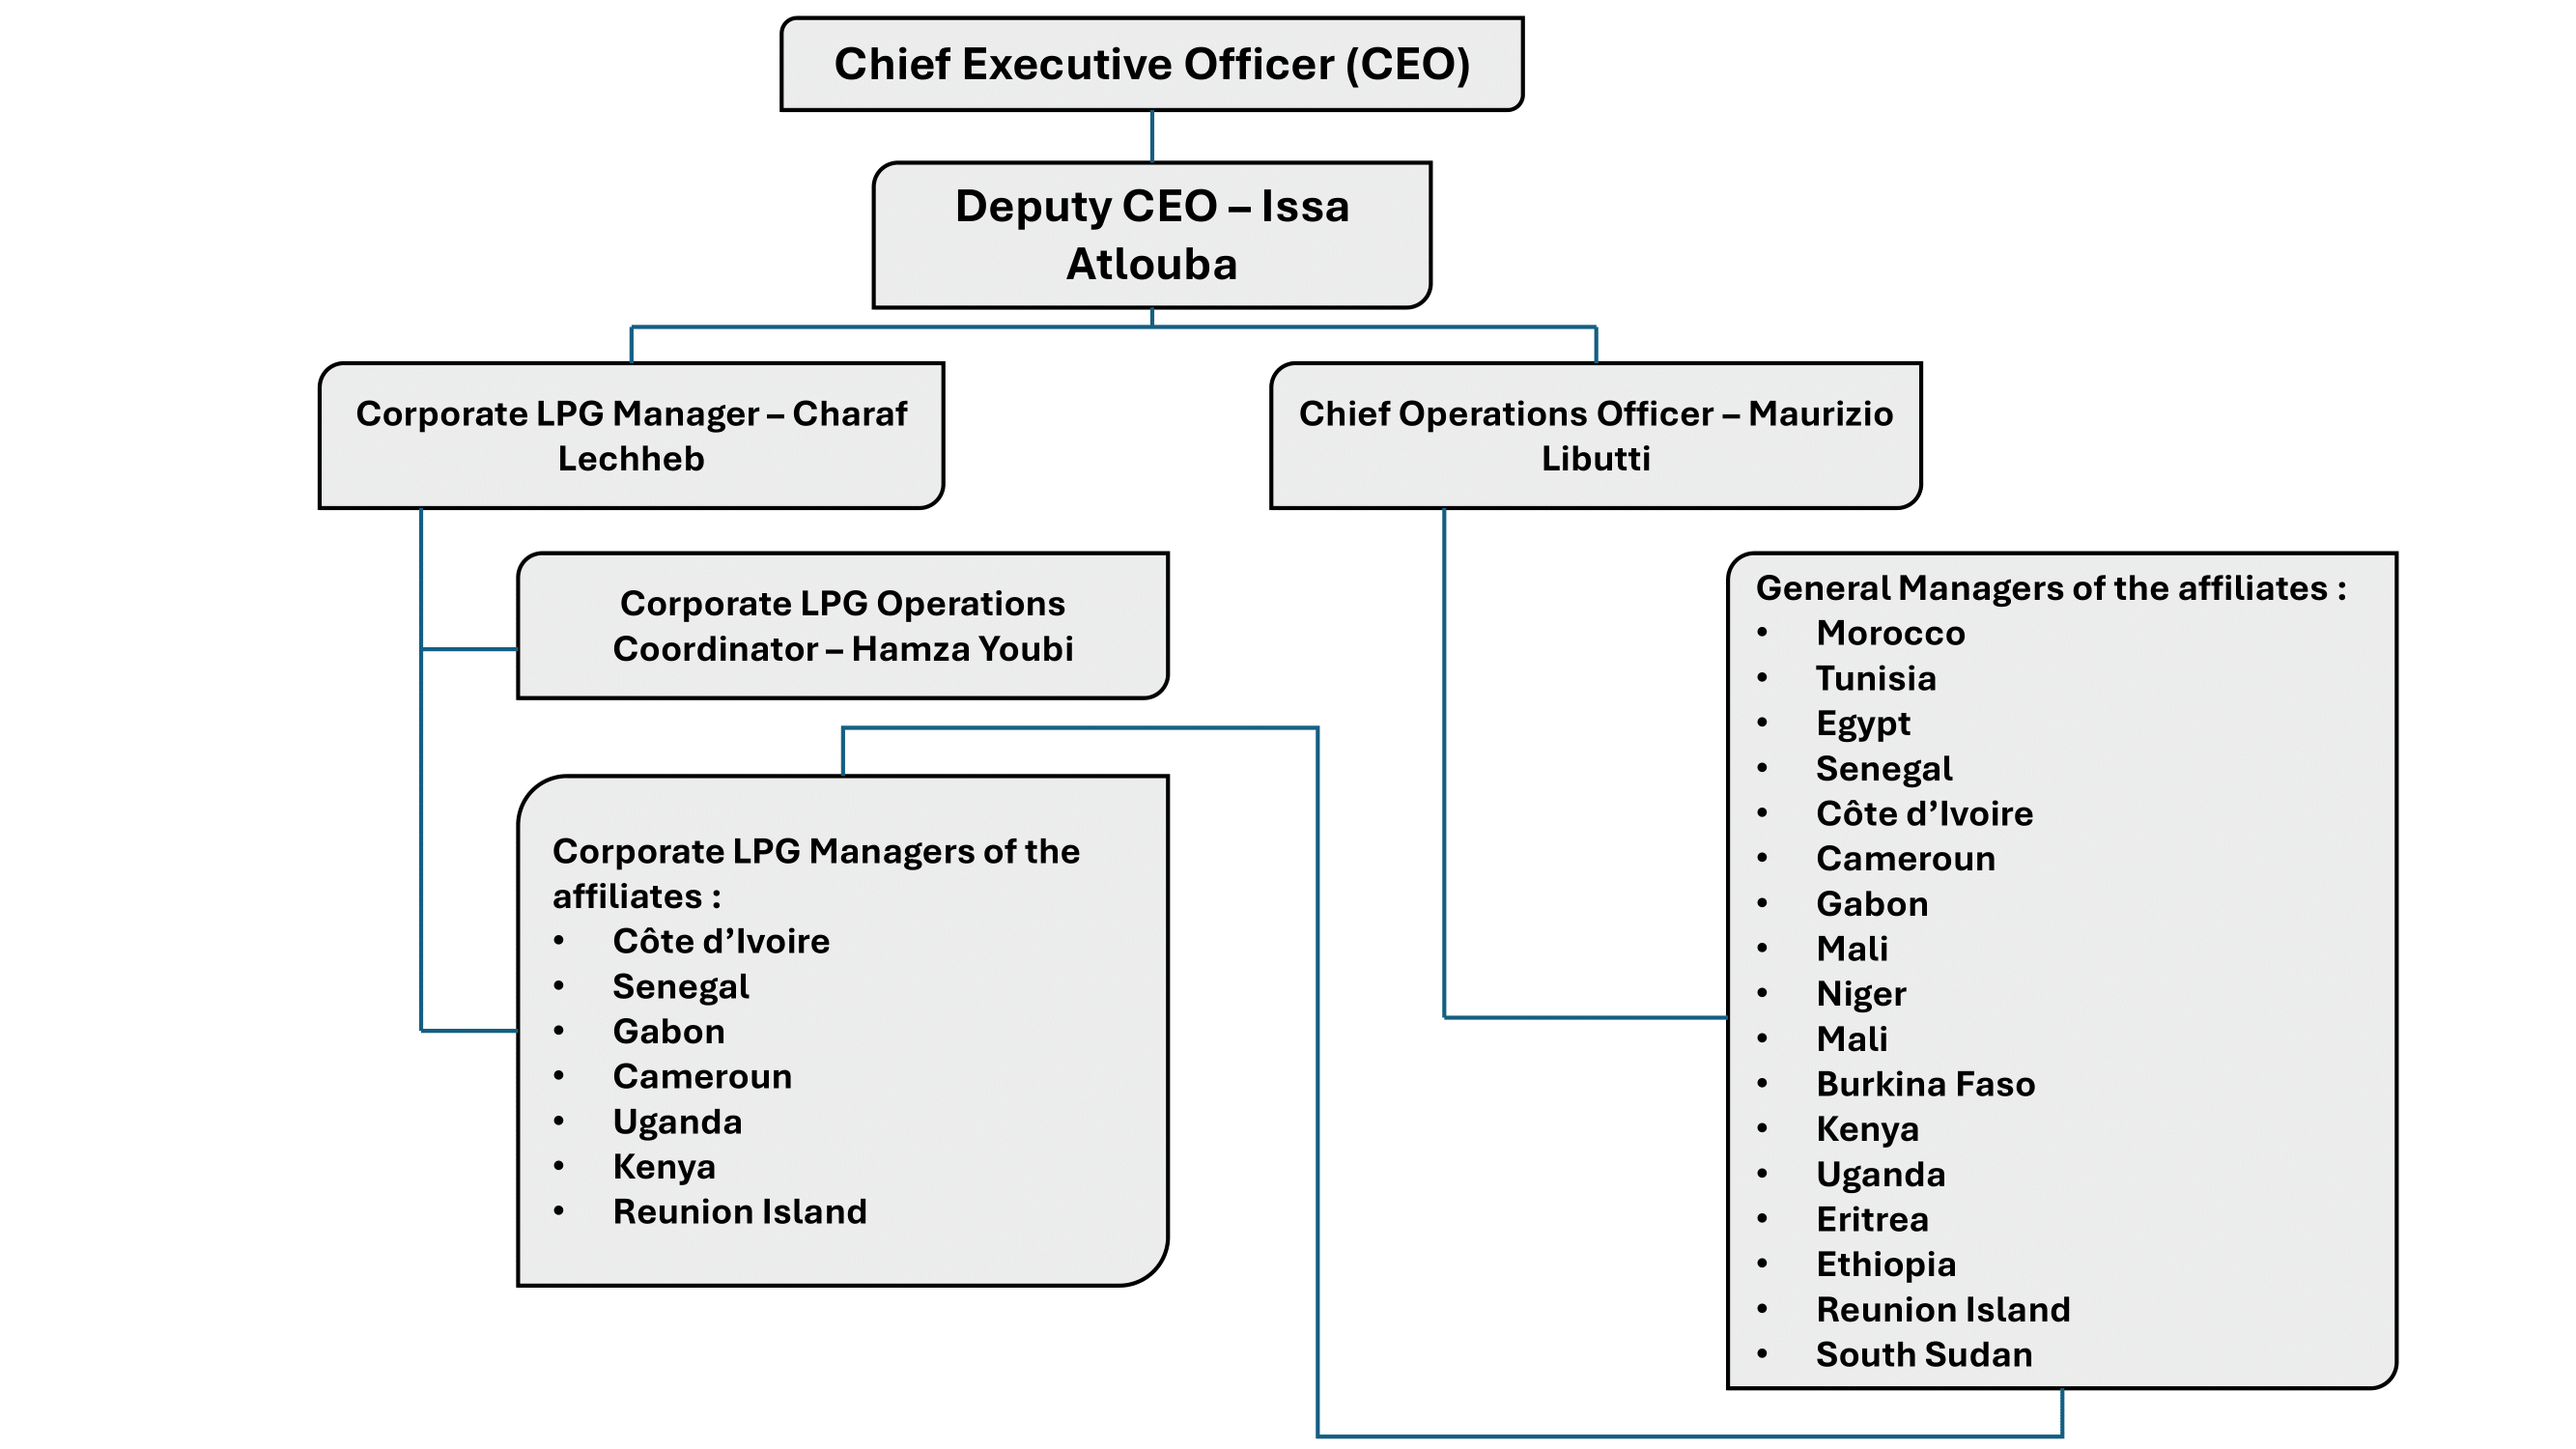
\includegraphics[width=0.7\textwidth]{Organigramme OLA Energy-1.png} % chemin de l'image
    \caption{Organigramme OLA Energy}
    \label{fig:Organigramme OLA Energy}
\end{figure}
\chapter{Analyse et définition des besoins}
\section{Détermination des fonctionnalités}
La création d'une plateforme pour la gestion des inventaires nécessite une approche structurée pour répondre aux besoins essentiels des utilisateurs. Le besoin primordial est le suivi précis des inventaires journaliers. Cette fonctionnalité doit permettre aux utilisateurs d'enregistrer les niveaux d'inventaire au début et à la fin de chaque journée d'activité. En offrant une vue claire des quantités disponibles, la plateforme permet de détecter rapidement les écarts et d'ajuster les stocks en conséquence. La saisie quotidienne des données garantit une traçabilité complète et une gestion proactive des stocks, ce qui est crucial pour maintenir l'exactitude des niveaux d'inventaire.
\\
\\
En complément de cette fonctionnalité, il est essentiel de mettre en place un système efficace pour le suivi des mouvements quotidiens des produits. Cette fonctionnalité doit permettre l'enregistrement détaillé de chaque entrée et sortie de stock. Suivre les mouvements en temps réel offre une vue complète des transactions journalières, ce qui aide à gérer les niveaux de stock de manière optimale. Une telle visibilité facilite également la planification et l'optimisation des processus logistiques, contribuant ainsi à une gestion plus fluide et réactive des inventaires.
\\
\\
Enfin, un tableau de réconciliation robuste est nécessaire pour compléter la gestion des inventaires. Ce tableau permet de comparer les données d'inventaire avec les mouvements enregistrés sur une période spécifiée, offrant ainsi un contrôle approfondi de la gestion des stocks. La réconciliation aide à identifier les incohérences, à vérifier l'exactitude des informations et à ajuster les enregistrements si nécessaire. En fournissant une analyse détaillée et un mécanisme de contrôle, le tableau de réconciliation assure la précision des données et contribue à une gestion rigoureuse des stocks.
\\
\\
En résumé, les besoins pour la plateforme incluent un suivi précis des inventaires journaliers, un enregistrement détaillé des mouvements quotidiens des produits, et un tableau de réconciliation pour le contrôle des stocks. Ces fonctionnalités sont essentielles pour garantir une gestion efficace des inventaires et une prise de décision éclairée.
\section{Étude du système déja existant}
L'analyse du fichier BASSA.xlsm, fourni par l'entreprise, révèle plusieurs lacunes significatives en termes de structure et d'efficacité du code. Ces observations mettent en évidence des domaines nécessitant des améliorations substantielles pour optimiser la gestion des données et garantir la pérennité du système.

\subsection{Structure du Code et Modularité :}
La structure actuelle du code dans BASSA.xlsm présente des défauts majeurs en matière de modularité, ce qui complique considérablement la maintenance et l'évolution du fichier. Le code n'est pas adéquatement réparti, rendant difficile l'isolation et la résolution des problèmes spécifiques. Une refonte vers une approche modulaire, avec des fonctions et des procédures distinctes, améliorerait notablement la lisibilité et la flexibilité du code. Cela faciliterait également les mises à jour et les modifications futures, minimisant les risques de perturbations dans le système global.
\begin{figure}[h]
    \centering
    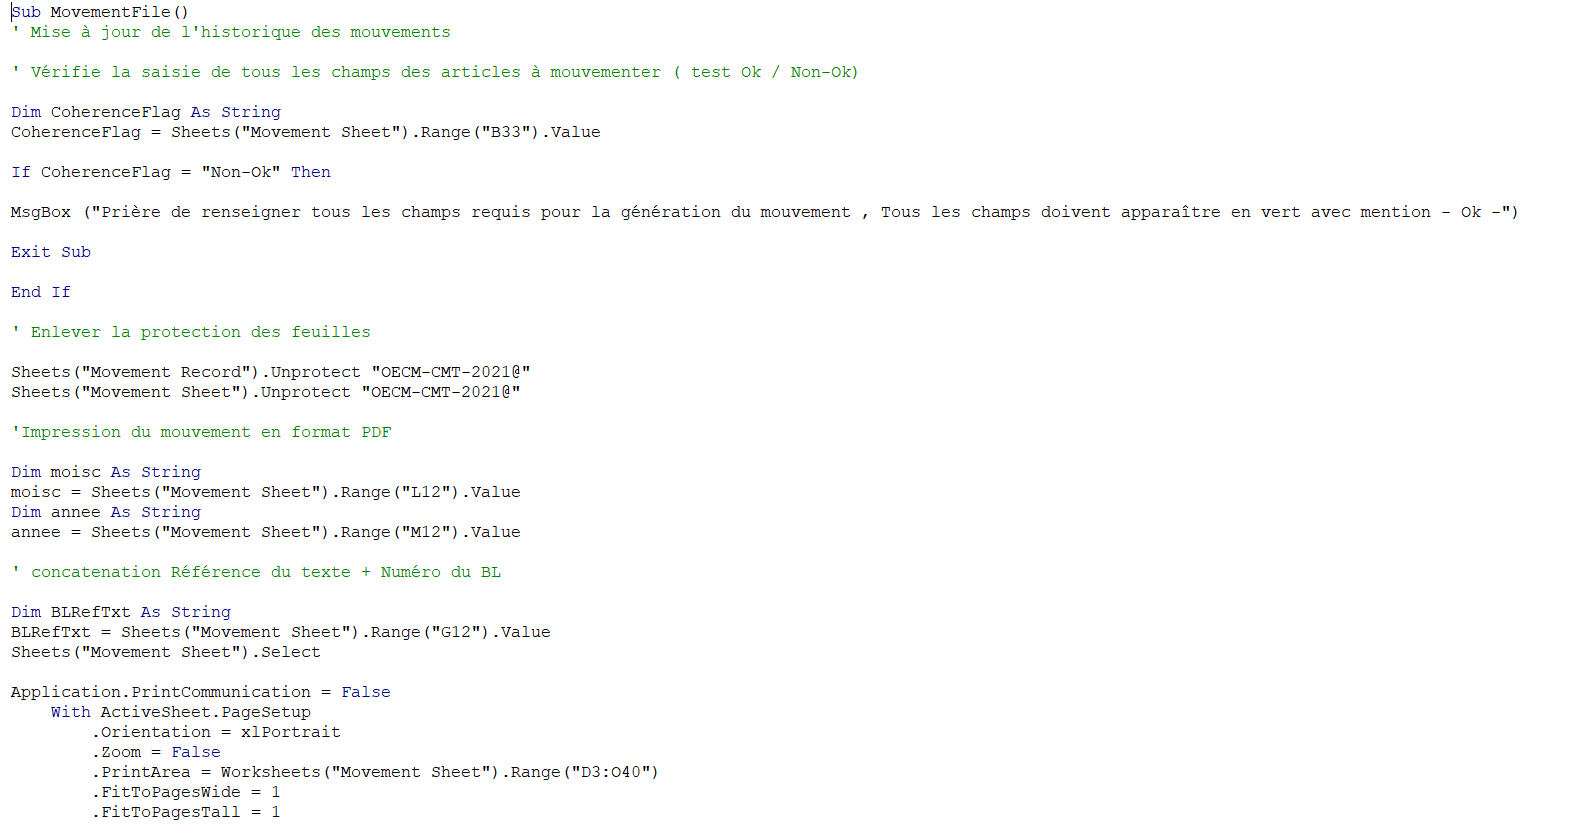
\includegraphics[width=0.9\textwidth]{Capture1.png} % chemin de l'image
    \caption{Problème de modularité}
    \label{fig:Problème de modularité}
\end{figure}

\subsection{Utilisation des Fonctions Prédéfinies :}
Le fichier s'appuie fortement sur les fonctions prédéfinies d'Excel, ce qui ne répond pas toujours aux besoins spécifiques de gestion des données de l'entreprise. Bien que ces fonctions soient adaptées pour des opérations générales, elles ne sont pas nécessairement conçues pour des exigences de traitement complexes ou personnalisées. Il est recommandé d'intégrer des fonctions personnalisées et adaptées aux besoins spécifiques de l'entreprise pour améliorer la précision et la flexibilité du traitement des données.
\begin{figure}[h]
    \centering
    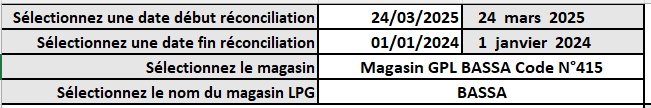
\includegraphics[width=0.7\textwidth]{Capture4.png} % chemin de l'image
    \caption{Exemple d'un problème logique}
    \label{Exemple d'un problème logique}
\end{figure}

\subsection{Gestion des Erreurs :}
La gestion des erreurs dans BASSA.xlsm est insuffisante, ce qui engendre des problèmes de cohérence dans la base de données. L'absence de mécanismes robustes pour la gestion des erreurs peut entraîner des entrées incorrectes ou incomplètes, compromettant ainsi l'intégrité des données. Il est impératif de mettre en œuvre des contrôles d'erreurs plus rigoureux et des validations systématiques pour assurer que les données sont correctement enregistrées et traitées.
\begin{figure}[h]
    \centering
    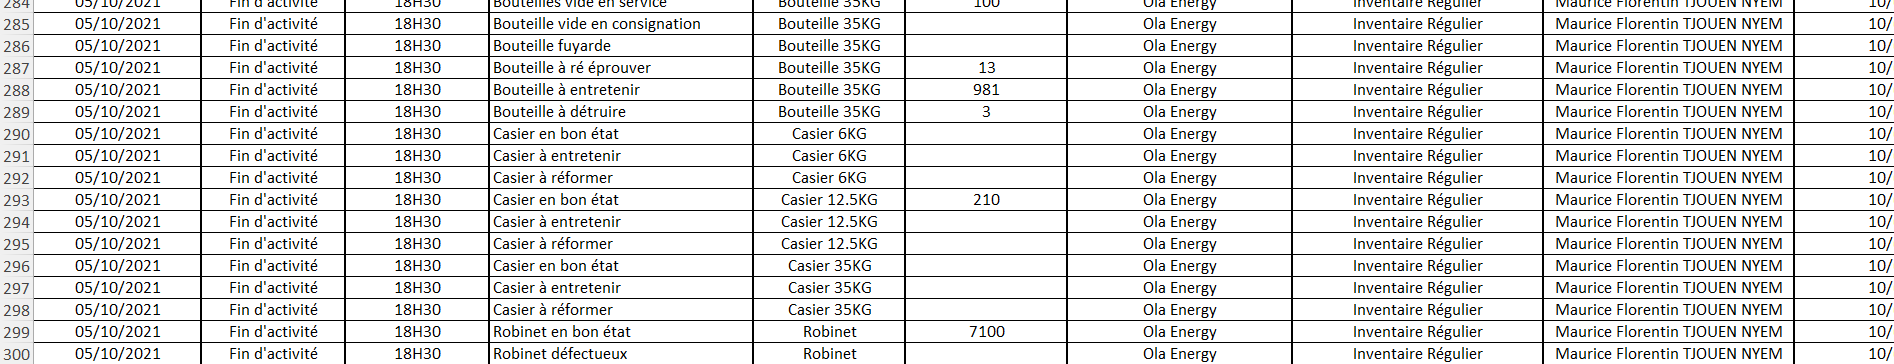
\includegraphics[width=0.9\textwidth]{Capture3.png} % chemin de l'image
    \caption{Problème d'incohérence de la base de donnés}
    \label{fig:Problème d'incohérence de la base de donnés}
\end{figure}

\subsection{Rigidité du Système :}
Le système en place démontre une rigidité qui le rend difficile à adapter aux évolutions futures. La structure actuelle semble peu flexible et ne permet pas d'ajustements ou de modifications aisés pour répondre aux nouvelles exigences. Il est nécessaire de concevoir un système plus adaptable, doté d'une architecture permettant des extensions et des modifications, afin de garantir sa pérennité et sa capacité à évoluer en fonction des besoins futurs.

\subsection{Type d'Interface :}
Actuellement, le fichier BASSA.xlsm présente une interface statique qui ne s'adapte pas aux sélections de l'utilisateur. Les menus et les options disponibles ne changent pas en fonction des choix effectués par l'utilisateur, ce qui limite la flexibilité et l'intuitivité de l'application. Une interface dynamique est essentielle pour améliorer l'expérience utilisateur en permettant aux choix et aux options d'être ajustés automatiquement en fonction des sélections faites. Cette fonctionnalité offrirait une interaction plus fluide et personnalisée, répondant mieux aux besoins spécifiques des utilisateurs.

\subsection{Sécurité :}
La sécurité du fichier est actuellement insuffisante, permettant à tout utilisateur d'accéder à la base de données. Il est crucial de renforcer la gestion des accès et de mettre en place des mécanismes de sécurité appropriés pour protéger les informations sensibles et éviter les manipulations non autorisées. La mise en œuvre de contrôles d'accès stricts est indispensable pour sécuriser les données et réduire les risques de compromission.

En conclusion, le fichier BASSA.xlsm présente plusieurs faiblesses notables en matière de structure du code, de modularité, de gestion des erreurs, de flexibilité et de sécurité. Il est fortement recommandé de procéder à une révision approfondie de ces aspects afin d'optimiser la fonctionnalité et la sécurité du système de gestion des inventaires
\begin{figure}[h]
    \centering
    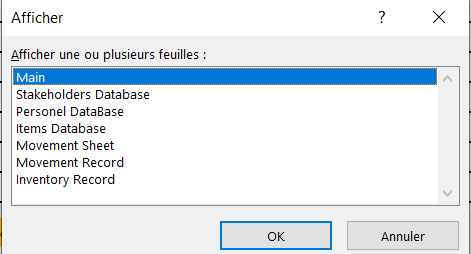
\includegraphics[width=0.7\textwidth]{Capture2.png} % chemin de l'image
    \caption{Problème de sécurité}
    \label{fig:Problème de sécurité}
\end{figure}
\section{Objectifs principales}
L’évaluation du fichier BASSA.xlsm a révélé plusieurs contraintes critiques qui nécessitent une attention particulière pour aligner le système avec les besoins de l’entreprise. Les objectifs principaux doivent être révisés en fonction de ces contraintes afin d’optimiser la gestion des données et d’améliorer l’efficacité globale du système.

\subsection{Amélioration de la Modularité et de la Maintenance du Code}
\textsc{Contraintes} : La structure du code est actuellement peu modulaire, rendant difficile la maintenance et l'évolution du fichier.

\textsc{Analyse} : Pour atteindre cet objectif, il est impératif de refondre le code en modules clairement définis, chacun ayant une responsabilité spécifique. Une approche modulaire permet de séparer les préoccupations et facilite la gestion du code en isolant les fonctionnalités distinctes. Cela améliore la lisibilité, simplifie la maintenance et permet des modifications ciblées sans affecter l’ensemble du système. En outre, cette modularité facilite les tests unitaires et le débogage, assurant ainsi une meilleure qualité du code et une plus grande résilience face aux évolutions futures.

\subsection{Optimisation de la Flexibilité des Fonctions}
\textsc{Contraintes} : Le système utilise des fonctions prédéfinies d'Excel qui ne répondent pas toujours aux besoins spécifiques de l'entreprise.

\textsc{Analyse} : Pour répondre à cet objectif, il est nécessaire de développer des fonctions personnalisées adaptées aux exigences spécifiques de gestion des données de BASSA. Les fonctions prédéfinies d'Excel, bien que puissantes, peuvent être limitées dans des scénarios complexes. La création de fonctions sur mesure permettra de traiter des cas particuliers, d’optimiser les performances et d’améliorer la précision des opérations. Par exemple, des fonctions personnalisées peuvent intégrer des logiques métier spécifiques, gérer des formats de données particuliers ou automatiser des tâches complexes non couvertes par les fonctions standard.

\subsection{Renforcement de la Gestion des Erreurs et de la Cohérence des Données}
\textsc{Contraintes} : La gestion des erreurs est insuffisante, entraînant des incohérences dans la base de données.

\textsc{Analyse} : L’amélioration de la gestion des erreurs doit inclure la mise en œuvre de contrôles et de validations systématiques tout au long du processus de traitement des données. L’objectif est d’introduire des mécanismes de capture des erreurs, des alertes en cas de données incorrectes, et des routines de correction automatique lorsque cela est possible. Cette approche proactive assurera la cohérence des données en détectant et en rectifiant les erreurs avant qu’elles n’affectent l’intégrité globale du système. Par exemple, des validations de saisie, des vérifications de cohérence et des contrôles de qualité doivent être intégrés pour garantir que les données saisies sont correctes et conformes aux exigences.

\subsection{Amélioration de la Flexibilité et de l’Adaptabilité du Système}
\textsc{Contraintes} : Le système actuel est rigide et difficile à adapter aux évolutions futures.

\textsc{Analyse} : Pour atteindre cet objectif, il est crucial de concevoir une architecture système flexible qui permet des ajustements aisés et des extensions futures. La mise en place d’une architecture évolutive, avec des interfaces modulables et des mécanismes d'intégration ouverts, facilitera l’adaptation aux nouvelles exigences et technologies. Cela pourrait inclure la mise en place de couches d’abstraction, l’utilisation de services web ou d’API pour l’intégration, et la conception de structures de données extensibles. Une telle flexibilité garantit que le système peut évoluer avec les besoins de l’entreprise sans nécessiter de refontes majeures.

\subsection{Renforcement de la Sécurité des Données}
\textsc{Contraintes} : La sécurité du fichier est insuffisante, permettant un accès non autorisé à la base de données.

\textsc{Analyse} : Le renforcement de la sécurité des données implique la mise en œuvre de contrôles d’accès stricts, d’authentifications robustes, et de mécanismes de cryptage des données sensibles. L’objectif est d’assurer que seules les personnes autorisées peuvent accéder et manipuler les données. Cela nécessite la configuration de rôles et de permissions pour contrôler l’accès aux différentes sections du système et l’utilisation de protocoles de sécurité pour protéger les informations contre les intrusions. De plus, la mise en place de journaux d’audit et de systèmes de surveillance renforcera la capacité à détecter et à répondre aux tentatives d'accès non autorisées.

\subsection{Création d’une Interface Dynamique et Intuitive}
\textsc{Contraintes} : L’interface actuelle est statique et ne s’adapte pas aux choix de l’utilisateur.

\textsc{Analyse} : Pour répondre à cet objectif, il est nécessaire de concevoir une interface utilisateur dynamique qui adapte les options et les informations en fonction des actions et des sélections de l’utilisateur. Une interface dynamique améliore l’expérience utilisateur en rendant le système plus interactif et réactif aux besoins individuels. Cela pourrait inclure des éléments tels que des menus contextuels interactifs, des filtres dynamiques et des champs de saisie qui se mettent à jour en fonction des choix précédents. Cette adaptabilité offre une navigation plus fluide et personnalisée, réduisant ainsi le risque de confusion et d’erreurs, et augmentant l’efficacité de l’utilisation du système.

En conclusion, les objectifs principaux de BASSA doivent être réévalués et améliorés en fonction des contraintes identifiées pour optimiser la fonctionnalité, la sécurité et l’efficacité du système de gestion des inventaires. En adressant ces objectifs de manière approfondie, BASSA pourra développer un système plus robuste, flexible et sécurisé, répondant mieux aux besoins actuels et futurs de l’entreprise.
\section{Définition des besoins}
\subsection{Gestion des utilisateurs}
La définition claire des rôles des utilisateurs est cruciale pour assurer un fonctionnement optimal, sécurisé et efficace du système de gestion des inventaires. Chaque utilisateur se voit attribuer des permissions spécifiques en fonction de ses responsabilités et de ses besoins opérationnels.

\subsubsection{Administrateur}

L'administrateur est le gestionnaire suprême du système. Il possède tous les droits nécessaires pour effectuer des opérations de gestion complète sur l'application. Son rôle est central et implique plusieurs responsabilités, notamment :

\begin{itemize}
    \item \textbf{Gestion des utilisateurs} : L'administrateur peut créer, modifier ou supprimer les comptes des autres utilisateurs (manager, magasinier, sales, reconciliation). Il attribue des rôles, met à jour les informations d'accès et ajuste les permissions.
    \item \textbf{Paramétrage du système} : Il est responsable de la configuration et de la personnalisation de l'application selon les besoins de l'organisation, incluant la gestion des accès, des vues, et des fonctions disponibles pour chaque type d'utilisateur.
    \item \textbf{Surveillance et audit} : L'administrateur est en mesure de visualiser les journaux d'audit et d'activité, d'assurer la conformité avec les politiques internes et de détecter toute anomalie ou activité suspecte.
\end{itemize}

L'administrateur est ainsi le garant du bon fonctionnement de l'application et de la sécurité des données, agissant comme un superviseur de haut niveau.

\subsubsection{Manager}

Le rôle du manager se concentre principalement sur la gestion des opérations au sein de l'application. Contrairement à l'administrateur, ses permissions sont limitées pour des raisons de sécurité et de division des responsabilités :

\begin{itemize}
    \item \textbf{Visualisation et consultation des données} : Le manager peut accéder à toutes les données relatives aux produits, aux mouvements de stock et aux inventaires, lui permettant de suivre en temps réel l'état des stocks.
    \item \textbf{Rapports et analyses} : Il a la capacité de générer des rapports et d'effectuer des analyses sur les données disponibles pour la prise de décision stratégique.
    \item \textbf{Coordination des équipes} : Il peut superviser les opérations des autres utilisateurs (magasinier, sales, reconciliation) sans avoir la capacité de manipuler leurs droits ou leurs accès.
\end{itemize}

Le manager est donc un acteur clé pour le suivi de l'activité et la prise de décisions, sans pour autant pouvoir altérer les configurations du système.

\subsubsection{Magasinier}

Le magasinier est le seul utilisateur autorisé à entrer des données dans l'application. Ce rôle est spécialisé et se concentre sur la saisie et la mise à jour des informations liées aux mouvements de stock :

\begin{itemize}
    \item \textbf{Entrée de données} : Il peut ajouter, modifier ou supprimer des données relatives aux produits, aux stocks entrants et sortants, et aux inventaires quotidiens.
    \item \textbf{Gestion des stocks} : En tant que responsable des données d'entrée, le magasinier assure que les enregistrements sont corrects, à jour et en accord avec la réalité du terrain.
\end{itemize}

Ce rôle est essentiel pour la fiabilité des données présentes dans l'application, étant donné que le magasinier est le seul utilisateur habilité à manipuler ces données.

\subsubsection{Sales}

Le rôle de l'utilisateur "Sales" se limite à la consultation des données de la base de données sans aucune capacité de modification. Ce rôle est destiné aux utilisateurs qui ont besoin d'accéder aux informations de l'inventaire pour des analyses, des rapports ou des présentations, sans interférer avec les opérations :

\begin{itemize}
    \item \textbf{Visualisation des données} : L'utilisateur Sales peut consulter toutes les informations de la base de données mais ne peut pas ajouter, modifier ou supprimer les données.
    \item \textbf{Rapports et suivis} : Bien qu'il ne puisse pas modifier les données, il peut visualiser des rapports générés et effectuer des suivis sur les ventes et les mouvements de stock.
\end{itemize}

Le rôle Sales assure ainsi une consultation sécurisée des données pour le personnel concerné, sans risques de manipulation accidentelle ou malveillante.

\subsubsection{Réconciliation}

L'utilisateur "Reconciliation" joue un rôle spécifique dans le processus de contrôle 
\begin{itemize}
    \item \textbf{Manipulation du tableau de réconciliation} : Cet utilisateur est autorisé à manipuler le tableau de réconciliation, permettant ainsi de vérifier la cohérence des mouvements de stock et de s'assurer que toutes les transactions sont correctement enregistrées.
    \item \textbf{Visualisation des données} : Comme l'utilisateur Sales, l'utilisateur Reconciliation peut également consulter toutes les données de la base de données sans la capacité de les modifier.
    \item \textbf{Contrôle des stocks} : Il a un rôle important dans le contrôle de la gestion des stocks et peut signaler toute anomalie ou erreur de données.
\end{itemize}

L'utilisateur Reconciliation apporte une couche supplémentaire de contrôle et d'assurance qualité, en veillant à ce que les informations stockées soient exactes et conformes aux mouvements physiques des stocks.



La distinction entre les rôles d'administrateur, manager, magasinier, sales, et reconciliation est essentielle pour maintenir une organisation claire et sécurisée dans l'application de gestion des inventaires. Chaque rôle a des responsabilités spécifiques et des permissions limitées en fonction des besoins opérationnels. Cela permet non seulement d'assurer la sécurité des données et l'intégrité du système, mais aussi de faciliter une utilisation efficace et ciblée de l'application par les différents intervenants. Une telle séparation des tâches est cruciale pour une gestion rigoureuse et efficace des inventaires au sein de toute organisation.

\subsection{Éviter les DEADLOCKS}
\subsubsection{Introduction}
Dans le contexte d'une application de gestion des inventaires, la saisie et la mise à jour des données de stock sont des opérations critiques qui doivent être exécutées de manière fluide et sécurisée. Les transactions impliquant la manipulation des données de stock, telles que l'ajout, la modification ou la suppression des enregistrements, doivent être réalisées de manière à éviter les interblocages (deadlocks) qui peuvent paralyser le système et nuire à la continuité des opérations. Ainsi, il est essentiel de définir des stratégies et des mécanismes efficaces pour prévenir ces situations de blocage et garantir une gestion optimisée des transactions.

\subsubsection{Définition du Deadlock}
Un deadlock ou interblocage est une situation dans laquelle deux ou plusieurs transactions ou processus se bloquent mutuellement en attendant que l'autre libère une ressource. Dans le contexte d'une application de gestion des stocks, cela peut se produire lorsque plusieurs utilisateurs ou processus tentent simultanément d'accéder aux mêmes enregistrements de données, en essayant de les verrouiller pour modification ou mise à jour. Par exemple, si le Magasinier A tente de mettre à jour l'état de stock d'un produit pendant que le Magasinier B essaye de supprimer ce même produit de l'inventaire, un deadlock peut survenir si chaque transaction attend que l'autre libère le verrou.

\subsubsection{Importance de la Prévention des Deadlocks}
La prévention des deadlocks est essentielle pour plusieurs raisons :
\begin{itemize}


\item \textbf{Continuité des Opérations :} Les deadlocks peuvent entraîner des blocages dans les processus de saisie et de mise à jour des données, perturbant ainsi la continuité des opérations de gestion des stocks. Éviter ces blocages permet de maintenir un flux constant de transactions et d'opérations critiques, réduisant ainsi le temps d'attente des utilisateurs et les interruptions.

\item \textbf{Amélioration des Performances du Système :} Lorsque des deadlocks se produisent, les ressources du système sont consommées inutilement par des transactions en attente. Cela peut entraîner une diminution des performances globales de l'application et affecter négativement l'expérience utilisateur. En prévenant les deadlocks, on optimise l'utilisation des ressources et on garantit une réactivité accrue du système.

\item \textbf{Sécurité et Intégrité des Données :} Les deadlocks peuvent également compromettre l'intégrité des données. Lorsque des transactions sont bloquées ou annulées en raison d'interblocages, il y a un risque que certaines modifications ne soient pas correctement enregistrées ou que les données deviennent incohérentes. La prévention des deadlocks contribue donc à la sécurité des données en assurant leur exactitude et leur fiabilité.

\item \textbf{Réduction des Risques de Pertes Financières et Opérationnelles :} Dans un environnement de gestion d'inventaire, où les décisions sont souvent prises en temps réel en fonction des données disponibles, les deadlocks peuvent retarder des décisions critiques et entraîner des pertes financières et opérationnelles. En éliminant ces blocages, on réduit les risques de pertes et on assure une gestion efficace des stocks.
\end{itemize}
\subsubsection{Stratégies de Prévention des Deadlocks}
Pour répondre à ce besoin crucial, plusieurs stratégies peuvent être mises en œuvre afin d'éviter les deadlocks dans la gestion des transactions de saisie de données :
\begin{itemize}
\item \textbf{Ordonnancement des Transactions :} Imposer un ordre strict pour l'accès aux ressources peut aider à éviter les deadlocks. Par exemple, les transactions peuvent être conçues de manière à toujours accéder aux ressources dans un ordre prédéfini. Cela réduit les chances que deux transactions se verrouillent mutuellement en attendant des ressources.

\item \textbf{Utilisation de Verrouillages Temporels (Timeouts) :} Configurer des mécanismes de temporisation pour les verrous peut empêcher les transactions de rester bloquées indéfiniment. Si une transaction ne parvient pas à acquérir un verrou après un certain délai, elle est annulée ou mise en attente pour être réessayée plus tard, évitant ainsi un interblocage potentiel.

\item \textbf{Transactions Atomiques et Granulaires :} Diviser les transactions complexes en opérations plus petites et atomiques peut minimiser les risques de deadlocks. Les petites transactions sont moins susceptibles de se bloquer entre elles et peuvent être traitées plus rapidement.

\item \textbf{Détection et Reprise après Deadlock :} Mettre en place un mécanisme de détection de deadlock et une stratégie de reprise permet de surveiller activement les transactions et de prendre des mesures correctives lorsque des deadlocks sont détectés. Cela peut inclure l'annulation de certaines transactions pour libérer des ressources.

\item \textbf{Verrouillage Optimiste :} Au lieu d'utiliser un verrouillage pessimiste (qui bloque les ressources dès le début de la transaction), le verrouillage optimiste permet aux transactions de lire les données sans verrouillage, en vérifiant ensuite si des conflits se sont produits avant de finaliser l'opération. Cela réduit la probabilité de deadlocks.
\end{itemize}
\subsubsection{Conclusion}
La prévention des deadlocks dans la gestion des transactions de saisie de données est un besoin fondamental pour garantir le bon fonctionnement et la performance d'une application de gestion des stocks. En mettant en œuvre des stratégies efficaces pour éviter ces blocages, on améliore la continuité des opérations, l'intégrité des données, les performances du système, et on réduit les risques de pertes financières. La gestion proactive des deadlocks est donc essentielle pour toute organisation cherchant à optimiser ses processus de gestion des stocks et à garantir la fiabilité et la sécurité de son système d'information.
\subsection{Développement d'une application mobile}
\subsubsection{Introduction}
Dans un monde de plus en plus connecté et mobile, les entreprises cherchent à améliorer leur efficacité opérationnelle et à optimiser leurs processus en offrant plus de flexibilité à leurs utilisateurs. Un des besoins majeurs de notre entreprise est de développer une application mobile intégrée capable de réaliser tous les traitements nécessaires liés à la gestion des inventaires, des stocks, des ventes, et des autres opérations. Cette application mobile viendra compléter le système existant sur PC, offrant ainsi une solution hybride qui sera plus bénéfique et plus adaptée aux réalités des opérations modernes.

\subsubsection{Limites d'un Système Uniquement sur PC}
Actuellement, la majorité des opérations de gestion sont effectuées via une application ou un système installé sur des ordinateurs de bureau ou des PC portables. Bien que cette approche ait été efficace dans le passé, elle présente plusieurs limitations dans le contexte actuel de la digitalisation et de la mobilité accrue :
\begin{itemize}


\item \textbf{Manque de Flexibilité et de Mobilité :} Les utilisateurs sont limités à effectuer leurs tâches à partir de leur poste de travail fixe. Cela n'est pas optimal pour les utilisateurs sur le terrain, comme les magasiniers, les agents de vente, ou les responsables de contrôle d'inventaire, qui doivent souvent se déplacer dans l'entrepôt, le magasin ou d'autres installations.

\item \textbf{Accès Limité en Temps Réel :} L'absence de mobilité réduit la capacité à accéder aux informations en temps réel, ce qui est crucial pour la prise de décision rapide et la gestion efficace des stocks et des ventes.

\item \textbf{Adaptabilité Restreinte aux Nouveaux Modèles de Travail :} Avec l'augmentation du télétravail, des déplacements fréquents et des besoins de travail collaboratif, les systèmes exclusivement sur PC deviennent de moins en moins adaptés aux besoins modernes d'adaptabilité et de connectivité.
\end{itemize}
\subsubsection{Avantages d'une Application Mobile Complète}
La création d'une application mobile complète, qui gère tous les traitements possibles, présente plusieurs avantages par rapport à un système seulement basé sur PC. Voici les principales raisons pour lesquelles cette approche serait plus bénéfique :
\begin{itemize}
\item \textbf{Mobilité et Flexibilité Accrues :} Une application mobile permet aux utilisateurs d'accéder au système à tout moment et en tout lieu, offrant ainsi une flexibilité incomparable. Que ce soit pour la saisie des données, le suivi des stocks, la gestion des ventes ou la réconciliation des inventaires, les utilisateurs peuvent effectuer leurs tâches sur le terrain, en déplacement ou à distance, sans être liés à un poste fixe.

\item \textbf{Mise à Jour des Données en Temps Réel :} Grâce à la connectivité mobile et à la synchronisation via le cloud, les utilisateurs peuvent mettre à jour les informations en temps réel. Cela garantit que toutes les données sont toujours à jour, ce qui est essentiel pour la gestion efficace des stocks, l'optimisation des ventes et la prise de décision rapide.

\item \textbf{Amélioration de l'Efficacité Opérationnelle :} Une application mobile intégrée réduit les temps d'attente et les étapes intermédiaires. Par exemple, un magasinier peut immédiatement scanner des produits, enregistrer les mouvements de stock, et mettre à jour le système sans avoir à retourner à un bureau, ce qui augmente considérablement l'efficacité opérationnelle.

\item \textbf{Meilleure Expérience Utilisateur :} Les applications mobiles modernes peuvent offrir une interface utilisateur intuitive, simplifiée et adaptée aux petits écrans, ce qui rend la navigation et l'exécution des tâches plus faciles et plus rapides par rapport aux systèmes PC traditionnels.

\item \textbf{Intégration de Fonctionnalités Spécifiques au Mobile :} Les applications mobiles peuvent tirer parti de fonctionnalités spécifiques telles que la géolocalisation, les notifications push, la reconnaissance vocale, les caméras pour la lecture de codes-barres ou QR codes, et bien d'autres, qui peuvent améliorer les processus de gestion des stocks et des ventes.
\end{itemize}
\subsubsection{Communication Centralisée via le Cloud et une Base de Données Unique}
Pour maximiser l'efficacité et garantir une cohérence parfaite entre les différents systèmes (PC et mobile), il est crucial que les deux applications (mobile et PC) communiquent via un cloud centralisé et partagent une base de données unique. Cette approche offre de nombreux avantages supplémentaires :
\begin{itemize}
\item \textbf{Synchronisation des Données en Temps Réel :} En centralisant la base de données dans le cloud, toutes les données saisies via l'application mobile ou le système PC sont instantanément synchronisées. Cela assure une mise à jour instantanée des informations sur tous les dispositifs, éliminant les incohérences et les doublons de données.

\item \textbf{Accessibilité Globale et Sécurisée :} Un système basé sur le cloud permet aux utilisateurs d'accéder de manière sécurisée aux données et aux fonctionnalités de l'application depuis n'importe où dans le monde, tant qu'ils ont une connexion Internet. Cela est essentiel pour les équipes de vente et les gestionnaires d'inventaire qui opèrent dans différentes régions.

\item \textbf{Maintenance et Mise à Jour Simplifiées :} En centralisant le système dans le cloud, les mises à jour et la maintenance du logiciel peuvent être effectuées de manière centralisée, ce qui réduit le besoin d'interventions sur chaque appareil individuel, que ce soit un PC ou un smartphone.

\item \textbf{Évolutivité et Adaptabilité :} Une architecture basée sur le cloud offre une grande évolutivité, permettant d'ajuster les ressources et les capacités en fonction de la croissance de l'entreprise et des besoins changeants.

\item \textbf{Sécurité Renforcée des Données :} Les solutions cloud modernes offrent des niveaux de sécurité élevés, y compris le cryptage des données, les contrôles d'accès granulaires, et les mécanismes de sauvegarde automatique, garantissant que les données de l'entreprise sont protégées contre les pertes ou les accès non autorisés.
\end{itemize}
\subsubsection{Conclusion}
Le besoin de développer une application mobile complète qui communique avec le système existant sur PC via un cloud centralisé et une base de données unique est un pas stratégique vers la modernisation des opérations de l'entreprise. Cette solution hybride offre non seulement une flexibilité et une mobilité accrues, mais elle améliore également l'efficacité, la sécurité, et la précision des processus de gestion. En investissant dans cette approche intégrée, l'entreprise pourra répondre plus efficacement aux besoins changeants de ses utilisateurs, tout en restant compétitive dans un environnement de plus en plus axé sur la mobilité et la connectivité.

\chapter{Analyse Fonctionelle}
\section{Diagramme de cas d'utlisation}

\subsection{Définition}
En langage de modélisation unifié (UML), un diagramme de cas d'utilisation peut 
servir à résumer les informations des acteurs et leurs actions avec votre système. La 
création de ce type de diagramme UML utilise un ensemble de symboles et de 
connecteurs spécifiques. Lorsqu'ils sont bien conçus, les diagrammes de cas 
d'utilisation peuvent aider à représenter : 
\begin{itemize}
\item Les scénarios dans lesquels votre système interagit avec des personnes, des 
organisations ou des systèmes externes ; 
\item Les objectifs que votre système ou application permet aux entités (appelées acteurs) 
d'atteindre ; 
\item La portée de votre système. 
\end{itemize}
Le diagramme de cas d’utilisation utilise trois relations importantes entre les actions 
qui sont :  
\begin{itemize}
\item \textbf{ Generalize :} qui signifie brièvement l’héritage entre les actions 
\item \textbf{ Include :} qui signifie la dépendance d’une action à l’autre (il faut qu’une action soit 
exécuté pour que l’autre soit aussi) 
\item \textbf{Extends :} qui fait référence à un cas spécial pour les actions dérivées du cas normale.  
\end{itemize}
\subsection{Réalisation}
\begin{figure}[h]
    \centering
    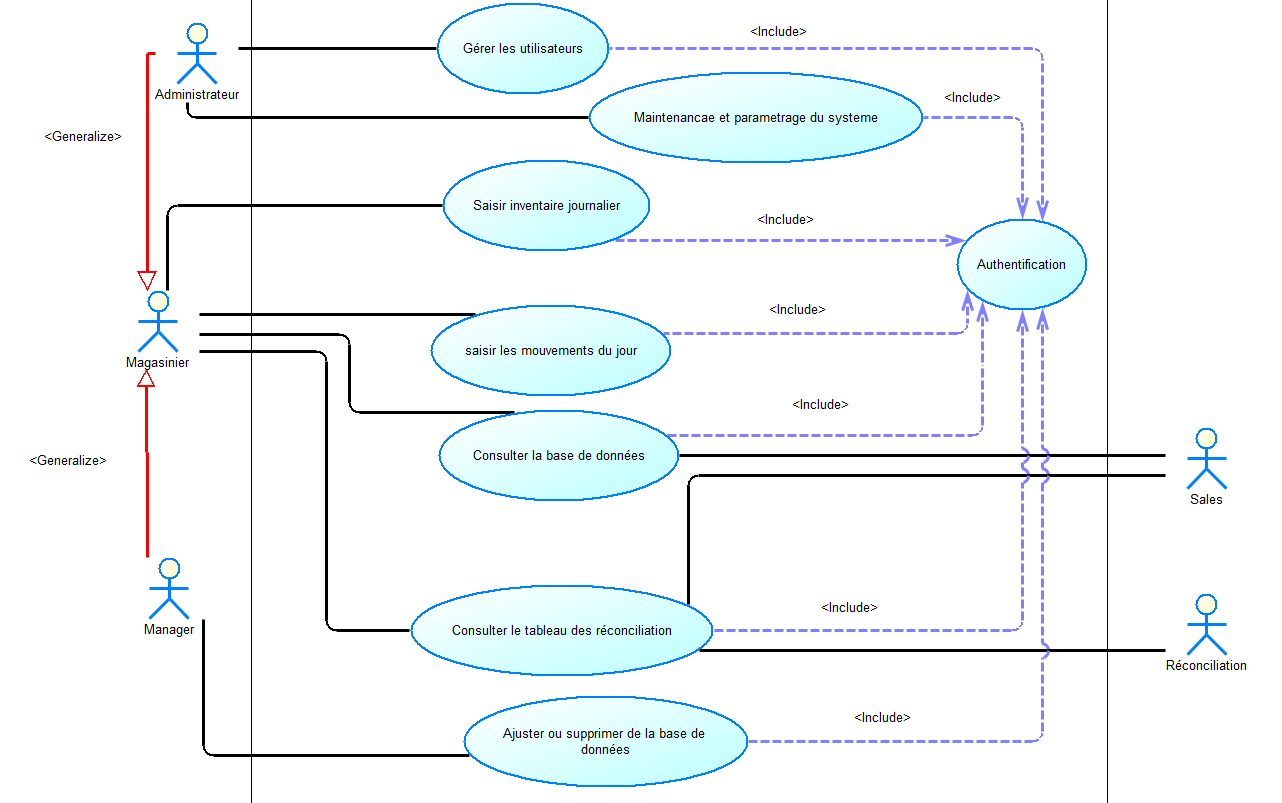
\includegraphics[width=1\textwidth]{USE CASE.png} % chemin de l'image
    \caption{Diagramme de cas d'utilisation}
    \label{fig:Diagramme de cas d'utilisation}
\end{figure}
\newpage
\subsection{Analsye}
\subsubsection{Introduction :}
Ce diagramme de cas d'utilisation représente les fonctionnalités principales du système, ainsi que les interactions entre les différents types d'utilisateurs et ces fonctionnalités. Les acteurs principaux identifiés sont l'Administrateur, le Magasinier, le Manager, le service des Ventes (Sales), et le service de Réconciliation.

\subsubsection{Acteurs :}
\begin{itemize}
\item \textbf{Administrateur :} Responsable de la gestion des utilisateurs et de la maintenance du système. Il dispose des droits les plus élevés et peut effectuer diverses actions critiques comme la gestion des utilisateurs et la maintenance du système.

\item \textbf{Magasinier :} Un utilisateur du système qui a des responsabilités liées à la saisie des inventaires et des mouvements quotidiens. Ce rôle est généralisé sous celui de l'Administrateur, ce qui suggère que le Magasinier pourrait hériter de certaines fonctionnalités de l'Administrateur.
\item \textbf{Manager :} Il est aussi généralisé sous le Magasinier, ce qui signifie qu'il peut effectuer les tâches d'un Magasinier en plus de ses propres tâches spécifiques.
\item \textbf{Sales (Ventes) :} Cet acteur interagit avec le système principalement pour consulter la base de données, probablement pour obtenir des informations pertinentes aux ventes.
\item \textbf{Réconciliation :} Cet acteur est en charge des activités de réconciliation, c’est-à-dire vérifier et ajuster les enregistrements pour s'assurer de leur exactitude.
\end{itemize}
\subsubsection{Cas d'Utilisation :}
Gérer les utilisateurs : Action principalement effectuée par l'Administrateur pour créer, modifier ou supprimer des comptes utilisateurs dans le système.
\begin{itemize}
\item \textbf{Maintenance et paramétrage du système :} Inclus dans plusieurs autres cas d'utilisation, cette fonctionnalité permet de maintenir le bon fonctionnement du système et de configurer ses paramètres pour répondre aux besoins des utilisateurs.
\item \textbf{Saisir l'inventaire journalier :} Un cas d'utilisation clé pour les Magasiniers, qui consiste à enregistrer les stocks journaliers dans le système.
\item \textbf{Saisir les mouvements du jour :} Impliquant la saisie des transactions quotidiennes, comme les entrées et sorties de stock.
\item \textbf{Consulter la base de données : }Permet aux utilisateurs de rechercher et d'afficher des informations stockées dans la base de données, crucial pour le service des Ventes et pour d'autres utilisateurs cherchant à vérifier des données.
\item \textbf{Consulter le tableau de réconciliation :} Une fonctionnalité spécifique pour vérifier les enregistrements, notamment en identifiant et en corrigeant les écarts dans les données.
\item \textbf{Ajuster ou supprimer de la base de données :} Permet de modifier ou de supprimer des données existantes, une fonctionnalité critique pour la gestion des stocks et la précision des enregistrements.
\end{itemize}
\subsubsection{Relation entre les Cas d'Utilisation :}
Le diagramme utilise les relations d'inclusion (« include ») pour indiquer que certaines fonctionnalités dépendent d'autres. Par exemple, l'authentification est un prérequis pour presque toutes les actions, soulignant l'importance de la sécurité et de l'accès contrôlé.

\subsubsection{Observations et Recommandations :}
\begin{itemize}
\item \textbf{Sécurité :} Le diagramme montre que l'authentification est un point central, ce qui est essentiel pour garantir que seuls les utilisateurs autorisés peuvent accéder aux fonctionnalités critiques.
\item \textbf{Modularité :} Les rôles d'Administrateur, Magasinier, et Manager sont bien définis, mais il pourrait être utile de clarifier les responsabilités spécifiques de chaque acteur pour éviter toute confusion, surtout avec les généralisations montrées.
\item \textbf{Évolutivité :} Le système semble conçu pour permettre l'ajout de nouvelles fonctionnalités sans perturber les fonctionnalités existantes, ce qui est un bon indicateur de la flexibilité du système.
\end{itemize}
\subsubsection{Conclusion :}
Ce diagramme de cas d'utilisation fournit une vue d'ensemble claire des responsabilités des différents acteurs et des fonctionnalités principales du système. Il met en évidence l'importance de la gestion des accès et de la sécurité, tout en permettant une gestion efficace des inventaires et des données critiques. L'analyse met en lumière les aspects essentiels du système qui pourraient être améliorés pour renforcer sa robustesse et sa flexibilité.
\section{Outils utilisés}
\section{Microsoft Excel Visual Basic "VBA"}
Excel Visual Basic for Applications (VBA) est un langage de programmation événementiel intégré à Microsoft Excel, permettant aux utilisateurs d'automatiser des tâches, d'optimiser les flux de travail, et de développer des applications personnalisées directement au sein du tableur. Développé par Microsoft, VBA est une déclinaison spécifique du langage Visual Basic, conçu pour être utilisé dans les applications de la suite Microsoft Office telles qu'Excel, Word, Access, et PowerPoint.

\subsection{Principales Caractéristiques de VBA dans Excel :}
\begin{itemize}
\item \textbf{Automatisation des Tâches Répétitives :} VBA permet d'enregistrer et de jouer des macros, des séquences d'actions automatisées, pour réaliser des tâches répétitives avec un minimum d'intervention manuelle. Par exemple, une macro peut être utilisée pour formater un ensemble de données, générer des rapports quotidiens, ou importer et traiter des fichiers externes.

\item \textbf{Création de Fonctions Personnalisées :} Outre les fonctions intégrées d'Excel, VBA permet aux utilisateurs de créer des fonctions personnalisées (appelées UDFs - User Defined Functions) qui peuvent être utilisées comme des fonctions natives d'Excel dans les formules de cellules. Cela est particulièrement utile pour les calculs complexes ou spécifiques à un domaine particulier.

\item \textbf{Développement d'Interfaces Utilisateur :} VBA offre la possibilité de créer des formulaires et des interfaces utilisateur personnalisées (UserForms), qui permettent une interaction intuitive avec l'utilisateur final. Ces interfaces peuvent inclure des boutons, des listes déroulantes, des cases à cocher, et d'autres contrôles interactifs, facilitant la saisie et la gestion des données.

\item \textbf{Accès et Manipulation des Objets Excel :} VBA donne un accès programmatique à tous les objets d'Excel, tels que les cellules, les feuilles de calcul, les classeurs, les graphiques, et les tableaux. Cela permet de manipuler les données et les objets de manière dynamique, par exemple en créant ou modifiant des tableaux croisés dynamiques, en mettant à jour automatiquement des graphiques, ou en consolidant des données provenant de plusieurs feuilles de calcul.

\item \textbf{Interaction avec d'Autres Applications :} VBA peut également être utilisé pour interagir avec d'autres applications Microsoft Office et même des applications externes, via l'automation OLE (Object Linking and Embedding). Cela permet, par exemple, de transférer des données d'Excel vers Word pour créer des rapports personnalisés, ou d'envoyer des emails via Outlook basés sur des informations extraites d'une feuille Excel.

\item \textbf{Gestion des Erreurs et Débogage :} VBA intègre des fonctionnalités de gestion des erreurs qui permettent de capturer et de gérer les erreurs potentielles pendant l'exécution des scripts, assurant ainsi une robustesse accrue des solutions développées. Le débogueur intégré permet également de tester et d'affiner les macros en identifiant les erreurs de code et en visualisant l'exécution en temps réel.
\end{itemize}
\subsection{Applications Pratiques de VBA dans Excel :}
\begin{itemize}
\item \textbf{Automatisation de Processus Métier :} Que ce soit pour la génération automatique de factures, la gestion des stocks, ou la planification des ressources, VBA permet d'automatiser des processus complexes, réduisant ainsi le temps et l'effort manuels.
\item \textbf{Analyse Avancée des Données :} En utilisant VBA, les utilisateurs peuvent écrire des scripts pour analyser de grandes quantités de données, appliquer des modèles statistiques, ou générer des visualisations complexes, tout cela de manière automatisée.
\item \textbf{Intégration de Données :} VBA peut être utilisé pour extraire, transformer, et charger (ETL) des données à partir de diverses sources, qu'elles soient internes à Excel ou provenant de bases de données externes, ce qui en fait un outil puissant pour la gestion et la consolidation des données.
\end{itemize}
Excel VBA est un outil exceptionnel pour les utilisateurs cherchant à aller au-delà des fonctionnalités standards d'Excel. Il permet non seulement d'automatiser des tâches fastidieuses, mais aussi de développer des solutions sur mesure adaptées aux besoins spécifiques de chaque organisation. Grâce à sa flexibilité et à sa puissance, VBA transforme Excel en une plateforme capable de gérer des processus complexes, d'améliorer la productivité, et d'apporter une valeur ajoutée significative aux analyses de données et à la gestion de l'information.
\begin{figure}[h]
    \centering
    
\includegraphics[width=0.7\textwidth]{Microsoft Excel VBA.png} % chemin de l'image
    \caption{Logo de Excel VBA}
    \label{fig:Logo de Excel VBA}
\end{figure}
\section{Microsoft PowerAPPS}
Power Apps est une suite de produits Microsoft qui permet aux développeurs et aux utilisateurs non techniques de créer des applications personnalisées pour répondre à divers besoins professionnels. La suite Power Apps comprend une variété d'applications, de services et de connecteurs, ainsi qu'une plateforme de données qui, ensemble, créent un environnement de développement rapide d'applications dont l'utilisation ne nécessite que peu ou pas d'expertise en matière de codage.


Power Apps est une suite populaire de services "low-code" utilisés pour créer des applications professionnelles. En plus du développement d'applications à code bas ou sans code, la plateforme combine l'analyse et l'automatisation en libre-service. Le cloud Microsoft Azure héberge la suite d'applications Power Apps qui peut utiliser des données d'entreprise stockées sur une plateforme de données unique telle que Microsoft Dataverse ou dans diverses sources de données telles que SharePoint, Microsoft 365, Dynamics 365 ou Microsoft SQL Server. Des interfaces de programmation d'applications (API) permettent de telles connexions de données.


Les développeurs peuvent utiliser la plateforme Power Apps pour interagir de manière programmatique avec les données et métadonnées sous-jacentes et les intégrer à des données externes. Ils peuvent également appliquer une logique d'entreprise et créer des connecteurs personnalisés si nécessaire.

\subsection{Avantages de Power Apps}
Microsoft a lancé Power Apps fin 2015 en tant qu'offre de plateforme en tant que service (PaaS). La plateforme et les outils de développement permettent aux utilisateurs non techniques de créer, de gérer et de partager facilement des applications professionnelles. Ils simplifient et accélèrent le processus de création d'applications en permettant à n'importe quel utilisateur de créer une application personnalisée riche en fonctionnalités sans avoir à écrire de code.


L'interface de conception Power Apps permet aux utilisateurs de concevoir et de développer de nouvelles applications sans code.
La plateforme Power Apps se caractérise par une conception visuelle intuitive et une fonctionnalité "glisser-déposer". Son interface utilisateur (UI) imite des applications telles que Microsoft PowerPoint, que de nombreux utilisateurs connaissent et utilisent avec aisance. La plateforme est extensible et peut interagir avec les données, créer des connecteurs et appliquer une logique métier à toute application créée.

Les applications créées à l'aide de Power Apps offrent des capacités de flux de travail avancées pour convertir les processus manuels en processus automatisés. Ces applications peuvent fonctionner de manière transparente sur les appareils iOS, Android et Windows, offrant ainsi une grande flexibilité et une expérience utilisateur réactive.


\subsection{Applications créées avec Power Apps}
Les utilisateurs professionnels peuvent créer de nombreux types d'applications à l'aide de Power Apps. Deux des plus populaires sont les applications de canevas et les applications basées sur des modèles.

Les applications Canvas peuvent être créées pour le web, les applications mobiles et les applications pour tablettes. Les concepteurs et créateurs d'applications peuvent créer ces applications en utilisant une variété de sources, y compris :
\begin{itemize}
\item Sources de données dispersées.
\item Une plateforme de données unique telle que Dataverse.
\item Une toile entièrement vierge.
\item Microsoft AppSource, qui est intégré à la page d'accueil des applications Microsoft 365.
\end{itemize}

Power Apps offre la flexibilité nécessaire pour créer n'importe quel type d'expérience utilisateur et d'interface. Les créateurs d'applications peuvent connecter leurs interfaces à plus de 200 sources de données.

Les développeurs peuvent créer des applications basées sur des modèles à partir des données et des processus de base de l'entreprise dans le Dataverse. Ces applications modélisent des formulaires, des vues, des flux de processus, des règles métier et d'autres composants. Power Apps génère automatiquement des interfaces utilisateur pour les applications basées sur des modèles qui sont réactives sur tous les appareils.

Outre les applications de type Canvas et les applications basées sur des modèles, Power Apps permet aux développeurs de créer des micro-applications appelées "cartes". Ces applications possèdent des éléments d'interface utilisateur légers qui peuvent être reproduits dans plusieurs applications sans aucune compétence en matière de codage ou d'informatique. Les cartes peuvent faire apparaître des données d'entreprise par le biais de connecteurs Power Platform. Elles peuvent également être personnalisées à l'aide de la logique métier.


\begin{figure}[h]
    \centering
    
\includegraphics[width=0.7\textwidth]{powerapps.png} % chemin de l'image
    \caption{Logo de PowerApps}
    \label{fig:Logo de PowerApps}
\end{figure}
\section{Méthodologie}
Dans le cadre de notre projet, la méthodologie de travail adoptée a consisté en deux grandes étapes : la reconstruction du fichier Excel BASSA.xlsm et le développement ultérieur de l'application mobile avec PowerApps. Cette approche structurée a permis d'assurer une transition fluide entre les deux plateformes tout en conservant la logique et les fonctionnalités clés.

\subsection{Reconstruction du Fichier BASSA.xlsm :}
La première étape de notre méthodologie a été de reconstruire le fichier BASSA.xlsm \textbf{à partir de zéro}. Ce fichier, qui est au cœur de notre système de gestion, a été redéveloppé en tenant compte des objectifs principaux du système, à savoir :
\begin{itemize}


\item \textbf{Amélioration de la Modularité du Code :} Chaque fonction a été réécrite pour maximiser la réutilisabilité et minimiser les redondances. Cela a permis de structurer le code de manière plus efficace, facilitant ainsi les modifications futures et l'ajout de nouvelles fonctionnalités.

\item \textbf{Optimisation de la Flexibilité des Fonctions :} Nous avons conçu les fonctions de manière à ce qu'elles puissent être facilement adaptées à différents cas d'utilisation sans nécessiter de modifications importantes. Par exemple, les formules et les scripts VBA ont été paramétrés pour accepter des variables dynamiques.

\item \textbf{Renforcement de la Gestion des Erreurs :} La gestion des erreurs a été intégrée dès le début pour s'assurer que le fichier Excel puisse gérer les exceptions de manière robuste. Des mécanismes d'alerte et de log ont été mis en place pour informer les utilisateurs en cas de problème.

\item \textbf{Amélioration de l'Adaptabilité du Système :} Le fichier a été reconstruit pour être évolutif, capable de gérer l'augmentation des données et des utilisateurs sans compromettre les performances. Cette phase a également inclus l'amélioration des tableaux de bord et des rapports pour offrir une vue d'ensemble plus claire des données.

\item \textbf{Renforcement de la Sécurité des Données :} Des mesures de sécurité ont été implémentées pour protéger les données sensibles, incluant des contrôles d'accès basés sur les rôles et la protection par mot de passe des macros critiques.

\item \textbf{Création d'une Interface Utilisateur Dynamique :} Une attention particulière a été portée à la création d'une interface utilisateur conviviale, avec des formulaires interactifs et des contrôles dynamiques permettant une saisie de données plus intuitive et plus rapide.
\end{itemize}
\subsection{Développement de l'Application Mobile avec PowerApps :}
Une fois le fichier BASSA.xlsm entièrement reconstruit et optimisé, la deuxième étape de notre méthodologie a été de transposer cette logique dans une application mobile développée avec PowerApps. Le choix de PowerApps s'est imposé pour offrir une interface plus moderne et accessible, tout en conservant la logique métier déjà établie dans Excel.
\begin{itemize}


\item \textbf{Transposition de la Logique Existante :} Nous avons veillé à ce que les fonctionnalités développées dans Excel soient fidèlement reproduites dans PowerApps. Cela a impliqué la réécriture des formules et des scripts dans un environnement adapté aux applications mobiles, tout en conservant la structure de données sous-jacente.

\item \textbf{Interface Utilisateur Mobile :} L'interface utilisateur a été redessinée pour être compatible avec les écrans mobiles, en mettant l'accent sur la simplicité et l'efficacité. Les utilisateurs peuvent désormais accéder aux mêmes fonctionnalités depuis leur smartphone, avec une expérience utilisateur optimisée pour les petits écrans.

\item \textbf{Intégration des Données :} Les données gérées dans l'application Excel ont été synchronisées avec PowerApps, permettant une mise à jour en temps réel des informations entre les deux plateformes. Cette intégration a été rendue possible grâce à l'utilisation de connecteurs et d'API qui assurent une communication fluide entre Excel et PowerApps.

\item \textbf{Sécurité et Gestion des Accès :} Comme dans le fichier Excel, des mécanismes de sécurité stricts ont été implémentés dans PowerApps pour garantir que seules les personnes autorisées puissent accéder et manipuler les données critiques.

\item \textbf{Tests et Validation :} Avant le déploiement final, l'application PowerApps a été rigoureusement testée pour s'assurer qu'elle répondait à toutes les exigences fonctionnelles et qu'elle fonctionnait de manière cohérente avec le fichier Excel. Des ajustements ont été effectués pour garantir que l'expérience utilisateur soit harmonieuse et sans faille.
\end{itemize}

Cette méthodologie de travail, qui a débuté par la reconstruction minutieuse du fichier Excel BASSA.xlsm, a permis de mettre en place une base solide avant de développer l'application mobile avec PowerApps. En suivant la même logique de travail, nous avons pu assurer une continuité fonctionnelle et une cohérence entre les deux plateformes, tout en tirant parti des forces spécifiques de chacune pour améliorer l'efficacité et l'accessibilité du système.


\newpage
\part{Reconstruction du Fichier BASSA.xlsm }
\chapter{Répartition du code}
Dans l'élaboration de ce projet, nous avons mis un point d'honneur à structurer le code de manière à créer un environnement de travail qui soit non seulement efficace, mais aussi intuitif et évolutif. Cette organisation repose sur une répartition bien pensée entre les feuilles Excel, les modules, et le formulaire de connexion, chacun ayant été conçu pour répondre à des besoins spécifiques tout en s'intégrant harmonieusement dans l'ensemble.

\section{Les Feuilles Excel}
Les feuilles Excel sont les fondations visibles de l'application. Chaque feuille a été soigneusement élaborée pour répondre à une fonction spécifique, créant ainsi une interface utilisateur qui est à la fois claire et cohérente. Dans cet espace, les utilisateurs trouvent les outils dont ils ont besoin pour accomplir leurs tâches quotidiennes avec efficacité. Les feuilles ne sont pas seulement des supports de données, mais des espaces de travail dynamiques où les informations sont structurées et accessibles. Elles offrent une vue d'ensemble des différents processus en cours, tout en permettant une navigation fluide entre les différentes sections du projet.

\section{Les Modules}
Les modules constituent l'ossature invisible qui soutient toute l'application. Ils ont été conçus pour encapsuler les fonctionnalités de manière à les rendre facilement accessibles et réutilisables à travers l'ensemble du projet. Cette approche modulaire permet de maintenir une grande flexibilité dans le développement et l'évolution de l'application. En isolant les différentes fonctions dans des modules distincts, nous avons cherché à créer une architecture de code qui soit à la fois robuste et adaptable, capable de répondre aux besoins actuels tout en étant prête à évoluer avec les exigences futures. Chaque module joue un rôle crucial dans le bon fonctionnement de l'application, en assurant que les différentes fonctionnalités s'intègrent parfaitement les unes aux autres, sans redondance ni complexité excessive.
\begin{figure}[h]
    \centering
    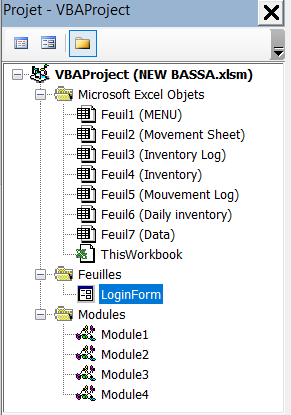
\includegraphics[width=0.4\textwidth]{Logic.png} % chemin de l'image
    \caption{Répartition du code}
    \label{fig:Répartition du code}
\end{figure}

\section{Le Formulaire de Connexion}
Le formulaire de connexion représente l'entrée principale de l'application, garantissant que l'accès est contrôlé et sécurisé. Plus qu'un simple écran de connexion, il incarne la première interaction de l'utilisateur avec l'application, posant les bases d'une expérience utilisateur sécurisée et fiable. Le formulaire est conçu pour être à la fois simple et efficace, tout en assurant une protection rigoureuse des données. En le plaçant au cœur de l'application, nous avons voulu souligner l'importance de la sécurité et de la confidentialité des informations, tout en offrant une transition fluide vers les autres fonctionnalités une fois l'accès autorisé.

\section{Mouvement sheet}
\subsection{movementCounters}
Le code présenté commence par la déclaration d'une variable nommée movementCounters, qui est définie comme un objet de type Scripting.Dictionary. Cette déclaration est typique dans les langages de programmation VBA (Visual Basic for Applications), utilisés couramment pour automatiser des tâches dans des applications telles qu'Excel.

\subsubsection{Définition et rôle de Scripting.Dictionary}
Scripting.Dictionary est une collection associative, ou un conteneur de paires clé-valeur. Contrairement aux tableaux traditionnels, où les éléments sont indexés par des entiers, un dictionnaire permet d'utiliser des clés de type chaîne de caractères ou d'autres types, ce qui offre une plus grande flexibilité pour accéder et manipuler les données. Dans le contexte d'un projet de gestion d'inventaire, par exemple, un dictionnaire pourrait être utilisé pour stocker les quantités de différents types de produits en utilisant les noms de produits comme clés.

\subsubsection{Utilisation de Scripting.Dictionary dans le Projet}
Dans le cadre de mon projet de stage, la variable movementCounters est utilisée pour suivre et gérer les mouvements des stocks au quotidien. Chaque type de produit (ou groupe de produits) est associé à une clé spécifique dans le dictionnaire. La valeur associée à chaque clé correspond au nombre de mouvements (entrées ou sorties) pour ce type de produit.

Cette approche permet de :
\begin{itemize}


\item Optimiser la gestion des données : Le dictionnaire permet un accès rapide et direct aux données des mouvements de chaque produit, sans avoir à parcourir une liste ou un tableau pour les retrouver.

\item Faciliter les mises à jour en temps réel : À chaque fois qu'un produit est déplacé (ajout ou retrait du stock), le dictionnaire est mis à jour instantanément, garantissant ainsi que les données sont toujours à jour.

\item Améliorer la flexibilité du code : La nature dynamique du dictionnaire permet d'ajouter ou de retirer des produits sans nécessiter de modifications majeures dans la structure du code. Cela est particulièrement utile dans un environnement de travail où les types de produits peuvent changer fréquemment.
\end{itemize}
\subsubsection{Avantages pour le Projet de Gestion des Stocks}
L'utilisation d'un Scripting.Dictionary pour suivre les mouvements de stocks présente plusieurs avantages :
\begin{itemize}


\item \textbf{Efficacité :} Le dictionnaire permet une gestion des mouvements plus rapide et plus efficace que les structures de données traditionnelles, car il offre un accès direct aux données via les clés.

\item \textbf{Réduction des erreurs :} Grâce à la nature associative du dictionnaire, le risque d'erreurs liées à l'accès aux données est réduit, car il n'y a pas de confusion possible entre les index numériques.

\item \textbf{Extensibilité :} Le code utilisant un dictionnaire est facilement extensible. Si de nouveaux types de produits sont ajoutés à l'inventaire, il suffit de les ajouter comme nouvelles clés dans le dictionnaire, sans nécessiter de restructuration du code existant.
\end{itemize}

En résumé, la déclaration de la variable movementCounters en tant que Scripting.Dictionary représente une approche puissante et flexible pour gérer les mouvements de stocks dans le cadre du projet de stage. Cette technique améliore non seulement la performance du code, mais aussi sa maintenabilité et sa robustesse, tout en garantissant une gestion précise et à jour des données d'inventaire.
\subsection{InitializeCounters}
La fonction \texttt{InitializeCounters}, écrite en VBA (Visual Basic for Applications), joue un rôle clé dans l'initialisation et la gestion des compteurs de mouvements de stock au sein de l'application de gestion d'inventaire que je développe dans le cadre de mon stage. Cette fonction est responsable de la création et de la configuration initiale d'un dictionnaire, \texttt{movementCounters}, qui est utilisé pour suivre les différents types de mouvements de produits au quotidien.

\subsubsection{Structure de la Fonction}
La fonction commence par la déclaration de la variable \texttt{movementCounters} en tant qu'objet de type \texttt{Scripting.Dictionary}. Ensuite, elle initialise ce dictionnaire en le remplissant avec des paires clé-valeur, où chaque clé représente un type spécifique de mouvement de stock, et la valeur associée est initialisée à zéro.

\subsubsection{Étapes d'Initialisation}
Voici un aperçu détaillé des étapes effectuées par la fonction :

-Création du Dictionnaire
Ce code initialise un objet Scripting.Dictionary en utilisant la méthode CreateObject. Cette instance de dictionnaire sera utilisée pour gérer les compteurs de mouvements dans l'application, permettant ainsi de stocker et de manipuler des données clés de manière efficace.
Cette ligne de code crée une instance du dictionnaire \texttt{movementCounters}. Le dictionnaire est un conteneur de données où chaque élément est constitué d'une paire clé-valeur. Ici, \texttt{CreateObject("Scripting.Dictionary")} est utilisé pour instancier un nouvel objet de type \texttt{Scripting.Dictionary}, qui servira à stocker les compteurs de différents types de mouvements de stock.

-Ajout des Clés et Initialisation des Valeurs
Ce code ajoute plusieurs éléments au dictionnaire movementCounters, avec chaque clé représentant un type spécifique de mouvement ou de transaction et chaque valeur initialisée à zéro. Cela permet de préparer le dictionnaire pour suivre et comptabiliser ces différents types de mouvements tout au long de l'application.

Chaque clé est ajoutée au dictionnaire \texttt{movementCounters} avec une valeur initiale de 0.

Chaque appel à la méthode \texttt{Add} du dictionnaire ajoute une nouvelle paire clé-valeur. Les clés sont des identifiants pour différents types de mouvements, et les valeurs associées sont initialisées à zéro, indiquant qu'aucun mouvement de ce type n'a encore été enregistré.

\paragraph{Description des Clés :}
\begin{itemize}
    \item \texttt{"TRFEMB"} (Transfert d'emballages) : Compte les mouvements de transfert des emballages entre différentes zones ou entités.
    \item \texttt{"EXPEMB"} (Expédition d'emballages) : Suivi des emballages qui sont expédiés en dehors du site.
    \item \texttt{"LIVPRD"} (Livraison de produits) : Comptabilise les livraisons de produits aux clients ou entre les sites.
    \item \texttt{"RCPPRD"} (Réception de produits) : Enregistre les réceptions de produits entrants sur le site.
    \item \texttt{"RCPEMB"} (Réception d'emballages) : Suivi des emballages reçus sur le site.
    \item \texttt{"RCPACC"} (Réception d'accessoires) : Compte les accessoires reçus en stock.
    \item \texttt{"EXPACC"} (Expédition d'accessoires) : Suivi des accessoires expédiés.
    \item \texttt{"TRFACC"} (Transfert d'accessoires) : Comptabilise les transferts d'accessoires entre les sites ou départements.
\end{itemize}

-Importance et Utilisation dans le Projet
La fonction \texttt{InitializeCounters} est essentielle pour garantir que tous les types de mouvements de produits sont correctement suivis dès le démarrage de l'application. En initialisant les valeurs à zéro, la fonction garantit que chaque compteur commence à une valeur neutre, prête à être incrémentée au fur et à mesure que des mouvements sont enregistrés.

Cette méthode d'initialisation assure également que le dictionnaire contient uniquement les types de mouvements pertinents pour l'application, évitant ainsi toute confusion ou erreur potentielle liée à des types de mouvements non pris en charge.

\subsubsection{Avantages de l'Approche Utilisée}
\begin{itemize}
    \item \textbf{Clarté et lisibilité du code :} L'utilisation d'un dictionnaire avec des clés explicites permet une gestion claire et lisible des différents types de mouvements. Cela rend le code facile à comprendre et à maintenir.
    \item \textbf{Facilité de mise à jour :} Si de nouveaux types de mouvements doivent être ajoutés à l'avenir, il suffit de les inclure dans la fonction \texttt{InitializeCounters}, sans avoir à restructurer l'ensemble du code.
    \item \textbf{Évolutivité :} Cette approche est évolutive et peut être facilement adaptée pour inclure de nouveaux types de mouvements ou pour être utilisée dans d'autres contextes de suivi des données.
\end{itemize}


En conclusion, la fonction \texttt{InitializeCounters} constitue une étape fondamentale dans l'initialisation de l'application de gestion des stocks développée durant mon stage. Elle permet de préparer efficacement le terrain pour la gestion des mouvements de produits, en s'assurant que chaque type de mouvement est correctement suivi dès le début. Cette fonction contribue ainsi de manière significative à la robustesse et à la fiabilité de l'application.

\subsection{ Worksheet Activate}
La fonction \texttt{Worksheet\_Activate} en VBA (Visual Basic for Applications) est un événement qui se déclenche automatiquement à chaque fois que la feuille de calcul associée est activée, c’est-à-dire lorsque l’utilisateur clique sur cette feuille ou y navigue depuis une autre feuille. Cette fonction est essentielle pour configurer et mettre à jour dynamiquement les validations de données sur certaines cellules, garantissant que l'utilisateur dispose d'options précises et pertinentes lors de la saisie de données.

\subsubsection{Structure et Rôle de la Fonction}

La fonction commence par la déclaration de plusieurs variables, dont \texttt{articles}, \texttt{categories}, et \texttt{FileType}, qui stockent des tableaux de chaînes de caractères. Ces tableaux sont ensuite utilisés pour créer des listes déroulantes dans des cellules spécifiques de la feuille de calcul, via la fonctionnalité de validation des données d'Excel.

\subsubsection{Déclaration des Variables}

articles : une variable qui sera utilisée pour stocker une collection ou un tableau d'articles.
rowNum : une variable de type Long destinée à stocker un numéro de ligne.
categories : une variable qui sera utilisée pour stocker une collection ou un tableau de catégories.
FileType : une variable qui sera utilisée pour stocker le type de fichier ou le format de données.


\begin{itemize}
    \item \texttt{articles} : Contient une liste des articles disponibles pour la sélection.
    \item \texttt{categories} : Stocke les différentes catégories auxquelles ces articles peuvent appartenir.
    \item \texttt{FileType} : Contient une liste des types de fichiers ou formulaires pertinents pour les enregistrements.
\end{itemize}

\subsubsection{Initialisation des Tableaux}

Ces tableaux sont utilisés pour stocker et organiser les catégories, les articles et les types de fichiers dans l'application.

Ces tableaux sont remplis avec des valeurs prédéfinies qui correspondent aux différentes options disponibles pour les utilisateurs lors de la saisie de données. Chaque tableau regroupe des éléments similaires pour simplifier l'organisation des options.

\subsubsection{Configuration des Listes de Validation de Données}

Le cœur de la fonction réside dans la création et la configuration des listes déroulantes pour certaines cellules à l'aide de la validation des données. Cela permet d'assurer que seules les valeurs valides peuvent être saisies par l'utilisateur dans ces cellules.

\textbf{Validation pour la Cellule L6 (Type de Fichier)}

Ce code configure la validation de données pour la cellule L6 dans Excel. Il supprime d'abord toute validation existante, puis ajoute une validation de liste en utilisant les valeurs du tableau FileType. La cellule affiche une liste déroulante pour la sélection, et les options de validation permettent de gérer les erreurs et de montrer des messages d'entrée si nécessaire.

Cette partie du code configure la cellule \texttt{L6} pour qu'elle affiche une liste déroulante contenant les éléments du tableau \texttt{FileType}. Avant de créer la validation, toute validation existante est supprimée pour éviter les conflits.

\textbf{Validation pour les Cellules G42 et G43 (Articles)}

Ce code configure la validation de données pour les cellules G42 et G43 dans Excel. Pour chaque cellule, il supprime toute validation précédente, puis ajoute une validation de liste en utilisant les valeurs du tableau articles. Les cellules affichent une liste déroulante pour la sélection, avec des options pour afficher des messages d'entrée et gérer les erreurs.

Les cellules \texttt{G42} et \texttt{G43} sont configurées de manière similaire à \texttt{L6}, mais cette fois en utilisant les \texttt{articles} comme options disponibles. Ceci est crucial pour garantir que seuls les articles valides peuvent être sélectionnés.

\textbf{Validation pour les Cellules H20 et L20 (Catégories)}
Ce code configure la validation de données pour les cellules H19 et L19 dans le formulaire actuel. Pour chaque cellule, il supprime d'abord toute validation existante, puis ajoute une validation de liste avec les valeurs du tableau categories. Les cellules afficheront une liste déroulante pour la sélection, avec des options pour afficher des messages d'entrée et gérer les erreurs.








Les cellules \texttt{H20} et \texttt{L20} sont également configurées pour afficher une liste déroulante des \texttt{catégories} disponibles. Cela permet aux utilisateurs de choisir facilement la catégorie appropriée lors de la saisie des données.

\subsubsection{Mise à Jour Dynamique des Colonnes}

Ce code itère sur les lignes de 42 à 80, appelant la fonction UpdateDColumn pour chaque numéro de ligne. Cela permet de mettre à jour les cellules de la colonne D pour chaque ligne dans cette plage.

Cette boucle \texttt{for} itère sur les lignes \texttt{42} à \texttt{80}, appelant une fonction (probablement définie ailleurs) nommée \texttt{UpdateDColumn}, qui met à jour dynamiquement les validations ou autres paramètres des cellules dans la colonne \texttt{D} pour les lignes spécifiées. Cela garantit que les validations sont actualisées en fonction des données actuelles ou des besoins spécifiques de chaque ligne.

\subsubsection{Appel de la Fonction \texttt{CreateDropDownListFromColumnM}}

Ce code appelle la fonction CreateDropDownListFromColumnM, qui est chargée de créer une liste déroulante en utilisant les valeurs de la colonne M.
Cette dernière ligne appelle une autre fonction nommée \texttt{CreateDropDownListFromColumnM}, qui est chargée de créer une liste déroulante basée sur les valeurs présentes dans la colonne \texttt{M}. Cette fonctionnalité est utile pour dynamiser davantage la feuille de calcul et assurer une meilleure flexibilité dans la gestion des données.


\subsection{IncrementCounter}
La fonction \texttt{IncrementCounter} en VBA (Visual Basic for Applications) est une procédure essentielle pour la gestion des compteurs de mouvements dans le cadre d'un projet de suivi d'inventaire. Son rôle principal est d'incrémenter un compteur spécifique associé à un type de mouvement donné. Cette fonction est conçue pour être à la fois robuste et adaptable, en veillant à ce que les compteurs soient correctement initialisés avant d'être modifiés.

\subsubsection{Structure de la Fonction}
La fonction \texttt{IncrementCounter} prend un paramètre, \texttt{shortName}, qui correspond à une clé spécifique dans le dictionnaire \texttt{movementCounters}. Ce dictionnaire contient les différents types de mouvements de stock et leurs compteurs respectifs.

\textbf{Vérification de l'Initialisation du Dictionnaire}

Ce code vérifie si l'objet movementCounters est vide ou non initialisé. Si c'est le cas, il appelle la fonction InitializeCounters pour initialiser les compteurs de mouvements.

La première étape de la fonction consiste à vérifier si le dictionnaire \texttt{movementCounters} a été initialisé. Si le dictionnaire n'est pas encore créé (c'est-à-dire qu'il est \texttt{Nothing}), la fonction appelle \texttt{InitializeCounters} pour l'initialiser. Cela garantit que le dictionnaire est toujours disponible et prêt à être utilisé, évitant ainsi toute erreur liée à l'absence de ce dernier.

\textbf{Robustesse} : Cette vérification rend la fonction plus robuste en s'assurant que l'objet \texttt{movementCounters} est correctement configuré avant d'essayer de l'utiliser.

\textbf{Prévention des erreurs} : Cela évite des erreurs potentielles qui pourraient survenir si l'utilisateur tente d'incrémenter un compteur sans que le dictionnaire ne soit initialisé.



\textbf{Incrémentation du Compteur}


Ce code vérifie si la clé shortName existe dans l'objet movementCounters. Si la clé est présente, il incrémente la valeur associée à cette clé de 1.

Après s'être assuré que le dictionnaire est initialisé, la fonction vérifie si la clé \texttt{shortName} existe dans le dictionnaire. Si c'est le cas, elle incrémente la valeur associée à cette clé de 1.

\textbf{Vérification de l'existence} : En vérifiant l'existence de la clé avec \texttt{movementCounters.Exists(shortName)}, la fonction assure que seules les clés valides sont manipulées. Cela renforce la sécurité et la fiabilité du code en évitant les erreurs qui pourraient résulter de tentatives d'accès à des clés inexistantes.

\textbf{Incrémentation} : Si la clé existe, le compteur associé est incrémenté de 1, ce qui correspond à l'enregistrement d'un nouveau mouvement de ce type. Cette opération est au cœur de la gestion des mouvements de stock, permettant de maintenir un suivi précis et à jour des différents types de mouvements.

\subsubsection{Importance et Utilisation dans le Projet}
La fonction \texttt{IncrementCounter} est cruciale dans le cadre du projet de gestion d'inventaire que nous développons. Chaque fois qu'un mouvement de stock est enregistré, cette fonction est appelée pour mettre à jour le compteur correspondant. Cela permet de suivre en temps réel le nombre de mouvements pour chaque type de produit ou d'article.

\textbf{Suivi en temps réel} : En permettant l'incrémentation immédiate des compteurs, la fonction contribue à un suivi en temps réel des opérations, ce qui est essentiel pour une gestion efficace des stocks.

\textbf{Flexibilité} : L'usage de la fonction \texttt{InitializeCounters} pour l'initialisation permet à la fonction \texttt{IncrementCounter} d'être utilisée à tout moment, même si le dictionnaire n'était pas encore prêt. Cela rend le système flexible et capable de s'adapter à différents scénarios d'utilisation.

\subsubsection{Avantages de l'Approche Utilisée}
\textbf{Sécurité} : La vérification de l'initialisation et de l'existence des clés garantit que la fonction fonctionne toujours dans un état valide, réduisant les risques d'erreurs.

\textbf{Modularité} : La fonction est conçue de manière modulaire, ce qui permet une réutilisation facile dans d'autres parties du code ou dans d'autres projets nécessitant une gestion similaire des compteurs.

\textbf{Simplicité} : L'approche simple et directe de l'incrémentation rend la fonction facile à comprendre et à maintenir.


\subsection{SetValidationList}
La fonction \texttt{SetValidationList} en VBA (Visual Basic for Applications) est conçue pour configurer une liste de validation de données sur une feuille Excel spécifique. Cette fonctionnalité est cruciale pour garantir que les utilisateurs sélectionnent des options prédéfinies dans une cellule donnée, ce qui réduit les erreurs d'entrée et améliore la cohérence des données. Dans le cadre de mon projet de stage, cette fonction est utilisée pour assurer une gestion précise et contrôlée des types de mouvements de stock.

\subsubsection{Structure de la Fonction}
La fonction \texttt{SetValidationList} configure une liste déroulante dans une cellule spécifique en utilisant une liste d'options prédéfinies. Elle commence par définir les variables nécessaires, puis procède à la création de la liste de validation de données.

\textbf{a. Définition des Variables}
Ce code déclare trois variables dans VBA :

ws : une variable destinée à contenir une référence à une feuille de calcul (Worksheet).
validationArray : une variable qui sera utilisée pour stocker un tableau de données pour la validation.
nameMapping : une variable qui sera utilisée pour stocker un tableau de correspondance des noms.

Les variables \texttt{ws}, \texttt{validationArray}, et \texttt{nameMapping} sont initialisées pour stocker la feuille de calcul cible, le tableau de validation, et le mappage des noms respectivement.

\begin{itemize}
    \item \texttt{ws} : Représente la feuille de calcul où la validation sera appliquée.
    \item \texttt{validationArray} : Contient les options de validation qui seront affichées dans la liste déroulante.
    \item \texttt{nameMapping} : Un tableau à deux dimensions qui associe les descriptions textuelles des mouvements avec leurs abréviations correspondantes.
\end{itemize}
Ce code initialise un tableau à deux dimensions nommé nameMapping. Chaque élément du tableau est un sous-tableau contenant une paire de valeurs : une description textuelle d'un type de mouvement ou de transaction et son code abrégé associé. Ces paires sont utilisées pour établir un mappage entre les noms complets et leurs abréviations correspondantes.

Le tableau \texttt{nameMapping} associe les descriptions textuelles des mouvements de stock à leurs abréviations respectives. Ce mappage permet de garantir que seules les options valides sont disponibles pour la sélection, ce qui facilite l'identification rapide des types de mouvements dans la gestion des stocks.

\textbf{c. Sélection de la Feuille de Calcul}

Ce code assigne à la variable ws une référence à la feuille de calcul nommée "Movement Sheet" dans le classeur actif.

La feuille de calcul où la validation sera appliquée est définie en utilisant \texttt{Set ws}. Ici, la feuille s'appelle "Movement Sheet". Si la feuille spécifiée n'existe pas, un message d'erreur s'affiche et la fonction s'arrête pour éviter des erreurs d'exécution.

\textbf{d. Création de la Liste de Validation}
Ce code transpose la première colonne du tableau nameMapping et assigne le résultat à la variable validationArray. Cela permet de créer un tableau contenant uniquement les descriptions des types de mouvements ou de transactions à partir du mappage des noms.

L'étape suivante consiste à créer un tableau unidimensionnel, \texttt{validationArray}, qui contient les descriptions textuelles des mouvements (la première colonne de \texttt{nameMapping}). Ce tableau est ensuite utilisé pour générer la liste de validation.

\textbf{e. Application de la Validation de Données}
Ce code configure la validation des données pour la cellule L7 dans la feuille de calcul ws. Il supprime d'abord toute validation existante, puis ajoute une validation de liste en utilisant les valeurs du tableau validationArray. La cellule affichera une liste déroulante avec les options spécifiées, et les paramètres de validation permettent de gérer les erreurs et d'afficher des messages d'entrée si nécessaire.

La validation de données est appliquée à la cellule \texttt{L7} de la feuille spécifiée. La validation de données est d'abord supprimée (s'il en existe), puis une nouvelle validation de type \texttt{xlValidateList} est ajoutée, permettant à l'utilisateur de sélectionner uniquement les options définies dans \texttt{validationArray}.

\begin{itemize}
    \item \textbf{Effacement des validations existantes} : Le code commence par supprimer toute validation déjà présente dans la cellule, ce qui assure que seule la nouvelle validation définie sera en place.
    \item \textbf{Ajout de la liste de validation} : La liste déroulante est ensuite ajoutée avec les options définies, ce qui facilite la sélection correcte des types de mouvements.
\end{itemize}

\subsubsection{Importance et Utilisation dans le Projet}
La fonction \texttt{SetValidationList} est essentielle pour la gestion des mouvements de stock dans le cadre de mon projet de stage. En limitant les choix possibles à une liste prédéfinie, cette fonction réduit les risques d'erreurs lors de la saisie des données et assure la cohérence des enregistrements.

\begin{itemize}
    \item \textbf{Réduction des erreurs} : En utilisant des listes déroulantes, la fonction limite les choix possibles, ce qui réduit considérablement les erreurs de saisie.
    \item \textbf{Cohérence des données} : Les options étant standardisées, toutes les entrées pour un type de mouvement spécifique seront identiques, ce qui améliore la qualité des données.
    \item \textbf{Facilité d'utilisation} : Les utilisateurs peuvent facilement sélectionner le bon type de mouvement grâce à la liste déroulante, rendant le processus plus rapide et plus intuitif.
\end{itemize}

\subsubsection{Avantages de l'Approche Utilisée}
\begin{itemize}
    \item \textbf{Robustesse} : La vérification de l'existence de la feuille de calcul avant d'appliquer la validation garantit que le code ne génère pas d'erreurs inattendues.
    \item \textbf{Flexibilité} : Le mappage des noms dans un tableau permet d'ajouter facilement de nouveaux types de mouvements ou de modifier les existants sans avoir à changer le code principal.
    \item \textbf{Simplicité et Maintenabilité} : Le code est écrit de manière à être facilement compréhensible et modifiable, ce qui est crucial pour la maintenance future.
\end{itemize}


\subsection{Worksheet Change}
La fonction \texttt{Worksheet\_Change} est un gestionnaire d'événements dans VBA qui se déclenche automatiquement lorsqu'une modification est apportée à une cellule de la feuille de calcul. Cette fonction est un élément clé dans la gestion dynamique des données de l'inventaire au sein du projet. Voici une explication détaillée de son fonctionnement.

\subsubsection{Objectif Principal}
La fonction \texttt{Worksheet\_Change} surveille et gère les modifications apportées à certaines cellules spécifiques de la feuille de calcul. Elle effectue diverses actions basées sur ces changements, telles que la mise à jour des listes de validation, l'incrémentation des compteurs de mouvement, et l'affichage de messages d'avertissement lorsque des conditions spécifiques sont remplies.

\subsubsection{Détection des Modifications}
La fonction commence par vérifier si les modifications se sont produites dans des plages spécifiques, telles que les colonnes G, H, et L, et prend des mesures en conséquence :

\begin{itemize}
    \item \textbf{Colonne G42} : Lorsque des changements sont détectés dans cette plage, la fonction appelle \texttt{UpdateDColumn} pour mettre à jour les données de la colonne D correspondant à la ligne modifiée.
    
    \item \textbf{Cellule L7} : Si une modification est apportée à cette cellule, la fonction récupère la valeur sélectionnée, la compare à une liste prédéfinie de types de mouvements (nom court) et incrémente un compteur spécifique via la fonction \texttt{IncrementCounter}. Le compteur mis à jour est affiché dans la cellule L8.
    
    \item \textbf{Cellules H19 et L19} : Toute modification dans ces cellules déclenche la mise à jour des cellules H20 et L20, respectivement, en appelant des fonctions dédiées \texttt{UpdateH20BasedOnL19} et \texttt{UpdateL20BasedOnL19}.
    
    \item \textbf{Colonne Q (à partir de Q21)} : Lorsque des modifications sont apportées dans cette colonne, les cellules correspondantes dans les colonnes R et S sont effacées, et la fonction \texttt{CheckQAndRetrieveEmailAndPost} est appelée pour mettre à jour ces colonnes en fonction des nouvelles données saisies dans Q.
\end{itemize}

\subsubsection{Gestion des Avertissements}
La fonction inclut également une vérification pour s'assurer que les cellules L20 et H20 ne contiennent pas les mêmes valeurs, ce qui pourrait entraîner des incohérences dans les données d'inventaire (par exemple, la destination ne peut pas être identique à la source). Si une telle situation est détectée, un message d'avertissement est affiché, et la cellule L20 est effacée.


\subsection{UpdateDColumn}
La fonction \texttt{UpdateDColumn} est un sous-programme en VBA (Visual Basic for Applications) qui a été développée pour gérer la validation dynamique des données dans une feuille de calcul Excel intitulée \textit{Movement Sheet}. Cette fonction est spécifiquement conçue pour mettre à jour la validation de données dans une cellule de la colonne H en fonction de la valeur sélectionnée dans la colonne G pour une ligne donnée. Voici une explication détaillée de chaque étape de la fonction, accompagnée de la logique sous-jacente et de son utilité dans le contexte du projet.

\subsubsection{Objectif de la Fonction}
L'objectif principal de \texttt{UpdateDColumn} est de garantir que les options disponibles pour une cellule donnée dans la colonne H (la colonne où les choix d'emballage sont effectués) correspondent précisément au type de produit ou d'emballage sélectionné dans la colonne G. Cette validation dynamique améliore l'intégrité des données et réduit le risque d'erreurs de saisie en limitant les choix possibles aux options pertinentes pour le produit ou l'emballage en question.

\subsubsection{Explication du Code}
\textbf{Initialisation des Variables}
La fonction commence par déclarer et initialiser plusieurs variables :

\begin{itemize}
    \item \textbf{ws} : représente la feuille de calcul \textit{Movement Sheet}.
    \item \textbf{selectedValue} : stocke la valeur sélectionnée dans la colonne G.
    \item \textbf{emballageOptions} : un tableau qui contiendra les options spécifiques de validation pour la cellule de la colonne H.
    \item \textbf{validationList} : une chaîne de caractères qui contient les options de validation sous forme de liste séparée par des virgules.
    \item \textbf{previousValue} : stocke la valeur précédente de la colonne H pour vérifier si elle doit être réinitialisée.
\end{itemize}

\textbf{Validation de la Plage de Lignes}
La fonction vérifie si le numéro de ligne (\texttt{rowNum}) passé en paramètre est compris entre 42 et 80. Si ce n'est pas le cas, la fonction se termine immédiatement avec \texttt{Exit Sub} pour éviter des erreurs de traitement en dehors de la plage prévue.

\textbf{Récupération des Valeurs Précédentes et Sélectionnées}
Le programme récupère la valeur précédente dans la colonne H (\texttt{previousValue}) et la valeur sélectionnée dans la colonne G (\texttt{selectedValue}) pour la ligne spécifiée. Si la valeur sélectionnée diffère de la valeur précédente, la cellule de la colonne H est réinitialisée (son contenu est effacé).

\textbf{Détermination des Options d'Emballage}
La fonction utilise une structure \texttt{Select Case} pour déterminer les options d'emballage spécifiques à afficher en fonction de la valeur sélectionnée dans la colonne G. Chaque cas correspond à un type spécifique de produit ou d'emballage, et le tableau \texttt{emballageOptions} est rempli avec les choix appropriés. Par exemple :

\begin{itemize}
    \item Pour une \textit{Bouteille 6KG}, les options incluent \textit{Bouteille pleine}, \textit{Bouteille vide en service}, etc.
    \item Pour un \textit{Robinet}, les options sont \textit{Robinet en bon état} et \textit{Robinet défectueux}.
\end{itemize}

Si l'option sélectionnée ne nécessite qu'une seule valeur (par exemple \textit{Ecrou}), cette valeur est automatiquement définie dans la colonne H.

\textbf{Création et Application de la Liste de Validation}
Si le tableau \texttt{emballageOptions} contient des valeurs, celles-ci sont converties en une liste séparée par des virgules (\texttt{validationList}). La validation de données de la cellule de la colonne H est ensuite mise à jour pour refléter cette liste. Toute validation existante est d'abord supprimée avant d'appliquer la nouvelle liste pour éviter les conflits ou les erreurs.

\textbf{Gestion des Cas où la Liste est Vide}
Si la liste de validation est vide, la fonction imprime un message de débogage indiquant qu'aucune option n'a été trouvée pour la valeur sélectionnée. Cela permet de détecter et de corriger des erreurs potentielles lors du développement.


\subsection{UpdateH20BasedOnL19}
La fonction \texttt{UpdateH20BasedOnL19} est une procédure VBA (Visual Basic for Applications) conçue pour gérer dynamiquement la validation des données dans une cellule spécifique d'une feuille de calcul Excel, en fonction de la valeur sélectionnée dans une autre cellule. Plus précisément, cette fonction met à jour la validation de données dans la cellule H20 de la feuille de calcul \textit{Movement Sheet} en fonction de la valeur choisie dans la cellule H19, en appliquant des listes nommées appropriées.

\subsubsection{Objectif de la Fonction}
L'objectif principal de la fonction \texttt{UpdateH20BasedOnL19} est d'adapter la liste déroulante des options disponibles dans la cellule H20 selon le type de catégorie sélectionné dans la cellule H19. Cela garantit que les utilisateurs ont accès uniquement aux options pertinentes et appropriées, ce qui réduit les erreurs de saisie et renforce l'intégrité des données.

\subsubsection{Description des Étapes du Code}
\textbf{Initialisation des Variables}
La fonction commence par déclarer et initialiser plusieurs variables :

\begin{itemize}
    \item \textbf{ws} : variable de type \texttt{Worksheet} qui fait référence à la feuille de calcul active nommée \textit{Movement Sheet}.
    \item \textbf{selectedValue} : variable de type \texttt{String} qui stocke la valeur sélectionnée dans la cellule H19.
    \item \textbf{namedRange} : variable de type \texttt{String} qui contient le nom de la plage nommée à utiliser pour la validation de la cellule H20.
\end{itemize}

\subsubsection{Récupération de la Valeur Sélectionnée}
La fonction récupère la valeur actuelle de la cellule H19 dans la variable \texttt{selectedValue}. Cette valeur détermine quelles options seront disponibles pour la cellule H20.

\subsubsection{Suppression de la Validation Existante}
Avant de mettre à jour la validation des données dans H20, toute validation existante est supprimée pour éviter les conflits. Cela est accompli avec la méthode \texttt{Validation.Delete}.

\subsubsection{Détermination de la Plage Nommée Basée sur la Valeur Sélectionnée}
Une structure \texttt{Select Case} est utilisée pour associer la valeur sélectionnée dans H19 à une plage nommée spécifique :

\begin{itemize}
    \item Par exemple, si la valeur est \textit{StationDeService}, la plage nommée \textit{StationSRV} est attribuée à \texttt{namedRange}.
    \item De même, d'autres valeurs comme \textit{ClientB2B}, \textit{MagasinGPL}, \textit{DépôtGPL}, \textit{Fournisseur}, et \textit{Prestataire} sont mappées à leurs plages nommées respectives.
\end{itemize}

Si la valeur sélectionnée dans H19 ne correspond à aucun des cas spécifiés, \texttt{namedRange} reste vide.

\subsubsection{Application de la Validation de Données}
Si une plage nommée valide est déterminée, la fonction vérifie d'abord l'existence de cette plage pour éviter les erreurs. Si la plage existe, une validation de données est ajoutée à la cellule H20. Cette validation utilise la plage nommée déterminée précédemment comme source pour la liste déroulante.

La validation est configurée pour permettre la sélection directe dans la cellule (grâce à \texttt{InCellDropdown = True}) et pour afficher des messages d'erreur et d'entrée le cas échéant.

\subsubsection{Prise en Compte des Cas avec une Seule Option}
Si la plage nommée ne contient qu'une seule cellule, cette valeur unique est automatiquement définie dans H20. Si la plage contient plusieurs valeurs, H20 est laissée vide pour permettre à l'utilisateur de faire un choix.

\subsubsection{Gestion des Erreurs et Messages}
La fonction inclut une gestion d'erreurs simple pour alerter l'utilisateur si la plage nommée spécifiée n'existe pas. Un message d'avertissement s'affiche alors pour informer de cette situation. Si \texttt{namedRange} est vide, la cellule H20 est simplement réinitialisée à une valeur vide.


\subsection{UpdateL20BasedOnL19}
La fonction \texttt{UpdateL20BasedOnL19} est un sous-programme VBA (Visual Basic for Applications) conçu pour gérer dynamiquement la validation des données dans une cellule spécifique d'une feuille de calcul Excel, en fonction de la valeur sélectionnée dans une autre cellule. Plus précisément, cette fonction met à jour la validation des données dans la cellule L20 de la feuille de calcul \textit{Movement Sheet} en fonction de la valeur choisie dans la cellule L19, en appliquant des plages nommées appropriées.

\subsubsection{Objectif de la Fonction}
L'objectif principal de cette fonction est d'adapter la liste déroulante des options disponibles dans la cellule L20 selon le type de catégorie sélectionné dans la cellule L19. Cela permet de s'assurer que les utilisateurs n'ont accès qu'aux options pertinentes et appropriées, réduisant ainsi les erreurs de saisie et améliorant l'intégrité des données.

\subsubsection{Étapes Clés du Code}

\textbf{Initialisation des Variables}
La fonction commence par déclarer et initialiser plusieurs variables :

\begin{itemize}
    \item \textbf{ws} : de type \texttt{Worksheet}, elle fait référence à la feuille de calcul active nommée \textit{Movement Sheet}.
    \item \textbf{selectedValue} : de type \texttt{String}, elle stocke la valeur sélectionnée dans la cellule L19.
    \item \textbf{namedRange} : de type \texttt{String}, elle contient le nom de la plage nommée à utiliser pour la validation des données dans la cellule L20.
\end{itemize}

\subsubsection{Récupération de la Valeur Sélectionnée}
La fonction récupère la valeur actuelle de la cellule L19 dans la variable \texttt{selectedValue}. Cette valeur détermine quelles options seront disponibles pour la cellule L20.

\subsubsection{Suppression de la Validation Existante}
Avant de mettre à jour la validation des données dans L20, toute validation existante est supprimée à l'aide de la méthode \texttt{Validation.Delete}, garantissant ainsi que la nouvelle validation sera appliquée sans conflit.

\subsubsection{Détermination de la Plage Nommée Basée sur la Valeur Sélectionnée}
Une structure \texttt{Select Case} est utilisée pour associer la valeur sélectionnée dans L19 à une plage nommée spécifique :

\begin{itemize}
    \item Par exemple, si la valeur est \textit{StationDeService}, la plage nommée \textit{StationSRV} est attribuée à \texttt{namedRange}.
    \item D'autres valeurs comme \textit{ClientB2B}, \textit{MagasinGPL}, \textit{DépôtGPL}, \textit{Fournisseur}, et \textit{Prestataire} sont mappées à leurs plages nommées respectives.
\end{itemize}

Si la valeur sélectionnée dans L19 ne correspond à aucun des cas spécifiés, \texttt{namedRange} reste vide, ce qui signifie qu'aucune validation spécifique ne sera appliquée.

\subsubsection{Application de la Validation de Données}
Si une plage nommée valide est déterminée, la fonction vérifie d'abord l'existence de cette plage pour éviter les erreurs. Si la plage existe, une validation de données est ajoutée à la cellule L20, utilisant la plage nommée déterminée précédemment comme source pour la liste déroulante. La validation est configurée pour permettre la sélection directe dans la cellule, ainsi que pour afficher des messages d'entrée et des erreurs si nécessaire.

\subsection{Gestion des Cas avec une Seule Option}
Si la plage nommée ne contient qu'une seule cellule, cette valeur unique est automatiquement définie dans L20. Si la plage contient plusieurs valeurs, L20 est laissée vide pour permettre à l'utilisateur de faire un choix parmi les options disponibles.

\subsection{Gestion des Erreurs et Messages}
La fonction inclut une gestion d'erreurs simple pour alerter l'utilisateur si la plage nommée spécifiée n'existe pas. Un message d'avertissement s'affiche alors pour informer l'utilisateur de cette situation. Si \texttt{namedRange} est vide, la cellule L20 est simplement réinitialisée à une valeur vide.
\section{Inventory}
\subsection{Workbook Open}

La fonction \texttt{Workbook\_Open} est un événement déclenché automatiquement à chaque fois que le classeur Excel est ouvert. Ce sous-programme VBA (Visual Basic for Applications) est conçu pour définir des valeurs par défaut dans certaines cellules spécifiques de la feuille de calcul \texttt{Inventory} lorsque le classeur est ouvert. Cette automatisation permet de préparer le classeur avec des données prédéfinies sans nécessiter d'interaction manuelle de la part de l'utilisateur.

\subsubsection{Objectif de la Fonction}

L'objectif principal de la fonction \texttt{Workbook\_Open} est de garantir que certaines cellules dans la feuille de calcul \texttt{Inventory} sont initialisées avec des valeurs spécifiques à chaque ouverture du classeur. Cela assure une cohérence des données et permet aux utilisateurs de commencer avec des informations de base déjà renseignées, facilitant ainsi la saisie et l'analyse ultérieures.

\subsubsection{Description des Étapes du Code}

\textbf{Déclaration de l'Événement \texttt{Workbook\_Open}}

Le sous-programme est défini comme \texttt{Private Sub Workbook\_Open()}, ce qui signifie qu'il s'exécute automatiquement lorsque le classeur est ouvert, sans qu'il soit nécessaire de l'exécuter manuellement.

\subsubsection{Définition de la Feuille de Calcul}

La fonction utilise l'objet \texttt{ThisWorkbook} pour accéder au classeur actif et à la feuille de calcul spécifiée. La feuille de calcul \texttt{Inventory} est ciblée par le code suivant :

Ce code fait référence à la feuille de calcul nommée "Inventory" dans le classeur actif, permettant d'effectuer des opérations ou de manipuler des données spécifiques sur cette feuille.


Cela permet d'appliquer les modifications uniquement à cette feuille de calcul spécifique.

\subsubsection{Initialisation des Cellules}

Les valeurs suivantes sont définies pour certaines cellules de la feuille \texttt{Inventory} :

\begin{itemize}
    \item Cellule B8 : La valeur est définie comme une chaîne vide \texttt{""}. Cette initialisation peut être utilisée pour réinitialiser ou nettoyer la cellule à chaque ouverture du classeur.
    \item Cellule E8 : La valeur est également définie comme une chaîne vide \texttt{""}, de la même manière que pour la cellule B8.
    \item Cellule E7 : La valeur est définie sur la date actuelle, obtenue par la fonction \texttt{Date}. Cela insère automatiquement la date du jour dans la cellule E7.
    \item Cellule B7 : La valeur est également définie sur la date actuelle avec la même fonction \texttt{Date}, insérant ainsi la date du jour dans la cellule B7.
\end{itemize}

Ces initialisations sont réalisées dans le bloc \texttt{With ... End With} pour simplifier le code et améliorer sa lisibilité.

\subsubsection{Terminaison de l'Événement}

Le bloc \texttt{With ... End With} est fermé pour terminer la section de code qui modifie les cellules de la feuille \texttt{Inventory}.
\subsection{Worksheet Change}

La fonction \texttt{Worksheet\_Change} est un événement VBA qui se déclenche automatiquement chaque fois qu'une modification est apportée à la feuille de calcul. Cette fonction est conçue pour gérer les modifications spécifiques apportées à certaines cellules et appliquer des règles de validation des données en conséquence. Voici une explication détaillée du fonctionnement et des objectifs de cette fonction.

\subsubsection{Objectif de la Fonction}

L'objectif principal de la fonction \texttt{Worksheet\_Change} est de gérer les changements dans les cellules clés de la feuille de calcul et d'appliquer des validations appropriées. Plus précisément, cette fonction :

\begin{itemize}
    \item Valide les dates lorsqu'elles sont modifiées dans certaines cellules.
    \item Met à jour la liste de validation des données dans une cellule en fonction de la valeur sélectionnée dans une autre cellule.
\end{itemize}

\subsubsection{Description des Étapes du Code}

\textbf{Déclaration des Variables}

La fonction commence par déclarer deux variables :

\begin{itemize}
    \item \texttt{selected\_lpg} : une variable de type \texttt{String} qui stocke la valeur sélectionnée dans la cellule \texttt{B8}.
    \item \texttt{magasins} : une variable de type \texttt{Variant} qui est utilisée pour stocker les options de validation des données à appliquer dans la cellule \texttt{E8}.
\end{itemize}

\subsubsection{Gestion des Modifications dans les Cellules \texttt{B7} et \texttt{E7}}

Le premier bloc de code vérifie si la modification concerne les cellules \texttt{B7} ou \texttt{E7} :

Ce code vérifie si la cellule modifiée (Target) se trouve dans les plages B7 ou E7. Si c'est le cas, il appelle la fonction ValidateDatesInput pour valider les dates saisies. Si la validation échoue, les modifications sont annulées en utilisant Application.Undo.


\begin{itemize}
    \item \textbf{Intersection des Cellules Modifiées} : Le code utilise la méthode \texttt{Intersect} pour déterminer si les cellules modifiées se trouvent dans la plage \texttt{B7} ou \texttt{E7}.
    \item \textbf{Validation des Dates} : Si les modifications concernent ces cellules, la fonction \texttt{ValidateDatesInput} est appelée pour vérifier la validité des dates saisies. Si les dates ne sont pas valides, les modifications sont annulées à l'aide de \texttt{Application.Undo}.
\end{itemize}

\subsubsection{Gestion des Modifications dans la Cellule \texttt{B8}}

Le deuxième bloc de code gère les modifications apportées à la cellule \texttt{B8} :

Ce code vérifie si la cellule modifiée est B8. Si c'est le cas, il récupère la valeur de B8 et réinitialise la cellule E8. En fonction de la valeur sélectionnée dans B8, il détermine les options spécifiques à afficher dans la cellule E8 en utilisant un tableau prédéfini de magasins. Ensuite, il configure la validation des données pour E8, en créant une liste déroulante avec les options appropriées et en supprimant toute validation existante.

\begin{itemize}
    \item \textbf{Modification de \texttt{B8}} : Si une modification est apportée à la cellule \texttt{B8}, la fonction récupère la valeur sélectionnée et la stocke dans \texttt{selected\_lpg}.
    \item \textbf{Réinitialisation de \texttt{E8}} : La cellule \texttt{E8} est vidée pour préparer l'application de la nouvelle liste de validation.
    \item \textbf{Détermination des Options de Magasins} : Selon la valeur sélectionnée dans \texttt{B8}, une liste spécifique d'options est assignée à \texttt{magasins} à l'aide d'une structure \texttt{Select Case}.
    \item \textbf{Application de la Validation des Données} : La validation des données est configurée pour la cellule \texttt{E8} avec les options déterminées. Toute validation existante est d'abord supprimée avec \texttt{.Delete}, puis une nouvelle validation de liste est ajoutée. La liste déroulante dans \texttt{E8} est mise à jour pour refléter les options appropriées.
\end{itemize}
\subsection{Worksheet Activate}

La fonction \texttt{Worksheet\_Activate} est un événement VBA qui se déclenche automatiquement chaque fois que la feuille de calcul devient active, c'est-à-dire lorsqu'un utilisateur sélectionne ou passe à cette feuille dans le classeur Excel. Cette fonction est utilisée pour configurer des éléments de la feuille de calcul en fonction de l'activation de la feuille. Voici une explication détaillée du fonctionnement et des objectifs de cette fonction.

\subsubsection{Objectif de la Fonction}

L'objectif de la fonction \texttt{Worksheet\_Activate} est de préparer la feuille de calcul en définissant une liste déroulante pour une cellule spécifique chaque fois que la feuille devient active. Plus précisément, cette fonction configure une liste déroulante dans la cellule \texttt{B8}, permettant aux utilisateurs de choisir parmi une liste prédéfinie d'options.

\subsubsection{Description des Étapes du Code}

\textbf{Déclaration de la Variable}

La fonction commence par déclarer une variable :

\begin{itemize}
    \item \texttt{LPGS} : une variable de type \texttt{Variant} qui est utilisée pour stocker un tableau des options disponibles pour la liste déroulante.
\end{itemize}

\subsubsection{Définition des Options de Liste}

Le tableau \texttt{LPGS} est initialisé avec les valeurs suivantes :

Ce code initialise un tableau nommé LPGS contenant une liste de villes ou sites : "BASSA", "YAOUNDE", "BAFOUSSAM", "BERTOUA", et "GAROUA".

Ces valeurs représentent les différentes options disponibles pour la liste déroulante, correspondant à différents sites ou emplacements.

\subsubsection{Configuration de la Liste Déroulante}

La fonction configure ensuite la liste déroulante pour la cellule \texttt{B8} de la feuille de calcul active :


Ce code configure la validation des données pour la cellule B8. Il supprime d'abord toute validation existante, puis ajoute une validation de liste utilisant les valeurs du tableau LPGS. La cellule B8 affichera une liste déroulante avec ces options, permettant à l'utilisateur de sélectionner une valeur parmi les choix disponibles. Les paramètres de validation permettent également d'afficher des messages d'entrée et de gérer les erreurs.

\begin{itemize}
    \item \textbf{Suppression de la Validation Existante} : La méthode \texttt{.Delete} est utilisée pour supprimer toute validation des données existante dans la cellule \texttt{B8}. Cela garantit que la nouvelle liste déroulante remplace toute configuration précédente.
    \item \textbf{Ajout de la Nouvelle Validation} : La méthode \texttt{.Add} est utilisée pour créer une nouvelle validation des données. Le type de validation est défini comme \texttt{xlValidateList}, ce qui indique que la cellule contiendra une liste déroulante.
    \item \textbf{Configuration de la Liste Déroulante} : La liste des options est fournie via \texttt{Formula1:=Join(LPGS, ",")}. La fonction \texttt{Join} convertit le tableau \texttt{LPGS} en une chaîne de texte séparée par des virgules, ce qui est requis pour la validation de liste dans Excel.
    \item \textbf{Paramètres Additionnels} : Les propriétés \texttt{.IgnoreBlank}, \texttt{.InCellDropdown}, \texttt{.ShowInput}, et \texttt{.ShowError} sont configurées pour permettre une liste déroulante dans la cellule, ignorer les entrées vides, afficher un message d'entrée et afficher un message d'erreur si nécessaire.
\end{itemize}
\section{mouvement log}
\subsection{ExportSheetAsPDF}

La fonction \texttt{ExportSheetAsPDF} est une macro VBA conçue pour exporter une feuille de calcul Excel en tant que fichier PDF. Cette fonctionnalité est particulièrement utile pour partager ou archiver des données dans un format universel et lisible, tout en préservant la mise en page et la présentation de la feuille de calcul. Voici une explication détaillée du fonctionnement de cette fonction, étape par étape.

\subsubsection{Objectif de la Fonction}

L'objectif principal de la fonction \texttt{ExportSheetAsPDF} est de sauvegarder une feuille de calcul spécifique d'un classeur Excel en tant que fichier PDF sur le bureau de l'utilisateur. La fonction configure la mise en page de la feuille, définit les zones d'impression et exporte le document au format PDF avec des paramètres de qualité spécifiés.

\subsubsection{Description des Étapes du Code}

\paragraph{Déclaration des Variables}

La fonction commence par déclarer deux variables :

\begin{itemize}
    \item \texttt{ws} : Une variable de type \texttt{Worksheet} pour représenter la feuille de calcul à exporter.
    \item \texttt{pdfPath} : Une variable de type \texttt{String} pour stocker le chemin du fichier PDF de destination.
\end{itemize}

\subsubsection{Définition de la Feuille de Calcul à Exporter}

La variable \texttt{ws} est définie pour faire référence à la feuille de calcul nommée \texttt{"Mouvement Log"} :
Ce code assigne à la variable ws une référence à la feuille de calcul nommée "Mouvement Log" dans le classeur actif.

Il est important de remplacer \texttt{"Mouvement Log"} par le nom réel de la feuille de calcul souhaitée si nécessaire.

\subsubsection{Définition du Chemin de Sauvegarde du PDF}

Le chemin où le fichier PDF sera sauvegardé est défini en concaténant le chemin du bureau de l'utilisateur avec le nom de la feuille de calcul et l'extension \texttt{.pdf} :


Cela enregistre le fichier PDF directement sur le bureau de l'utilisateur sous un nom basé sur le nom de la feuille de calcul.

\subsubsection{Configuration de la Zone d'Impression}

La zone d'impression est définie pour couvrir l'ensemble de la plage utilisée dans la feuille de calcul :
Ce code définit la zone d'impression de la feuille de calcul ws pour qu'elle couvre toute la plage utilisée dans la feuille. Ainsi, lors de l'impression ou de l'exportation en PDF, seule la partie active contenant des données sera incluse.

Cela garantit que toute la plage de données visible sera incluse dans le PDF exporté.

\subsubsection{Configuration de la Mise en Page}

La mise en page de la feuille est configurée pour ajuster la feuille à une seule page :

Ce code configure les paramètres de mise en page pour la feuille de calcul ws. Il désactive le zoom et ajuste la feuille pour qu'elle soit adaptée à une seule page de large et une seule page de haut, garantissant que tout le contenu de la feuille est réduit pour tenir sur une seule page lors de l'impression.
\begin{itemize}
    \item \textbf{Désactivation du Zoom} : \texttt{.Zoom = False} désactive le zoom automatique.
    \item \textbf{Ajustement à une Page Large} : \texttt{.FitToPagesWide = 1} ajuste la feuille pour qu'elle tienne sur une seule page en largeur.
    \item \textbf{Ajustement à une Page en Hauteur} : \texttt{.FitToPagesTall = 1} ajuste également la feuille pour qu'elle tienne sur une seule page en hauteur.
\end{itemize}

\subsubsection{Exportation de la Feuille en tant que PDF}

La méthode \texttt{ExportAsFixedFormat} est utilisée pour exporter la feuille de calcul en format PDF :
Ce code exporte la feuille de calcul ws au format PDF. Le fichier PDF est enregistré à l'emplacement spécifié par pdfPath avec une qualité standard, en incluant les propriétés du document. La zone d'impression définie est respectée, et le fichier PDF n'est pas ouvert automatiquement après l'exportation.
\begin{itemize}
    \item \textbf{Type} : Spécifie que le fichier doit être exporté au format PDF (\texttt{xlTypePDF}).
    \item \textbf{Filename} : Indique le chemin et le nom du fichier PDF à créer.
    \item \textbf{Quality} : Définit la qualité du PDF comme étant standard (\texttt{xlQualityStandard}).
    \item \textbf{IncludeDocProperties} : Inclut les propriétés du document dans le PDF (\texttt{True}).
    \item \textbf{IgnorePrintAreas} : Ne pas ignorer les zones d'impression définies (\texttt{False}).
    \item \textbf{OpenAfterPublish} : Ne pas ouvrir automatiquement le fichier après l'exportation (\texttt{False}).
\end{itemize}

\subsubsection{Notification à l'Utilisateur}

Après l'exportation, une boîte de message informe l'utilisateur que la feuille de calcul a été exportée avec succès :
Ce code affiche un message pop-up informant l'utilisateur que la feuille de calcul a été exportée en PDF et indique le chemin du fichier PDF enregistré.

\section{daily inventory}
\subsection{Workbook Open}

La fonction \texttt{ReinitialiserValeurs} est conçue pour réinitialiser les valeurs dans certaines cellules d'une feuille de calcul Excel, en mettant à jour les données à des valeurs par défaut ou vides. Cela est souvent nécessaire pour garantir que les données entrées dans la feuille sont cohérentes et conformes aux exigences du processus de gestion des données ou de reporting. Cette fonction est typiquement appelée lorsque l'utilisateur souhaite réinitialiser ou nettoyer les champs de saisie dans une feuille de calcul avant d'entrer de nouvelles informations.

\subsubsection{Description de la Fonction}

La fonction \texttt{ReinitialiserValeurs} est utilisée pour définir des valeurs par défaut dans des cellules spécifiques d'une feuille de calcul. Ces valeurs par défaut sont souvent choisies pour garantir que les cellules sont correctement préparées pour la prochaine utilisation ou pour rétablir un état initial avant de commencer une nouvelle saisie de données.

\subsubsection{Exemple de Code}

Supposons que la fonction \texttt{ReinitialiserValeurs} est définie comme suit :

Ce code définit une procédure VBA nommée ReinitialiserValeurs qui réinitialise certaines cellules de la feuille de calcul "Inventory". Les cellules B8 et E8 sont vidées, tandis que les cellules E7 et B7 sont remplies avec la date actuelle.
\subsubsection{Explication des Étapes du Code}

\textbf{Déclaration de la Fonction}

La fonction commence par la déclaration de \texttt{Sub ReinitialiserValeurs()}, ce qui indique le début de la procédure VBA. Cette fonction ne prend aucun argument et n'a pas de valeur de retour.

\subsubsection{Définition de la Feuille de Calcul}

La fonction utilise \texttt{ThisWorkbook.Sheets("Inventory")} pour se référer à la feuille de calcul nommée \texttt{"Inventory"} dans le classeur actuel. Cela signifie que toutes les opérations de réinitialisation seront appliquées à cette feuille de calcul spécifique.

\subsubsection{Réinitialisation des Valeurs des Cellules}

La fonction utilise la méthode \texttt{Range} pour accéder à des cellules spécifiques et définir leurs valeurs :

\begin{itemize}
    \item \texttt{.Range("B8").value = " "} : Cette ligne réinitialise la cellule \texttt{B8} à une chaîne vide. Cela efface le contenu existant dans cette cellule.
    \item \texttt{.Range("E8").value = " "} : De même, cette ligne réinitialise la cellule \texttt{E8} à une chaîne vide.
    \item \texttt{.Range("E7").value = Date} : Cette ligne définit la cellule \texttt{E7} à la date actuelle (\texttt{Date}). Cela met à jour la cellule avec la date du jour, ce qui est utile pour enregistrer la date actuelle lorsque la feuille est réinitialisée.
    \item \texttt{.Range("B7").value = Date} : Cette ligne définit également la cellule \texttt{B7} à la date actuelle, pour les mêmes raisons que ci-dessus.
\end{itemize}

\subsubsection{Utilisation et Importance}

La fonction \texttt{ReinitialiserValeurs} est particulièrement utile dans les scénarios suivants :

\begin{itemize}
    \item \textbf{Préparation des Formulaires} : Lors de la préparation d'un formulaire pour une nouvelle entrée de données, il est crucial de réinitialiser les champs pour éviter les erreurs ou les incohérences.
    \item \textbf{Nettoyage des Données} : Avant d'enregistrer ou de traiter de nouvelles informations, il peut être nécessaire de réinitialiser les cellules pour s'assurer que les anciennes valeurs n'affectent pas les nouvelles saisies.
    \item \textbf{Automatisation des Processus} : La fonction peut être utilisée dans des scripts plus complexes pour automatiser la réinitialisation des valeurs lorsqu'un utilisateur démarre une nouvelle session de saisie ou avant l'impression d'un rapport.
\end{itemize}
\subsubsection{Worksheet Activate}

La fonction \texttt{Worksheet\_Activate} est une procédure événementielle dans VBA (Visual Basic for Applications) qui se déclenche automatiquement lorsque la feuille de calcul sur laquelle elle est définie devient active. Ce type de fonction est utilisé pour exécuter des actions spécifiques dès qu'un utilisateur accède à la feuille de calcul, permettant ainsi de préparer ou d'initialiser des éléments selon les besoins du contexte de la feuille.

\subsubsection{Description de la Fonction}

La fonction \texttt{Worksheet\_Activate} appelle une autre procédure, \texttt{CreateDropDownListFromColumnM2}, lorsque la feuille de calcul devient active. Cette approche est utilisée pour automatiser certaines tâches ou configurations spécifiques dès que l'utilisateur accède à la feuille de calcul.

\subsubsection{Exemple de Code}

Voici le code de la fonction \texttt{Worksheet\_Activate} :

Ce code exécute la procédure CreateDropDownListFromColumnM2 chaque fois que la feuille de calcul est activée. Cela permet de mettre à jour ou de créer une liste déroulante basée sur les données de la colonne M2 à chaque fois que la feuille devient active.
\subsubsection{Explication des Étapes du Code}

\textbf{Déclaration de la Fonction}

La fonction commence par \texttt{Private Sub Worksheet\_Activate()}, ce qui indique que c'est une procédure événementielle qui s'exécute automatiquement lorsqu'un événement spécifique se produit, dans ce cas, l'activation de la feuille de calcul.

\subsubsection{Appel de la Procédure \texttt{CreateDropDownListFromColumnM2}}

La ligne \texttt{Call CreateDropDownListFromColumnM2} appelle une autre procédure VBA nommée \texttt{CreateDropDownListFromColumnM2}. Cela signifie que chaque fois que la feuille de calcul devient active, Excel exécutera cette procédure spécifique.

\subsubsection{Fonction de la Procédure Appelée}

La procédure \texttt{CreateDropDownListFromColumnM2} est probablement conçue pour créer une liste déroulante dans une cellule de la feuille de calcul, en utilisant les valeurs d'une colonne spécifique (dans ce cas, la colonne M2). Voici un exemple hypothétique de ce que pourrait faire cette procédure :
Ce code définit une procédure VBA appelée CreateDropDownListFromColumnM2. Elle crée une liste déroulante dans la cellule A1 de la feuille "Sheet1", en utilisant les valeurs présentes dans la colonne M, à partir de la cellule M2 jusqu'à la dernière cellule non vide de la colonne. Les valeurs sont collectées, converties en une liste séparée par des virgules, et appliquées comme options de validation de données pour A1.

\subsubsection{Utilisation et Importance}

La fonction \texttt{Worksheet\_Activate} est utilisée pour garantir que certaines actions sont prises en compte chaque fois que la feuille de calcul est activée. Cette approche est particulièrement utile pour :

\begin{itemize}
    \item \textbf{Automatisation des Tâches} : En appelant \texttt{CreateDropDownListFromColumnM2}, on s'assure que les listes déroulantes sont mises à jour ou créées automatiquement à chaque fois que la feuille est activée, facilitant ainsi l'interaction utilisateur.
    \item \textbf{Préparation Dynamique} : Cette fonction permet d'adapter la feuille de calcul en fonction des données présentes dans une colonne, rendant la feuille plus interactive et réactive aux modifications de données.
    \item \textbf{Gestion des Données} : Elle simplifie la gestion des données en automatisant la création des listes déroulantes, ce qui peut améliorer la précision des entrées de données et la cohérence des informations saisies.
\end{itemize}
\subsection{Worksheet Change}

La fonction \texttt{Worksheet\_Change} est une procédure événementielle dans VBA (Visual Basic for Applications) qui s'exécute automatiquement chaque fois qu'une modification est apportée à une cellule dans une feuille de calcul Excel. Cette procédure est particulièrement utile pour gérer les interactions dynamiques et les validations en fonction des modifications apportées par l'utilisateur.

\subsubsection{Description de la Fonction}

La fonction \texttt{Worksheet\_Change} est utilisée pour surveiller et réagir aux changements dans des cellules spécifiques de la feuille de calcul. Elle effectue diverses vérifications et mises à jour en réponse à ces modifications, garantissant que les données restent cohérentes et correctes.

Voici le code de la fonction :

Ce code gère les modifications apportées à la feuille de calcul via l'événement Worksheet Change. Lorsqu'une modification est détectée dans la cellule C8, il vérifie la validité de la date. Si la date n'est pas valide ou est dans le futur, un message d'erreur s'affiche et l'exécution de la procédure est interrompue. Sinon, il appelle la procédure CheckInventoryType.

Pour les modifications apportées aux cellules de la colonne J, il efface les valeurs des cellules correspondantes dans les colonnes K et L, puis appelle la procédure CheckQAndRetrieveEmailAndPost2 pour chaque cellule modifiée.

\subsubsection{Explication des Étapes du Code}

\textbf{Déclaration de la Fonction}

La fonction commence par \texttt{Private Sub Worksheet\_Change(ByVal Target As Range)}. Elle s'active automatiquement lorsque des modifications sont apportées à la feuille de calcul.

\subsubsection{Vérification des Modifications dans C8}
Ce code vérifie si la modification effectuée concerne la cellule C8.

\begin{itemize}
    \item Vérifie si la cellule modifiée est C8.
    \item Si la cellule modifiée est C8, la fonction appelle \texttt{ValidateDateInput} pour vérifier la validité de la date.
    \item Si la date n'est pas valide, un message d'alerte est affiché et la fonction se termine.
    \item Si la date est valide, la fonction \texttt{CheckInventoryType} est appelée pour mettre à jour la cellule E8 en fonction de la valeur de C8.
\end{itemize}

\subsubsection{Définition de la Plage à Surveiller dans la Colonne J}

Ce code définit la plage affectedRange comme étant toutes les cellules non vides de la colonne J, à partir de la cellule J15 jusqu'à la dernière cellule contenant des données dans cette colonne.

\begin{itemize}
    \item Définit la plage de cellules à surveiller dans la colonne J, allant de J15 jusqu'à la dernière cellule non vide dans la colonne J.
\end{itemize}

\subsubsection{Vérification des Modifications dans la Plage Affectée}

Ce code vérifie si la modification apportée se trouve dans la plage définie par affectedRange.

\begin{itemize}
    \item Vérifie si la cellule modifiée se trouve dans la plage définie dans la colonne J.
    \item Si c'est le cas, la fonction parcourt chaque cellule modifiée dans cette plage.
\end{itemize}

\subsubsection{Effacement des Valeurs et Appel de la Sous-routine}

\begin{itemize}
    \item Pour chaque cellule modifiée, les cellules correspondantes dans les colonnes K et L pour la même ligne sont effacées.
    \item Ensuite, la sous-routine \texttt{CheckQAndRetrieveEmailAndPost2} est appelée pour mettre à jour les colonnes K et L en fonction des changements dans la colonne J.
\end{itemize}

\subsubsection{Utilisation et Importance}

La fonction \texttt{Worksheet\_Change} permet de gérer efficacement les changements apportés par les utilisateurs dans une feuille de calcul. Ses principales applications comprennent :

\begin{itemize}
    \item \textbf{Validation Dynamique des Données} : En appelant \texttt{ValidateDateInput}, la fonction assure que les dates saisies sont valides et ne sont pas dans le futur, améliorant ainsi la qualité des données.
    \item \textbf{Mise à Jour Automatique} : En réagissant aux modifications dans C8 et dans la colonne J, la fonction met à jour automatiquement d'autres cellules en conséquence, ce qui simplifie la gestion des données complexes.
    \item \textbf{Interaction Utilisateur} : La fonction fournit des retours immédiats à l'utilisateur (comme les messages d'erreur), ce qui améliore l'expérience utilisateur en assurant que les données saisies sont correctes.
\end{itemize}
 \section{thisworkbook}
 \subsection{Workbook Open}

La fonction \texttt{Workbook\_Open} est une procédure événementielle dans VBA (Visual Basic for Applications) qui s'exécute automatiquement chaque fois qu'un classeur Excel est ouvert. Cette fonction est utilisée pour gérer l'affichage des feuilles de calcul et pour contrôler l'accès au contenu du classeur en fonction de l'authentification utilisateur. Voici une explication détaillée de cette fonction.

\subsubsection{Description de la Fonction}

La fonction \texttt{Workbook\_Open} est conçue pour garantir que seules certaines feuilles de calcul sont visibles au lancement du classeur et pour afficher un formulaire de connexion afin de protéger l'accès au contenu sensible. La fonction suit les étapes suivantes :

\subsubsection{Masquage Initial des Feuilles de Calcul}
Ce code rend toutes les feuilles de calcul du classeur très cachées (inaccessibles via l'interface utilisateur) tout en gérant les éventuelles erreurs qui pourraient survenir lors de cette opération.


Cette section utilise une boucle \texttt{For Each} pour parcourir toutes les feuilles de calcul du classeur (\texttt{ThisWorkbook.Worksheets}).
Chaque feuille est masquée avec la propriété \texttt{xlSheetVeryHidden}, ce qui rend les feuilles invisibles dans l'interface utilisateur, même lorsque l'option \textit{Afficher} est utilisée.
\texttt{On Error Resume Next} permet d'ignorer les erreurs potentielles qui pourraient se produire si une feuille est déjà masquée ou si d'autres erreurs surviennent pendant cette opération.
\texttt{On Error GoTo 0} réactive le traitement normal des erreurs après avoir terminé la boucle.

\subsubsection{Affichage de la Feuille "Menu"}

Ce code rend la feuille de calcul nommée "Menu" visible et la sélectionne dans le classeur actif.

La feuille de calcul nommée \texttt{"Menu"} est rendue visible en utilisant la propriété \texttt{xlSheetVisible}.
La feuille \texttt{"Menu"} est également sélectionnée pour s'assurer qu'elle est la feuille active lorsque le classeur est ouvert.

\subsubsection{Affichage du Formulaire de Connexion}

Ce code affiche le formulaire de connexion LoginForm en mode modal, ce qui signifie que l'utilisateur doit interagir avec ce formulaire avant de pouvoir accéder à d'autres parties de l'application.

Le formulaire de connexion (\texttt{LoginForm}) est affiché en mode modal, ce qui signifie que l'utilisateur doit interagir avec le formulaire avant de pouvoir accéder à d'autres parties du classeur.

\subsubsection{Vérification de l'Authentification}

Ce code vérifie si la propriété Tag du formulaire de connexion LoginForm est égale à "Authenticated". Si c'est le cas, il exécute le code situé dans le bloc If. Sinon, il exécute le code dans le bloc Else.

Après la fermeture du formulaire de connexion, la fonction vérifie la valeur de la propriété \texttt{Tag} du formulaire.
Si la valeur est \texttt{"Authenticated"}, cela signifie que l'utilisateur a réussi à se connecter, et la fonction continue avec les opérations suivantes.
Si la valeur n'est pas \texttt{"Authenticated"}, le classeur est fermé sans enregistrer les modifications.

\subsubsection{Gestion des Feuilles en Fonction de l'Authentification}
Ce code rend la feuille "Menu" visible et la sélectionne, puis rend la feuille "Data" très cachée, et les feuilles "Mouvement Log" et "Inventory Log" cachées mais accessibles.

\textbf{Si l'authentification est réussie} :
\begin{itemize}
    \item La feuille \texttt{"Menu"} est maintenue visible.
    \item La feuille \texttt{"Data"} reste très cachée (\texttt{xlSheetVeryHidden}), donc elle n'est pas accessible via l'interface utilisateur.
    \item Les feuilles \texttt{"Mouvement Log"} et \texttt{"Inventory Log"} sont masquées (\texttt{xlSheetHidden}), rendant leur affichage possible uniquement via des opérations spécifiques de l'utilisateur.
\end{itemize}

\textbf{Si l'authentification échoue} :
Ce code ferme le classeur actif sans enregistrer les modifications.

Le classeur est fermé sans enregistrer les modifications éventuelles apportées par l'utilisateur.

\subsubsection{Objectifs et Importance de la Fonction}

La fonction \texttt{Workbook\_Open} joue un rôle crucial dans la gestion de l'accès au contenu du classeur en fonction des autorisations de l'utilisateur. Voici les objectifs principaux :

\begin{itemize}
    \item \textbf{Sécurité des Données} : En masquant toutes les feuilles sauf la feuille \texttt{"Menu"} et en affichant un formulaire de connexion, la fonction protège les données sensibles du classeur. Les utilisateurs non authentifiés ne peuvent pas accéder aux informations importantes.
    \item \textbf{Contrôle d'Accès} : La vérification de l'authentification assure que seuls les utilisateurs autorisés peuvent accéder aux feuilles cachées et très cachées du classeur. Si l'authentification échoue, le classeur se ferme automatiquement, empêchant tout accès non autorisé.
    \item \textbf{Gestion de l'Interface Utilisateur} : En sélectionnant la feuille \texttt{"Menu"} et en affichant le formulaire de connexion, la fonction améliore l'expérience utilisateur en guidant les utilisateurs vers la page de connexion avant d'accéder à d'autres parties du classeur.
    \item \textbf{Préparation à l'Utilisation} : La fonction garantit que le classeur est dans un état prêt à l'emploi avec les bonnes feuilles visibles et cachées en fonction de l'état de l'authentification.
\end{itemize}
\section{loginform}
\subsection{ConnectButton Click}

La fonction \texttt{ConnectButton\_Click} est une procédure événementielle en VBA (Visual Basic for Applications) qui se déclenche lorsqu'un utilisateur clique sur le bouton de connexion d'un formulaire. Cette fonction est responsable de la validation des informations de connexion de l'utilisateur en les comparant aux données stockées dans une feuille de calcul et de gérer l'affichage du contenu du classeur en fonction de l'authentification réussie. Voici une explication détaillée de cette fonction.

\subsubsection{Récupération des Informations de Connexion}
Ce code récupère le texte saisi dans les champs de texte userbox et passbox et les assigne respectivement aux variables mail et password.

Les informations de connexion (adresse e-mail et mot de passe) sont récupérées depuis les contrôles \texttt{userbox} et \texttt{passbox} du formulaire de connexion.

\subsubsection{Initialisation des Variables}
Ce code déclare plusieurs variables : isValid pour stocker un indicateur de validité, ws pour représenter une feuille de calcul, lastRow pour stocker le numéro de la dernière ligne utilisée, et i pour un compteur dans les boucles.

\begin{itemize}
    \item \texttt{isValid} est utilisé pour indiquer si les informations de connexion sont valides.
    \item \texttt{ws} représente la feuille de calcul où les données des utilisateurs sont stockées.
    \item \texttt{lastRow} et \texttt{i} sont utilisés pour déterminer la dernière ligne avec des données et pour parcourir les lignes respectivement.
\end{itemize}

\subsubsection{Définition de la Feuille de Calcul et Recherche de la Dernière Ligne}
Ce code définit `ws` comme la feuille de calcul nommée "Data" et détermine le numéro de la dernière ligne utilisée dans la colonne M, en stockant ce numéro dans `lastRow`.

La feuille de calcul \texttt{"Data"} est définie comme contenant les informations des utilisateurs. \texttt{lastRow} est calculé pour trouver la dernière ligne utilisée dans la colonne M, ce qui permet de savoir jusqu'où parcourir les données.

\subsubsection{Validation des Informations de Connexion}
Ce code parcourt les lignes de la feuille "Data" à partir de la ligne 2 jusqu'à la dernière ligne utilisée. Pour chaque ligne, il vérifie si les valeurs de l'email et du mot de passe (fourni par l'utilisateur) correspondent à celles dans les colonnes P et R. Si une correspondance est trouvée, il marque `isValid` comme vrai et stocke divers détails de l'utilisateur (nom, ID, affectation, email, poste, mot de passe) dans les variables correspondantes. Le processus s'arrête dès qu'une correspondance est trouvée.

La fonction parcourt les lignes de la feuille \texttt{"Data"} pour vérifier si les informations de connexion fournies correspondent à celles stockées dans les colonnes P (e-mail) et R (mot de passe). Si une correspondance est trouvée, les informations de l'utilisateur (nom, ID, affectation, e-mail, poste, mot de passe) sont stockées dans des variables et \texttt{isValid} est défini sur \texttt{True}. La boucle est ensuite interrompue.

\subsubsection{Traitement en Fonction de la Validité des Informations de Connexion}
Si l'authentification est réussie (`isValid` est vrai), le code affiche un message de bienvenue avec le nom de l'utilisateur. Ensuite, il met à jour plusieurs formes sur les feuilles "Menu", "Movement Sheet", et "Daily inventory" avec les informations de l'utilisateur (nom, ID, poste, et affectation). Ensuite, il rend toutes les feuilles visibles et cache le formulaire de connexion. Si l'authentification échoue, un message d'erreur est affiché.

Si les informations de connexion sont valides :
\begin{itemize}
    \item Un message de bienvenue est affiché avec le nom de l'utilisateur.
    \item La propriété \texttt{Tag} du formulaire est définie sur \texttt{"Authenticated"} pour indiquer une connexion réussie.
    \item Les informations de l'utilisateur (nom, ID, poste, affectation) sont mises à jour dans divers objets de forme sur les feuilles \texttt{"Menu"}, \texttt{"Movement Sheet"}, et \texttt{"Daily inventory"}.
    \item La feuille \texttt{"Menu"} est activée et toutes les feuilles de calcul du classeur sont rendues visibles.
    \item Le formulaire de connexion est masqué pour que l'utilisateur puisse accéder aux autres feuilles du classeur.
\end{itemize}

Si les informations de connexion ne sont pas valides :
\begin{itemize}
    \item Un message d'erreur est affiché pour indiquer que le nom d'utilisateur ou le mot de passe est incorrect.
\end{itemize}

\subsubsection{Objectifs et Importance de la Fonction}

La fonction \texttt{ConnectButton\_Click} joue un rôle central dans la gestion de l'accès au classeur Excel en fonction des informations de connexion fournies. Voici les principaux objectifs :

\begin{itemize}
    \item \textbf{Validation de l'Authentification} : La fonction vérifie que les informations de connexion correspondent aux données stockées dans la feuille \texttt{"Data"}, garantissant que seuls les utilisateurs autorisés peuvent accéder au contenu du classeur.
    \item \textbf{Mise à Jour Dynamique des Informations Utilisateur} : Les informations utilisateur sont mises à jour dans divers objets de forme sur plusieurs feuilles de calcul, assurant que les détails pertinents sont affichés correctement après la connexion.
    \item \textbf{Contrôle d'Accès} : En affichant ou en masquant les feuilles de calcul en fonction de l'authentification réussie, la fonction assure que les utilisateurs ne voient que les informations qui leur sont autorisées.
    \item \textbf{Amélioration de l'Expérience Utilisateur} : En fournissant des messages d'accueil ou des erreurs appropriés, la fonction améliore l'interaction utilisateur et facilite l'accès aux fonctionnalités du classeur.
\end{itemize}
\subsection{Image1 BeforeDragOver}

La fonction \texttt{Image1\_BeforeDragOver} est une procédure événementielle en VBA (Visual Basic for Applications) qui se déclenche avant qu'une opération de glisser-déposer ne se produise sur un objet spécifique, en l'occurrence une image dans un formulaire utilisateur (\texttt{UserForm}). Voici une explication détaillée de cette fonction.

\subsubsection{Définition des Paramètres}
Ce code définit le traitement à effectuer avant qu'un élément ne soit déplacé par glisser-déposer dans le contrôle `Image1`. Les paramètres fournis incluent les données en cours de glisser-déposer, les coordonnées du curseur, l'état de l'opération, l'effet de glisser-déposer (comme déplacer ou copier), et les touches modificateurs pressées. Le code n'annule pas l'opération mais prépare les conditions pour gérer l'action de glisser-déposer si nécessaire.

\subsubsection{Action Réalisée}
Ce code ferme le classeur actif sans enregistrer les modifications.

Lorsque l'événement \texttt{BeforeDragOver} est déclenché, la fonction exécute la commande \texttt{ThisWorkbook.Close}, ce qui ferme le classeur actuel sans sauvegarder les modifications.

\subsubsection{Objectifs et Importance de la Fonction}

La fonction \texttt{Image1\_BeforeDragOver} réalise une action très spécifique qui est de fermer le classeur en cours dès que l'utilisateur tente d'effectuer un glisser-déposer sur l'objet \texttt{Image1}. Voici les principaux objectifs et implications de cette fonction :

\begin{itemize}
    \item \textbf{Prévention des Modifications Accidentelles} : En fermant le classeur lors d'une tentative de glisser-déposer, la fonction empêche les utilisateurs de modifier le contenu du classeur accidentellement ou de faire glisser des éléments sur le formulaire, ce qui pourrait altérer le fonctionnement prévu du classeur.
    \item \textbf{Gestion des Événements d'Interaction} : L'événement \texttt{BeforeDragOver} est utilisé ici pour déclencher une action critique avant que le glisser-déposer ne commence. Cela permet de contrôler et d'intercepter les interactions des utilisateurs avec l'interface graphique du formulaire.
    \item \textbf{Protection des Données} : En fermant le classeur immédiatement, la fonction peut également servir de mécanisme de protection pour éviter des manipulations non autorisées ou non désirées des données du classeur.
    \item \textbf{Comportement Non Conventionnel} : Cette fonction introduit un comportement non conventionnel en fermant le classeur lors d'une tentative de glisser-déposer. Cela peut surprendre les utilisateurs et doit être bien documenté pour éviter toute confusion. Il est important de s'assurer que cette action est bien justifiée dans le contexte de l'application et qu'elle ne compromet pas l'expérience utilisateur.
\end{itemize}
\section{module 1}
\subsection{GoToMouvement}

La fonction \texttt{GoToMouvement} est une procédure en VBA (Visual Basic for Applications) utilisée dans les applications Excel pour manipuler les feuilles de calcul. Cette fonction est conçue pour rendre visible une feuille de calcul spécifique et la sélectionner. Voici une explication détaillée de chaque partie de cette fonction.

\subsubsection{Définition de la Fonction}

La fonction \texttt{GoToMouvement} est définie comme suit :
Cette procédure rend visible la feuille nommée "Movement Sheet" et la sélectionne.

\subsubsection{Déclaration de la Subroutine}

\texttt{Sub GoToMouvement()} : La déclaration \texttt{Sub} indique le début d'une subroutine (ou procédure) en VBA. Le nom de la subroutine est \texttt{GoToMouvement}, ce qui suggère que sa fonction est de naviguer vers ou de se déplacer à la feuille de calcul nommée \texttt{"Movement Sheet"}.

\subsubsection{Rendre la Feuille Visible}
Le code rend visible la feuille nommée "Movement Sheet".
Cette ligne rend visible la feuille de calcul nommée \texttt{"Movement Sheet"}. Par défaut, les feuilles de calcul peuvent être cachées ou visibles. La propriété \texttt{Visible} est utilisée ici pour s'assurer que la feuille est affichée à l'utilisateur avant toute autre action.

\subsubsection{Sélectionner la Feuille}
Le code sélectionne la feuille nommée "Movement Sheet".
Cette ligne sélectionne la feuille de calcul \texttt{"Movement Sheet"}. En sélectionnant la feuille, elle devient la feuille active dans l'interface utilisateur d'Excel. Cela permet à l'utilisateur de la voir immédiatement à l'écran après que la fonction ait été exécutée.

\subsubsection{Objectifs et Importance de la Fonction}

La fonction \texttt{GoToMouvement} a pour objectifs principaux de rendre la feuille de calcul \texttt{"Movement Sheet"} visible et de la sélectionner, ce qui est crucial pour plusieurs raisons :

\begin{itemize}
    \item \textbf{Navigation Utilisateur} : Cette fonction facilite la navigation dans le classeur Excel. En rendant visible et en sélectionnant automatiquement une feuille spécifique, elle améliore l'expérience utilisateur en permettant un accès direct à la feuille souhaitée.
    \item \textbf{Gestion Dynamique des Feuilles} : Dans des scénarios où certaines feuilles peuvent être cachées pour des raisons de sécurité ou de gestion de l'interface utilisateur, cette fonction assure que la feuille \texttt{"Movement Sheet"} est accessible lorsque nécessaire, sans nécessiter d'interaction supplémentaire de l'utilisateur.
    \item \textbf{Simplification des Tâches} : En automatisant la visibilité et la sélection de la feuille, la fonction simplifie les tâches pour l'utilisateur. Cela est particulièrement utile dans des macros ou des scripts qui nécessitent l'interaction avec plusieurs feuilles de calcul.
    \item \textbf{Utilisation dans des Macros} : La fonction \texttt{GoToMouvement} est souvent utilisée dans des macros pour automatiser des flux de travail qui nécessitent un accès spécifique à certaines feuilles. Par exemple, après la saisie de données ou l'exécution d'autres tâches, cette fonction peut être appelée pour diriger l'utilisateur vers la feuille de calcul où ces données doivent être examinées ou traitées.
\end{itemize}
\subsection{GoToInventory}

La fonction \texttt{GoToInventory} est une procédure écrite en VBA (Visual Basic for Applications) pour Excel, conçue pour manipuler l'affichage et la sélection d'une feuille de calcul spécifique dans un classeur. Voici une analyse détaillée de chaque composant de cette fonction.

\subsubsection{Définition de la Fonction}

La fonction \texttt{GoToInventory} est définie comme suit :
Le code rend la feuille nommée "Inventory" visible et la sélectionne.

\subsubsection{Déclaration de la Subroutine}

\texttt{Sub GoToInventory()} : La déclaration \texttt{Sub} indique le début de la procédure en VBA. Le nom de la procédure, \texttt{GoToInventory}, indique que cette fonction est destinée à naviguer vers la feuille de calcul nommée \texttt{"Inventory"}.

\subsubsection{Rendre la Feuille Visible}
Le code rend la feuille nommée "Inventory" visible.
Cette ligne de code rend visible la feuille de calcul intitulée \texttt{"Inventory"}. Les feuilles de calcul dans Excel peuvent être cachées pour diverses raisons, et cette ligne garantit que la feuille \texttt{"Inventory"} est affichée dans l'interface utilisateur avant toute autre action.

\subsubsection{Sélectionner la Feuille}
Le code sélectionne la feuille nommée "Inventory".
Cette ligne sélectionne la feuille de calcul \texttt{"Inventory"}, la rendant active. Lorsque cette feuille est sélectionnée, elle devient la feuille visible à l'écran, permettant ainsi à l'utilisateur de la voir immédiatement après l'exécution de la fonction.

\subsubsection{Objectifs et Importance de la Fonction}

La fonction \texttt{GoToInventory} sert plusieurs objectifs importants :

\begin{itemize}
    \item \textbf{Faciliter la Navigation} : La fonction permet une navigation facile et rapide vers la feuille de calcul \texttt{"Inventory"}. Cela est utile dans des situations où l'utilisateur ou une macro a besoin d'accéder rapidement à cette feuille, surtout si le classeur contient de nombreuses feuilles ou si certaines sont cachées.
    \item \textbf{Gestion Dynamique des Feuilles} : Dans les environnements de travail où certaines feuilles sont masquées pour des raisons de sécurité ou de gestion, cette fonction garantit que la feuille \texttt{"Inventory"} est visible et sélectionnée lorsque cela est nécessaire.
    \item \textbf{Améliorer l'Expérience Utilisateur} : En automatisant la visibilité et la sélection de la feuille \texttt{"Inventory"}, la fonction simplifie l'expérience utilisateur. L'utilisateur n'a pas besoin de rechercher ou de démasquer manuellement la feuille, ce qui améliore l'efficacité et réduit le risque d'erreurs.
    \item \textbf{Utilisation dans des Macros et Scripts} : La fonction est souvent intégrée dans des macros ou des scripts VBA qui nécessitent une interaction avec des feuilles spécifiques. Par exemple, après la saisie de données ou la génération de rapports, la fonction \texttt{GoToInventory} peut être appelée pour diriger l'utilisateur directement vers la feuille où les informations doivent être vérifiées ou analysées.
\end{itemize}
\subsection{GoToDailyINV}

La fonction \texttt{GoToDailyINV} est une procédure écrite en VBA (Visual Basic for Applications) pour Excel, conçue pour manipuler l'affichage et la sélection d'une feuille de calcul spécifique dans un classeur. Voici une analyse détaillée de chaque composant de cette fonction.

\subsubsection{Définition de la Fonction}

La fonction \texttt{GoToDailyINV} est définie comme suit :
Ce code rend visible la feuille nommée "Daily inventory" et la sélectionne.

\subsubsection{Déclaration de la Subroutine}

\texttt{Sub GoToDailyINV()} : La déclaration \texttt{Sub} indique le début de la procédure en VBA. Le nom de la procédure, \texttt{GoToDailyINV}, suggère que cette fonction est destinée à naviguer vers la feuille de calcul nommée \texttt{"Daily inventory"}.

\subsubsection{Rendre la Feuille Visible}
Le code rend la feuille nommée "Daily inventory" visible.
Cette ligne de code rend visible la feuille de calcul intitulée \texttt{"Daily inventory"}. Les feuilles de calcul dans Excel peuvent être cachées pour diverses raisons, et cette ligne assure que la feuille \texttt{"Daily inventory"} est affichée dans l'interface utilisateur avant toute autre action.

\subsubsection{Sélectionner la Feuille}
Le code sélectionne la feuille nommée "Daily inventory".

Cette ligne sélectionne la feuille de calcul \texttt{"Daily inventory"}, la rendant active. Une fois sélectionnée, la feuille devient la feuille visible à l'écran, permettant ainsi à l'utilisateur de la voir immédiatement après l'exécution de la fonction.

\subsubsection{Objectifs et Importance de la Fonction}

La fonction \texttt{GoToDailyINV} sert plusieurs objectifs importants :

\begin{itemize}
    \item \textbf{Faciliter la Navigation} : La fonction permet une navigation facile et rapide vers la feuille de calcul \texttt{"Daily inventory"}. Cela est particulièrement utile dans des classeurs contenant de nombreuses feuilles ou lorsque certaines feuilles sont cachées pour diverses raisons.
    \item \textbf{Gestion Dynamique des Feuilles} : Dans les environnements où les feuilles sont masquées pour des raisons de sécurité ou d'organisation, cette fonction assure que la feuille \texttt{"Daily inventory"} est visible et sélectionnée lorsqu'elle est nécessaire. Cela évite à l'utilisateur d'avoir à rechercher ou démasquer manuellement la feuille.
    \item \textbf{Améliorer l'Efficacité de Travail} : En automatisant le processus de rendre visible et de sélectionner la feuille \texttt{"Daily inventory"}, la fonction simplifie l'expérience utilisateur et augmente l'efficacité. L'utilisateur peut accéder directement à la feuille appropriée sans avoir à naviguer manuellement à travers les feuilles.
    \item \textbf{Utilisation dans des Macros et Scripts} : La fonction est souvent utilisée dans des macros ou des scripts VBA qui nécessitent une interaction avec des feuilles spécifiques. Par exemple, après la mise à jour des données ou la génération de rapports, la fonction \texttt{GoToDailyINV} peut être appelée pour diriger l'utilisateur directement vers la feuille où les informations doivent être vérifiées ou mises à jour.
\end{itemize}
\subsection{GoToMENU}

La fonction \texttt{GoToMENU} est une procédure VBA (Visual Basic for Applications) utilisée dans Microsoft Excel pour faciliter la navigation entre les feuilles de calcul. Cette fonction est conçue pour rendre une feuille spécifique visible et la sélectionner, afin d'assurer que l'utilisateur puisse y accéder immédiatement. Voici une analyse détaillée de chaque composant de cette fonction.

\subsubsection{Définition de la Fonction}

La fonction \texttt{GoToMENU} est définie comme suit :
Le code rend visible la feuille nommée "MENU" et la sélectionne.
\subsubsection{Déclaration de la Subroutine}

\texttt{Sub GoToMENU()} : La déclaration \texttt{Sub} marque le début de la procédure VBA. Le nom de la procédure, \texttt{GoToMENU}, indique que cette fonction est destinée à naviguer vers la feuille de calcul nommée \texttt{"MENU"}.

\subsubsection{Rendre la Feuille Visible}
Ce code rend visible la feuille nommée "MENU".
Cette ligne de code assure que la feuille de calcul intitulée \texttt{"MENU"} est visible. Excel permet de masquer des feuilles pour des raisons d'organisation ou de sécurité. Cette ligne rend la feuille \texttt{"MENU"} visible avant que toute autre action soit effectuée.

\subsubsection{Sélectionner la Feuille}
Ce code sélectionne la feuille nommée "MENU".

Cette ligne de code sélectionne la feuille de calcul \texttt{"MENU"}, la rendant active. Une fois la feuille sélectionnée, elle devient la feuille actuellement affichée à l'écran, permettant à l'utilisateur de la voir et d'interagir avec elle immédiatement.

\subsubsection{Objectifs et Importance de la Fonction}

La fonction \texttt{GoToMENU} est conçue pour accomplir plusieurs objectifs essentiels :

\begin{itemize}
    \item \textbf{Faciliter l'Accès au Menu Principal} : La fonction permet à l'utilisateur d'accéder rapidement à la feuille \texttt{"MENU"}, qui est généralement utilisée comme un tableau de bord ou une page de navigation principale dans un classeur. Cela est particulièrement utile dans les environnements de travail où la feuille \texttt{"MENU"} sert de point d'entrée pour diverses fonctionnalités ou sections du classeur.
    \item \textbf{Gestion des Feuilles Masquées} : Dans les classeurs où certaines feuilles peuvent être masquées pour des raisons de sécurité ou d'organisation, cette fonction assure que la feuille \texttt{"MENU"} est non seulement visible mais également sélectionnée, facilitant ainsi l'accès direct à cette feuille sans nécessiter une manipulation manuelle.
    \item \textbf{Optimiser l'Expérience Utilisateur} : En automatisant le processus de rendre visible et de sélectionner la feuille \texttt{"MENU"}, la fonction améliore l'efficacité et l'expérience utilisateur. Les utilisateurs peuvent naviguer directement vers la feuille principale sans avoir à chercher ou à manipuler les paramètres de visibilité des feuilles.
    \item \textbf{Utilisation dans des Macros et Scripts} : La fonction \texttt{GoToMENU} est souvent intégrée dans des macros ou des scripts VBA plus complexes. Par exemple, après l'exécution d'une série d'actions ou de mises à jour de données dans d'autres feuilles, cette fonction peut être appelée pour ramener l'utilisateur à la feuille \texttt{"MENU"} afin de récapituler ou de vérifier les résultats.
\end{itemize}
\section{module 2}
\subsection{ValidateDatesInput}

La fonction \texttt{ValidateDatesInput} est une procédure VBA (Visual Basic for Applications) utilisée pour vérifier la validité des dates saisies dans un classeur Excel. Son objectif est de garantir que les dates de début et de fin entrées par l'utilisateur répondent à des critères spécifiques et sont correctement formatées. Voici une explication détaillée de chaque composant de cette fonction.

\subsubsection{Définition de la Fonction}

La fonction \texttt{ValidateDatesInput} est définie comme suit :
Cette fonction vérifie la validité des dates saisies dans les cellules B7 et E7 de la feuille "Inventory". Elle effectue les opérations suivantes :

1. Récupère les valeurs des cellules B7 (date de début) et E7 (date de fin).
2. Vérifie si ces valeurs sont des dates valides.
3. Affiche un message d'erreur si l'une des dates n'est pas valide ou si la date de fin est antérieure à la date de début.
4. Retourne `True` si les dates sont valides et dans le bon ordre ; sinon, elle retourne `False`.

\subsubsection{Analyse des Composants de la Fonction}

\textbf{Déclaration de la Fonction}

\texttt{Function ValidateDatesInput() As Boolean} : La déclaration de la fonction commence avec \texttt{Function}, indiquant que la fonction retourne une valeur de type Boolean (True ou False). Le nom de la fonction, \texttt{ValidateDatesInput}, reflète son but : valider les dates saisies.

\textbf{Définition de la Feuille de Calcul}

\texttt{Dim ws As Worksheet} \\
\texttt{Set ws = ThisWorkbook.Sheets("Inventory")} : La fonction commence par définir une variable \texttt{ws} de type \texttt{Worksheet} et l'assigne à la feuille de calcul nommée \texttt{"Inventory"}. Cette feuille est utilisée pour récupérer les valeurs des cellules contenant les dates à valider.

\textbf{Déclaration des Variables pour les Dates}

\texttt{Dim startDate As Date} \\
\texttt{Dim endDate As Date} \\
\texttt{Dim startDateValue As Variant} \\
\texttt{Dim endDateValue As Variant} : Les variables \texttt{startDate} et \texttt{endDate} sont utilisées pour stocker les dates valides après conversion, tandis que \texttt{startDateValue} et \texttt{endDateValue} stockent les valeurs brutes récupérées des cellules.

\textbf{Initialisation et Récupération des Valeurs}

\texttt{ValidateDatesInput = False} : La fonction est initialisée avec une valeur par défaut de \texttt{False}, indiquant que la validation a échoué par défaut jusqu'à ce que toutes les vérifications passent.

\texttt{startDateValue = ws.Range("B7").Value} \\
\texttt{endDateValue = ws.Range("E7").Value} : Les valeurs des cellules B7 et E7 sont récupérées et stockées dans \texttt{startDateValue} et \texttt{endDateValue}, respectivement.

\textbf{Vérification de la Validité des Dates}

\texttt{If IsDate(startDateValue) Then} : La fonction utilise la fonction intégrée \texttt{IsDate} pour vérifier si \texttt{startDateValue} est une date valide. Si ce n'est pas le cas, un message d'erreur est affiché et la fonction se termine.

\texttt{startDate = CDate(startDateValue)} : Si la valeur est une date valide, elle est convertie en type \texttt{Date} et assignée à \texttt{startDate}.

\texttt{If IsDate(endDateValue) Then} : Un processus similaire est effectué pour \texttt{endDateValue}.

\textbf{Validation de la Relation Entre les Dates}

\texttt{If endDate < startDate Then} : La fonction vérifie si \texttt{endDate} est antérieure à \texttt{startDate}. Si c'est le cas, un message d'erreur est affiché, et la fonction se termine.

\textbf{Retour du Résultat de Validation}

\texttt{ValidateDatesInput = True} : Si toutes les vérifications passent sans erreur, la fonction retourne \texttt{True}, indiquant que les dates sont valides.

\subsubsection{Objectifs et Importance de la Fonction}

La fonction \texttt{ValidateDatesInput} a pour objectifs principaux :

\begin{itemize}
    \item \textbf{Assurer la Validité des Données} : Elle garantit que les dates saisies dans les cellules B7 et E7 sont des dates valides et que la date de fin est postérieure ou égale à la date de début.
    \item \textbf{Prévenir les Erreurs de Saisie} : En validant les dates avant de procéder à d'autres actions ou calculs, la fonction aide à prévenir les erreurs qui pourraient survenir en raison de dates incorrectes ou mal saisies.
    \item \textbf{Améliorer l'Expérience Utilisateur} : Les messages d'erreur clairs aident les utilisateurs à comprendre les problèmes avec les données saisies et les guident pour corriger les erreurs, ce qui améliore l'expérience globale.
    \item \textbf{Intégration dans des Processus Automatisés} : Cette fonction peut être utilisée dans des macros ou des procédures automatisées pour s'assurer que les données sont correctement validées avant l'exécution de processus ultérieurs, garantissant ainsi l'intégrité des données dans le classeur.
\end{itemize}
\section{module 3}
\subsection{AddNewRecord}

La fonction \texttt{AddNewRecord} est une macro VBA utilisée pour ajouter un nouvel enregistrement à une feuille de calcul Excel contenant une table de mouvements, en utilisant un modèle de ligne pour garantir la cohérence des données. Voici une explication détaillée de chaque composant de cette fonction.

\subsubsection{Définition de la Fonction}

La fonction \texttt{AddNewRecord} est définie comme suit :
Cette macro ajoute un nouvel enregistrement à la fin d'une table appelée "Details du mouvement" sur la feuille "Movement Sheet" en suivant ces étapes :

1. **Définir la feuille de calcul** : Sélectionne la feuille "Movement Sheet".
2. **Définir les lignes de début et de fin de la table** : Spécifie les limites de la table entre les lignes 42 et 80.
3. **Trouver la dernière ligne remplie dans la colonne F** : Utilise la colonne F pour déterminer jusqu'où les données sont présentes.
4. **Vérifier la validité de la dernière ligne** : Assure que la dernière ligne trouvée est dans les limites définies.
5. **Déterminer la ligne modèle** : Identifie la ligne à utiliser comme modèle pour le nouvel enregistrement.
6. **Insérer une nouvelle ligne** : Ajoute une ligne après la dernière ligne remplie.
7. **Copier le modèle** : Copie les formats et formules de la ligne modèle vers la nouvelle ligne.
8. **Effacer les valeurs dans la nouvelle ligne** : Nettoie le contenu de la nouvelle ligne pour maintenir la cohérence du modèle.
9. **Mettre à jour le numéro de la nouvelle ligne** : Incrémente le numéro dans la colonne F de la nouvelle ligne.

\subsubsection{Analyse des Composants de la Fonction}

\subsubsection{Déclaration et Initialisation des Variables}

\begin{itemize}
    \item \texttt{Dim ws As Worksheet} : Déclare une variable pour stocker l'objet Worksheet.
    \item \texttt{Dim lastRow As Long} \\
          \texttt{Dim templateRow As Long} \\
          \texttt{Dim tableStartRow As Long} \\
          \texttt{Dim tableEndRow As Long} : Déclare des variables pour stocker les numéros de ligne et les limites de la table de mouvements.
\end{itemize}

\subsubsection{Définition de la Feuille de Calcul}

\texttt{Set ws = ThisWorkbook.Sheets("Movement Sheet")} : La variable \texttt{ws} est assignée à la feuille de calcul nommée \texttt{"Movement Sheet"}. Cette feuille contient la table où les nouveaux enregistrements seront ajoutés.

\subsubsection{Définition des Limites de la Table}

\texttt{tableStartRow = 42} \\
\texttt{tableEndRow = 80} : Ces variables définissent les limites de la table "Details du mouvement" où les nouveaux enregistrements seront ajoutés. La plage de lignes est définie de 42 à 80.

\subsubsection{Identification de la Dernière Ligne Remplie}

\texttt{lastRow = ws.Cells(tableEndRow, "F").End(xlUp).Row} : Trouve la dernière ligne remplie dans la colonne F, en remontant depuis la fin de la table (ligne 80). Cette ligne est utilisée pour déterminer où insérer le nouvel enregistrement.

\subsubsection{Vérification des Limites de la Table}

\texttt{If lastRow < tableStartRow Or lastRow >= tableEndRow Then} : Vérifie si la ligne trouvée est en dehors des limites définies pour la table. Si c'est le cas, un message d'erreur est affiché et la fonction se termine.

\subsubsection{Détermination de la Ligne Modèle}

\texttt{If lastRow >= tableStartRow + 1 Then} \\
\texttt{templateRow = lastRow - 1} : Détermine la ligne modèle à utiliser pour copier les formats et les formules. La ligne modèle est deux lignes au-dessus de la dernière ligne remplie.

\subsubsection{Insertion d'une Nouvelle Ligne}

\texttt{ws.Rows(lastRow + 1).Insert Shift:=xlDown} : Insère une nouvelle ligne après la dernière ligne remplie dans la plage définie.

\subsubsection{Copie du Modèle vers la Nouvelle Ligne}

Copie les formats et les formules de la ligne modèle vers la nouvelle ligne. Ensuite, les valeurs de la nouvelle ligne sont effacées pour maintenir la cohérence avec le modèle.

\subsubsection{Effacement des Valeurs dans la Nouvelle Ligne}

\texttt{ws.Rows(lastRow + 1).SpecialCells(xlCellTypeConstants).ClearContents} : Efface les valeurs constantes dans la nouvelle ligne pour permettre une saisie propre des nouvelles données.

\subsubsection{Mise à Jour de la Dernière Ligne}

\texttt{lastRow = ws.Cells(tableEndRow, "F").End(xlUp).Row} : Met à jour la variable \texttt{lastRow} pour refléter la nouvelle ligne ajoutée.

\subsubsection{Numérotation de la Nouvelle Ligne}

\texttt{ws.Cells(lastRow + 1, 6).Value = ws.Cells(lastRow, 6).Value + 1} : Numérote la nouvelle ligne en incrémentant la valeur de la cellule de la colonne F de la dernière ligne remplie.

\subsubsection{Objectifs et Importance de la Fonction}

La fonction \texttt{AddNewRecord} a plusieurs objectifs importants :

\begin{itemize}
    \item \textbf{Ajouter des Enregistrements de Manière Structurée} : Elle facilite l'ajout de nouveaux enregistrements à la table "Details du mouvement" tout en maintenant la structure et le formatage cohérents grâce à l'utilisation d'un modèle de ligne.
    \item \textbf{Maintenir la Cohérence des Données} : En copiant les formats et les formules du modèle, elle assure que les nouvelles lignes sont formatées de manière cohérente avec les lignes existantes.
    \item \textbf{Éviter les Erreurs de Saisie} : En effaçant les valeurs dans la nouvelle ligne, elle permet une saisie propre des nouvelles données, réduisant ainsi les risques d'erreurs.
    \item \textbf{Automatiser la Numérotation des Lignes} : La fonction automatise la numérotation des lignes pour garantir que chaque enregistrement est correctement identifié.
\end{itemize}
\subsection{InsertDataIntoDestination}

La fonction \texttt{InsertDataIntoDestination} est une macro VBA conçue pour transférer des données d'une feuille de calcul source vers une feuille de calcul destination, tout en assurant la validation et la gestion des erreurs. Voici une explication détaillée de chaque composant de cette fonction.

\subsubsection{Définition de la Fonction}

La fonction \texttt{InsertDataIntoDestination} est définie comme suit :
Cette procédure copie des données d'une feuille source vers une feuille de destination. Elle vérifie d'abord que les champs essentiels de la feuille source ne sont pas vides et que les données sont valides. Ensuite, elle copie les informations de chaque ligne de la feuille source vers la feuille de destination, en calculant et en concaténant les noms et en mettant à jour les champs correspondants. Les erreurs éventuelles sont signalées, et un message de succès est affiché lorsque le transfert est terminé avec succès.

\subsubsection{Analyse des Composants de la Fonction}

\textbf{Déclaration et Initialisation des Variables}
Ces lignes de code déclarent les variables nécessaires pour le traitement des données. Elles incluent des variables pour stocker les numéros de la dernière ligne dans les feuilles source et destination, ainsi que pour les valeurs de divers champs. Les variables `fa`, `typeMouvement`, `ficheMouvement`, `source`, `destination`, `gestionnaire`, `agent`, `transporteur`, `article`, `quantite`, `marque`, et `emballage` sont définies comme variant, permettant de contenir différents types de données. `names` est utilisé pour stocker une chaîne de noms, `articlesCount` pour compter les articles traités, `cell` pour les cellules lors du traitement des noms, et `errorMessage` pour stocker les messages d'erreur.
Déclare les variables nécessaires pour stocker les valeurs des cellules et les messages d'erreur.

\subsubsection{Gestion des Erreurs}
Cette ligne de code définit un gestionnaire d'erreurs pour le bloc de code. Si une erreur se produit, le programme saute à la section `ErrorHandler` pour gérer l'erreur de manière appropriée.
Définit un gestionnaire d'erreurs pour capturer et traiter les erreurs potentielles pendant l'exécution de la macro.

\subsubsection{Identification des Dernières Lignes}

Cette ligne détermine le numéro de la dernière ligne utilisée dans la colonne Q de la feuille source, en partant du bas de la feuille et en remontant jusqu'à trouver la première cellule non vide.
\subsection{IsLong}

La fonction \texttt{IsLong} est définie comme suit :
Cette fonction vérifie si une valeur est un entier long. Elle utilise la conversion en `Long` pour tester si la valeur est un nombre entier sans décimales. Si la conversion réussit et la valeur est numérique, la fonction renvoie `True`; sinon, elle renvoie `False`.

\subsubsection{Analyse des Composants de la Fonction}

\textbf{Déclaration de la Fonction}

\texttt{Function IsLong(value As Variant) As Boolean} : La fonction \texttt{IsLong} prend un argument, \texttt{value}, de type \texttt{Variant}. Le type \texttt{Variant} permet à la fonction de gérer différents types de données. La fonction retourne un résultat de type \texttt{Boolean} (Vrai ou Faux) indiquant si la valeur peut être interprétée comme un entier long.

\textbf{Gestion des Erreurs}

\begin{itemize}
    \item \texttt{On Error Resume Next} : Cette ligne indique que, en cas d'erreur lors de l'exécution de la ligne suivante, VBA doit passer à la ligne suivante sans interrompre le programme. Cela permet à la fonction de continuer à s'exécuter même si une erreur survient lors de la conversion de la valeur en entier long.
    \item \texttt{On Error GoTo 0} : Cette ligne désactive la gestion des erreurs et restaure le comportement par défaut de VBA, où les erreurs non gérées entraîneraient l'arrêt du programme.
\end{itemize}

\textbf{Conversion et Vérification de la Valeur}

\texttt{IsLong = (CLng(value) = value And IsNumeric(value))} :

\begin{itemize}
    \item \texttt{CLng(value)} : Tente de convertir la valeur en un entier long. Si la conversion échoue (par exemple, si la valeur n'est pas un nombre valide), elle générera une erreur, mais grâce à \texttt{On Error Resume Next}, cette erreur est ignorée.
    \item \texttt{CLng(value) = value} : Vérifie si la valeur convertie en entier long est égale à la valeur d'origine. Si la conversion est réussie et que la valeur est effectivement un entier long, cette condition sera vraie.
    \item \texttt{IsNumeric(value)} : Vérifie si la valeur est numérique. Cette vérification est nécessaire pour s'assurer que la valeur peut être traitée comme un nombre, ce qui est un pré-requis pour la conversion en entier long.
\end{itemize}

\subsubsection{Fonctionnement de la Fonction}

La fonction \texttt{IsLong} essaie de convertir la valeur passée en argument en un entier long en utilisant la fonction \texttt{CLng}. Si cette conversion est réussie et que la valeur d'origine est un nombre, la fonction retourne \texttt{True}. Sinon, si la conversion échoue ou si la valeur n'est pas numérique, la fonction retourne \texttt{False}.

\subsubsection{Cas d'Utilisation}

Cette fonction est utile dans des situations où il est nécessaire de vérifier que les valeurs entrées par l'utilisateur ou récupérées de sources externes sont des entiers longs valides avant de les utiliser dans des calculs ou de les stocker dans une base de données. Par exemple, elle pourrait être utilisée pour valider des entrées dans des formulaires ou pour vérifier des données importées dans des feuilles de calcul Excel.
\subsection{SaveMovementData}

La fonction \texttt{SaveMovementData} est définie comme suit :
Cette procédure gère la sauvegarde des données de mouvement. Elle définit d'abord les feuilles source et destination. Ensuite, elle valide les dates. Si la validation réussit, elle définit les lignes de début et de fin de la table des détails du mouvement, puis insère les données dans la feuille de destination. Si l'insertion réussit, elle exporte la plage de données au format PDF et envoie un e-mail. Ensuite, elle réinitialise les données sources. Si l'insertion échoue, un message d'erreur est affiché.

\subsubsection{Analyse des Composants de la Fonction}

\textbf{Déclaration des Variables}

\begin{itemize}
    \item \texttt{Dim wsSource As Worksheet} : Déclare une variable pour représenter la feuille de calcul source.
    \item \texttt{Dim wsDestination As Worksheet} : Déclare une variable pour représenter la feuille de calcul de destination.
    \item \texttt{Dim startRow As Long} : Déclare une variable pour la première ligne de la table des détails du mouvement.
    \item \texttt{Dim endRow As Long} : Déclare une variable pour la dernière ligne de la table des détails du mouvement.
    \item \texttt{Dim success As Boolean} : Déclare une variable pour stocker le résultat de l'opération d'insertion des données.
\end{itemize}

\textbf{Définition des Feuilles de Calcul Source et Destination}

\begin{itemize}
    \item \texttt{Set wsSource = ThisWorkbook.Sheets("Movement Sheet")} : Assigne la feuille de calcul "Movement Sheet" à la variable \texttt{wsSource}.
    \item \texttt{Set wsDestination = ThisWorkbook.Sheets("Mouvement Log")} : Assigne la feuille de calcul "Mouvement Log" à la variable \texttt{wsDestination}.
\end{itemize}

\textbf{Validation des Dates}

\begin{itemize}
    \item \texttt{If Not ValidateDates() Then Exit Sub} : Appelle la fonction \texttt{ValidateDates()} pour vérifier la validité des dates. Si la fonction retourne \texttt{False}, la procédure s'arrête (\texttt{Exit Sub}), évitant ainsi de continuer avec des dates invalides.
\end{itemize}

\textbf{Définition des Lignes de Début et de Fin}

\begin{itemize}
    \item \texttt{startRow = 42} : Définit la ligne de début de la table des détails du mouvement.
    \item \texttt{endRow = 80} : Définit la ligne de fin de la table des détails du mouvement.
\end{itemize}

\textbf{Insertion des Données dans la Feuille de Destination}

\begin{itemize}
    \item \texttt{InsertDataIntoDestination wsSource, wsDestination, startRow, endRow, success} : Appelle la procédure \texttt{InsertDataIntoDestination} pour transférer les données de \texttt{wsSource} à \texttt{wsDestination}, en utilisant les lignes définies et en passant la variable \texttt{success} pour obtenir le résultat de l'opération.
\end{itemize}

\textbf{Traitement Après l'Insertion des Données}

\begin{itemize}
    \item \texttt{If success Then} : Vérifie si l'insertion des données a réussi (\texttt{success} est \texttt{True}).
    \item \texttt{Call ExportRangeAsPDFAndSendEmail2} : Appelle la procédure \texttt{ExportRangeAsPDFAndSendEmail2} pour exporter la plage de données en PDF et envoyer par email (prérequis non inclus dans cette fonction).
    \item \texttt{ResetSourceData wsSource, startRow, endRow} : Appelle la procédure \texttt{ResetSourceData} pour réinitialiser les données de la feuille source après l'insertion.
    \item \texttt{Else} : Si l'insertion des données échoue (\texttt{success} est \texttt{False}), affiche un message d'erreur à l'utilisateur.
\end{itemize}

\subsubsection{Cas d'Utilisation}

La fonction \texttt{SaveMovementData} est utilisée dans des situations où il est nécessaire de transférer des données de la feuille "Movement Sheet" vers "Mouvement Log" après avoir vérifié la validité des dates. Cette fonction automatise le processus de vérification, transfert, et traitement ultérieur des données, en assurant une gestion correcte des erreurs et en facilitant l'intégration avec d'autres fonctionnalités telles que l'exportation et l'envoi par email.

En résumé, la fonction \texttt{SaveMovementData} joue un rôle central dans la gestion des mouvements de données en garantissant la validité des informations, en assurant le transfert précis des données, et en exécutant des tâches complémentaires lorsque le transfert est réussi.
\subsection{ ResetSourceData}

La fonction \texttt{ResetSourceData} est définie comme suit :
Cette procédure réinitialise les données dans la feuille source. Elle commence par définir la dernière ligne utilisée dans la colonne Q. Ensuite, elle réinitialise les champs spécifiques dans la feuille source, comme les valeurs de certaines cellules et plages. Ensuite, elle efface les données répétitives pour chaque ligne dans une plage définie. Enfin, elle réinitialise les champs supplémentaires et vide les cellules d'une plage de la colonne Q à la colonne T.

\subsubsection{Analyse des Composants de la Fonction}

\textbf{Déclaration des Variables}

\begin{itemize}
    \item \texttt{Dim i As Long} : Déclare une variable pour les indices de lignes utilisés dans la boucle.
    \item \texttt{Dim lastRowNames As Long} : Déclare une variable pour stocker le numéro de la dernière ligne avec des données dans la colonne "Q".
\end{itemize}

\textbf{Calcul de la Dernière Ligne avec Données}

\begin{itemize}
    \item \texttt{lastRowNames = wsSource.Cells(wsSource.Rows.Count, "Q").End(xlUp).Row + 2} : Détermine la dernière ligne non vide dans la colonne "Q" de la feuille source, et ajoute 2 pour définir la fin de la plage à réinitialiser. Le résultat est stocké dans \texttt{lastRowNames}.
    \item \texttt{Debug.Print lastRowNames} : Imprime le numéro de la dernière ligne déterminée pour le débogage.
\end{itemize}

\textbf{Réinitialisation des Champs Spécifiques}

Les valeurs des cellules spécifiques sont réinitialisées à des chaînes vides ou à la date actuelle :

\begin{itemize}
    \item \texttt{wsSource.Range("L6").value = ""} : Réinitialise le champ "FA".
    \item \texttt{wsSource.Range("L8").value = ""} : Réinitialise le champ "Fiche de mouvement".
    \item \texttt{wsSource.Range("L7").value = ""} : Réinitialise le champ "Type de Mouvement".
    \item \texttt{wsSource.Range("L9").value = Date} : Met à jour le champ "Date actuelle" avec la date du jour.
    \item \texttt{wsSource.Range("H19").value = ""} : Réinitialise le champ "Source".
    \item \texttt{wsSource.Range("L19").value = ""} : Réinitialise le champ "Destination".
    \item \texttt{wsSource.Range("H20").value = ""} : Réinitialise le champ "Source".
    \item \texttt{wsSource.Range("L20").value = ""} : Réinitialise le champ "Destination".
    \item \texttt{wsSource.Range("H21").value = ""} : Réinitialise le champ "Source".
    \item \texttt{wsSource.Range("L21").value = ""} : Réinitialise le champ "Destination".
\end{itemize}

\textbf{Réinitialisation des Données Répétitives}

\begin{itemize}
    \item \texttt{For i = startRow To endRow} : Boucle à travers les lignes définies par \texttt{startRow} et \texttt{endRow}.
    \item \texttt{wsSource.Cells(i, 8).value = ""} : Réinitialise le champ "Article" dans chaque ligne.
    \item \texttt{wsSource.Cells(i, 7).value = ""} : Réinitialise le champ "Emballage".
    \item \texttt{wsSource.Cells(i, 9).value = ""} : Réinitialise le champ "Quantite".
    \item \texttt{wsSource.Cells(i, 10).value = ""} : Réinitialise le champ "Marque".
    \item \texttt{wsSource.Cells(i, 11).value = ""} : Réinitialise le champ "Commentaire".
\end{itemize}

\textbf{Réinitialisation des Champs Supplémentaires}

\begin{itemize}
    \item \texttt{wsSource.Range("F27").value = ""} : Réinitialise le champ "Gestionnaire de stock".
    \item \texttt{wsSource.Range("I27").value = ""} : Réinitialise le champ "Agent de gardiennage".
    \item \texttt{wsSource.Range("L27").value = ""} : Réinitialise le champ "Transporteur".
\end{itemize}
\textbf{Réinitialisation des Valeurs dans la Plage de "Q21" à la Dernière Ligne}

\begin{itemize}
    \item \texttt{For Each cell In wsSource.Range("Q21:Q" \& lastRowNames)} : Boucle à travers chaque cellule dans la plage de "Q21" à \texttt{lastRowNames}.
    \item \texttt{wsSource.Cells(cell.Row, "Q").value = ""} : Réinitialise les valeurs dans la colonne "Q".
    \item \texttt{wsSource.Cells(cell.Row, "R").value = ""} : Réinitialise les valeurs dans la colonne "R".
    \item \texttt{wsSource.Range(wsSource.Cells(cell.Row, "S"), wsSource.Cells(cell.Row, "T")).value = ""} : Réinitialise les valeurs dans les colonnes "S" et "T".
\end{itemize}

\subsubsection{Cas d'Utilisation}

La fonction \texttt{ResetSourceData} est utilisée après la copie des données de la feuille "Movement Sheet" vers la feuille "Mouvement Log". Elle est responsable de la réinitialisation de toutes les informations pertinentes pour permettre une nouvelle saisie de données. Cela inclut la suppression des valeurs existantes dans des cellules spécifiques, la réinitialisation des données répétitives, et la remise à zéro des champs supplémentaires, assurant ainsi que la feuille source est prête pour une nouvelle utilisation.

En résumé, la fonction \texttt{ResetSourceData} joue un rôle crucial dans le processus de gestion des données en garantissant que la feuille source est correctement nettoyée et prête pour une nouvelle série d'entrées après le transfert des informations.
\subsection{ValidateDates}

La fonction \texttt{ValidateDates} est définie comme suit :
Cette fonction vérifie la validité de la date saisie dans une cellule fusionnée de la feuille "Movement Sheet". Elle commence par définir le format de date attendu ("dd/mm/yyyy"). Ensuite, elle récupère la valeur de la cellule fusionnée et vérifie si elle est vide ou non. Si la valeur est une date valide et correspond au format attendu, la fonction renvoie `True`. Sinon, elle affiche un message d'erreur approprié et renvoie `False`.
\subsubsection{Analyse des Composants de la Fonction}

\textbf{Déclaration des Variables}

\begin{itemize}
    \item \texttt{Dim ws As Worksheet} : Déclare une variable pour stocker la feuille de calcul à valider.
    \item \texttt{Dim startDate As Date} : Déclare une variable pour stocker la date après conversion.
    \item \texttt{Dim startDateValue As Variant} : Déclare une variable pour stocker la valeur récupérée des cellules fusionnées.
    \item \texttt{Dim dateFormat As String} : Déclare une variable pour spécifier le format attendu de la date.
\end{itemize}

\textbf{Définition du Format de Date Attendu}

\begin{itemize}
    \item \texttt{dateFormat = "dd/mm/yyyy"} : Spécifie le format de date attendu, ici "jour/mois/année".
\end{itemize}

\textbf{Initialisation de la Fonction}

\begin{itemize}
    \item \texttt{ValidateDates = False} : Initialise la fonction avec une valeur par défaut de False, signifiant que la validation n'a pas encore réussi.
\end{itemize}

\textbf{Récupération de la Valeur de la Date}

\begin{itemize}
    \item \texttt{startDateValue = ws.Range("L9").MergeArea.Cells(1, 1).value} : Récupère la valeur de la cellule fusionnée située en \texttt{L9} de la feuille "Movement Sheet". Cette cellule est supposée contenir la date à valider.
\end{itemize}

\textbf{Vérification de la Présence d'une Valeur}

\begin{itemize}
    \item \texttt{If IsEmpty(startDateValue) Then} : Vérifie si la valeur récupérée est vide.
    \item \texttt{MsgBox "Erreur : La date doit etre rempli.", vbCritical} : Affiche un message d'erreur si la date est manquante et quitte la fonction.
\end{itemize}

\textbf{Validation du Format de Date}

\begin{itemize}
    \item \texttt{If IsDate(startDateValue) Then} : Vérifie si la valeur récupérée est une date valide.
    \item \texttt{startDate = CDate(startDateValue)} : Convertit la valeur en type Date.
    \item \texttt{If Format(startDate, dateFormat) = Format(startDateValue, dateFormat) Then} : Vérifie si la date formatée correspond au format attendu.
    \item \texttt{ValidateDates = True} : Si la date est valide et au bon format, la fonction retourne True.
    \item \texttt{Else} : Si le format ne correspond pas :
    \item \texttt{MsgBox "La date n'est pas au format correct. Veuillez utiliser le format jj/mm/aaaa.", vbExclamation} : Affiche un message d'avertissement pour indiquer l'erreur de format.
\end{itemize}

\textbf{estion des Dates Invalides}

\begin{itemize}
    \item \texttt{Else} : Si la valeur n'est pas une date valide :
    \item \texttt{MsgBox "Veuillez entrer une date valide.", vbExclamation} : Affiche un message d'avertissement pour demander une entrée de date correcte.
\end{itemize}

\subsubsection{Cas d'Utilisation}

La fonction \texttt{ValidateDates} est utilisée pour s'assurer que les dates saisies dans la feuille "Movement Sheet" sont correctement remplies et au format attendu avant de procéder à d'autres opérations. Elle joue un rôle crucial dans la validation des données d'entrée pour éviter les erreurs qui pourraient survenir à cause de formats de date incorrects ou de données manquantes. En garantissant que les dates sont valides et correctement formatées, cette fonction contribue à la robustesse et à la précision des traitements de données dans l'application VBA.
\subsection{ExportRangeAsPDFAndSendEmail2}

La fonction \texttt{ExportRangeAsPDFAndSendEmail2} est conçue pour accomplir les tâches suivantes :

\begin{enumerate}
    \item Définir la plage de données à exporter en PDF.
    \item Configurer les paramètres de mise en page pour l'exportation.
    \item Exporter la plage de données en fichier PDF.
    \item Envoyer le fichier PDF par email à plusieurs destinataires à partir des adresses stockées dans une plage spécifique de la feuille de calcul.
\end{enumerate}

\noindent Voici la fonction détaillée :
Cette procédure exporte une plage spécifiée de la feuille "Movement Sheet" en tant que fichier PDF et envoie ce fichier par email. 

1. **Définition des paramètres** : Elle détermine la plage à exporter, le nom et le chemin du fichier PDF en utilisant la date actuelle et un texte provenant d'une forme sur la feuille "Menu".

2. **Configuration de la mise en page** : Elle ajuste la mise en page pour que la plage exportée tienne sur une seule page en mode portrait.

3. **Exportation en PDF** : La plage définie est exportée au format PDF.

4. **Envoi des emails** : Elle utilise Outlook pour envoyer le PDF à chaque adresse email trouvée dans la plage spécifiée sur la feuille "Movement Sheet".

5. **Nettoyage** : Elle libère les objets Outlook et affiche un message confirmant l'envoi des emails. En cas d'erreur, un message d'erreur est affiché.

\subsubsection{Analyse des Composants de la Fonction}

\textbf{Déclaration des Variables}

\begin{itemize}
    \item \texttt{Dim ws As Worksheet} : Variable pour référencer la feuille de calcul contenant les données à exporter.
    \item \texttt{Dim pdfPath As String} : Variable pour stocker le chemin où le fichier PDF sera enregistré.
    \item \texttt{Dim pdfFileName As String} : Variable pour le nom complet du fichier PDF.
    \item \texttt{Dim emailRange As Range} : Variable pour définir la plage contenant les adresses email des destinataires.
    \item \texttt{Dim cell As Range} : Variable pour itérer sur chaque cellule de la plage des adresses email.
    \item \texttt{Dim outlookApp As Object} : Variable pour créer une instance de l'application Outlook.
    \item \texttt{Dim outlookMail As Object} : Variable pour créer et configurer un nouvel email.
    \item \texttt{Dim exportRange As Range} : Variable pour la plage de données à exporter.

    \item \texttt{Dim currentDate As String} : Variable pour stocker la date actuelle au format "aaaa-mm-jj".
    \item \texttt{Dim lastRow As Long} : Variable pour déterminer la dernière ligne utilisée dans la feuille de calcul.
\end{itemize}

\textbf{Définition de la Plage de Données à Exporter}

\begin{itemize}
    \item \texttt{Set ws = ThisWorkbook.Sheets("Movement Sheet")} : Référence la feuille de calcul "Movement Sheet".
    \item \texttt{lastRow = ws.Cells(ws.Rows.Count, "F").End(xlUp).Row + 30} : Détermine la dernière ligne utilisée dans la colonne F, augmentée de 30 lignes pour inclure des données supplémentaires.
    \item \texttt{Set exportRange = ws.Range("E4:N"} \& \texttt{lastRow)} : Définit la plage de cellules à exporter, allant de la cellule E4 jusqu'à la dernière ligne déterminée.
\end{itemize}

\textbf{Configuration du Nom et du Chemin du Fichier PDF}

\begin{itemize}
    \item \texttt{magasin\_text = Sheets("Menu").Shapes("magasin\_text").TextFrame.Characters.Text} : Récupère le texte d'une forme nommée "magasin\_text" dans la feuille "Menu" pour inclure dans le nom du fichier.
    \item \texttt{currentDate = Format(Date, "yyyy-mm-dd")} : Formate la date actuelle au format "yyyy-mm-dd".
    \item \texttt{pdfFileName = pdfPath} \& \texttt{magasin\_text} \& \texttt{" "} \& \texttt{currentDate} \& \texttt{" Movement sheet.pdf"} : Construit le nom du fichier PDF en combinant le texte de la forme et la date actuelle.
\end{itemize}

\textbf{Configuration de la Mise en Page pour l'Exportation}

\begin{itemize}
    \item \texttt{With ws.PageSetup} : Configure les paramètres de mise en page pour s'assurer que la plage est exportée correctement.
    \item \texttt{.PrintArea = exportRange.Address} : Définit la zone d'impression comme étant la plage à exporter.
    \item \texttt{.Orientation = xlPortrait} : Définit l'orientation de la page en portrait.
    \item \texttt{.Zoom = False} : Désactive le zoom automatique.
    \item \texttt{.FitToPagesWide = 1} et \texttt{.FitToPagesTall = 1} : Ajuste la plage pour qu'elle tienne sur une seule page en largeur et hauteur.
\end{itemize}

\textbf{Exportation en PDF}

\texttt{exportRange.ExportAsFixedFormat Type:=xlTypePDF, Filename:=pdfFileName, Quality:=xlQualityStandard} : Exporte la plage de données comme un fichier PDF avec une qualité standard.

\textbf{Envoi du PDF par Email}

\begin{itemize}
    \item \texttt{Set emailRange = ws.Range("S21:S30")} : Définit la plage contenant les adresses email.
    \item \texttt{Set outlookApp = CreateObject("Outlook.Application")} : Crée une instance de l'application Outlook.
    \item \texttt{For Each cell In emailRange} : Parcourt chaque cellule dans la plage des adresses email.
    \item \texttt{If Trim(cell.value) <> "" Then} : Vérifie si la cellule contient une adresse email non vide.
    \item \texttt{Set outlookMail = outlookApp.CreateItem(0)} : Crée un nouvel email.
    \item \texttt{With outlookMail} : Configure les propriétés de l'email.
    \begin{itemize}
        \item \texttt{.To = cell.value} : Définit le destinataire de l'email.
        \item \texttt{.Subject = "Exported PDF"} : Définit le sujet de l'email.
        \item \texttt{.Body = "Please find the attached PDF document."} : Définit le corps de l'email.
        \item \texttt{.Attachments.Add pdfFileName} : Ajoute le fichier PDF en tant que pièce jointe.
        \item \texttt{.Display} : Affiche l'email pour révision (remplacer par \texttt{.Send} pour un envoi direct).
    \end{itemize}
\end{itemize}

\textbf{Gestion des Erreurs et Nettoyage}

\begin{itemize}
    \item \texttt{On Error GoTo ErrorHandler} : Redirige vers le gestionnaire d'erreurs en cas de problème.
    \item \texttt{MsgBox "An error occurred: " \& Err.Description} : Affiche un message d'erreur si une exception se produit.
    \item \texttt{Set outlookMail = Nothing} et \texttt{Set outlookApp = Nothing} : Libère les objets Outlook pour éviter les fuites de mémoire.
    \item \texttt{MsgBox "Emails sent successfully!"} : Affiche un message de confirmation après l'envoi des emails.
\end{itemize}
\subsection{CreateDropDownListFromColumnM}
La fonction \texttt{CreateDropDownListFromColumnM} réalise les tâches suivantes :
\begin{enumerate}
    \item Définir les feuilles de calcul source et destination.
    \item Déterminer la plage de données à partir de laquelle la liste déroulante sera créée.
    \item Configurer les cellules de la feuille de calcul de destination pour utiliser les données de la colonne spécifiée comme source pour les listes déroulantes.
\end{enumerate}

Voici une explication détaillée de chaque partie de la fonction :
Cette procédure crée une liste déroulante dans les cellules spécifiées de la feuille "Movement Sheet" en utilisant les valeurs de la colonne M de la feuille "Data".

1. **Définition des Feuilles** : Elle configure les feuilles de données et de destination.

2. **Identification de la Plage de Données** : Elle détermine la dernière ligne utilisée dans la colonne M de la feuille de données et définit la plage à utiliser pour la liste déroulante.

3. **Définition de la Plage de Liste** : Elle prépare l'adresse de la plage des données pour la validation de la liste.

4. **Suppression des Validations Précédentes** : Elle efface toute validation de données existante dans la plage Q21:Q30 de la feuille de destination.

5. **Création de la Liste Déroulante** : Elle applique une validation de données de type liste déroulante aux cellules Q21:Q30 en utilisant les valeurs de la colonne M comme source.

6. **Gestion des Erreurs** : En cas d'erreur, un message d'erreur est affiché.
\subsubsection{Analyse des Composants de la Fonction}
\begin{itemize}
    \item \textbf{Déclaration des Variables}
    \begin{itemize}
        \item \texttt{Dim wsData As Worksheet} : Variable pour référencer la feuille de calcul contenant les données source.
        \item \texttt{Dim wsDest As Worksheet} : Variable pour référencer la feuille de calcul où les listes déroulantes seront ajoutées.
        \item \texttt{Dim lastRow As Long} : Variable pour déterminer la dernière ligne contenant des données dans la colonne M de la feuille source.
        \item \texttt{Dim rngM As Range} : Variable pour définir la plage de données à utiliser pour la liste déroulante.
        \item \texttt{Dim listRangeAddress As String} : Variable pour stocker l'adresse de la plage de données au format de chaîne.
        \item \texttt{Dim cell As Range} : Variable pour itérer sur chaque cellule de la plage où la validation des données sera appliquée.
    \end{itemize}
    \item \textbf{Définition des Feuilles de Calcul}
    \begin{itemize}
        \item \texttt{Set wsData = ThisWorkbook.Sheets("Data")} : Référence la feuille \texttt{Data} contenant les données source.
        \item \texttt{Set wsDest = ThisWorkbook.Sheets("Movement Sheet")} : Référence la feuille \texttt{Movement Sheet} où les listes déroulantes seront configurées.
    \end{itemize}
    \item \textbf{Détermination de la Plage de Données}
    \begin{itemize}
        \item \texttt{lastRow = wsData.Cells(wsData.Rows.Count, "M").End(xlUp).Row} : Trouve la dernière ligne avec des données dans la colonne M de la feuille source.
        \item \texttt{Set rngM = wsData.Range("M2:M" \& lastRow)} : Définit la plage de données de M2 à la dernière ligne avec des données dans la colonne M.
    \end{itemize}
    \item \textbf{Définition de l'Adresse de la Plage}
    \begin{itemize}
        \item \texttt{listRangeAddress = wsData.Name \& "!" \& rngM.Address} : Construit l'adresse complète de la plage de données, incluant le nom de la feuille et l'adresse de la plage.
    \end{itemize}
    \item \textbf{Suppression de la Validation Précédente}
    \begin{itemize}
        \item \texttt{On Error Resume Next} : Ignore les erreurs pour éviter les interruptions si aucune validation n'existe déjà.
        \item \texttt{wsDest.Range("Q21:Q30").Validation.Delete} : Supprime toute validation de données précédente dans la plage Q21 à Q30 de la feuille de destination.
    \end{itemize}
    \item \textbf{Configuration de la Validation des Données}
    \begin{itemize}
        \item \texttt{For Each cell In wsDest.Range("Q21:Q30")} : Itère sur chaque cellule dans la plage Q21 à Q30.
        \item \texttt{With cell.Validation} : Configure la validation des données pour chaque cellule.
        \item \texttt{.Delete} : Supprime toute validation précédente pour éviter les conflits.
        \item \texttt{.Add Type:=xlValidateList, AlertStyle:=xlValidAlertStop, Formula1:="=" \& listRangeAddress} : Ajoute une validation de liste en utilisant la plage de données définie.
        \item \texttt{.IgnoreBlank = True} : Permet les cellules vides.
        \item \texttt{.InCellDropdown = True} : Affiche une liste déroulante dans les cellules.
        \item \texttt{.ShowInput = True} et \texttt{.ShowError = True} : Affiche les messages d'entrée et d'erreur associés à la validation.
    \end{itemize}
    \item \textbf{Gestion des Erreurs}
    \begin{itemize}
        \item \texttt{On Error GoTo ErrorHandler} : Active la gestion des erreurs.
        \item \texttt{MsgBox "Error " \& Err.Number \& ": " \& Err.Description} : Affiche un message d'erreur si une erreur se produit pendant l'exécution de la fonction.
    \end{itemize}
\end{itemize}

\subsubsection{Cas d'Utilisation}
La fonction \texttt{CreateDropDownListFromColumnM} est utilisée pour automatiser la création de listes déroulantes dans une feuille de calcul Excel. En utilisant les données d'une colonne spécifique d'une feuille source, cette fonction permet d'assurer que les utilisateurs peuvent sélectionner des valeurs à partir d'une liste prédéfinie et mise à jour dynamiquement. Cette approche réduit les erreurs de saisie, améliore la cohérence des données, et simplifie l'entrée des données en offrant des options sélectionnables à l'utilisateur.
\subsection{CheckQAndRetrieveEmailAndPost}

Voici une analyse détaillée de chaque partie de la fonction :
Cette procédure vérifie les valeurs dans une colonne de la feuille "Movement Sheet" et, en fonction de ces valeurs, récupère des informations associées depuis la feuille "Data" pour les afficher dans la feuille de destination.

1. **Définition des Feuilles** : Elle initialise les feuilles de calcul "Movement Sheet" et "Data".

2. **Identification de la Plage de Données** : Elle trouve la dernière ligne utilisée dans la colonne M de la feuille "Data" et définit la plage des données.

3. **Boucle à Travers les Cellules** : Elle parcourt chaque cellule dans la colonne Q de la feuille "Movement Sheet", à partir de Q21 jusqu'à la dernière ligne avec des données.

4. **Recherche et Récupération des Données** : Pour chaque cellule contenant un nom sélectionné :
   - Elle cherche ce nom dans la plage définie de la colonne M.
   - Si le nom est trouvé, elle récupère les informations correspondantes des colonnes Q (poste) et P (email) de la feuille "Data" et les copie dans les colonnes R et S de la feuille "Movement Sheet" à la ligne correspondante.

5. **Gestion des Erreurs** : Si une erreur se produit, un message d'erreur est affiché.
\subsubsection{Analyse des Composants de la Fonction}

\begin{itemize}
    \item \textbf{Déclaration des Variables}
    \begin{itemize}
        \item \texttt{Dim wsDest As Worksheet} : Variable pour référencer la feuille de calcul où les données seront mises à jour (\texttt{Movement Sheet}).
        \item \texttt{Dim wsData As Worksheet} : Variable pour référencer la feuille de calcul contenant les données source (\texttt{Data}).
        \item \texttt{Dim selectedName As String} : Variable pour stocker le nom sélectionné dans la colonne Q de la feuille de destination.
        \item \texttt{Dim rngM As Range} : Variable pour définir la plage de données dans la colonne M de la feuille de données.
        \item \texttt{Dim rowIndex As Variant} : Variable pour stocker l'index de la ligne où le nom sélectionné est trouvé.
        \item \texttt{Dim lastRow As Long} : Variable pour déterminer la dernière ligne avec des données dans la colonne M de la feuille de données.
        \item \texttt{Dim cell As Range} : Variable pour itérer à travers chaque cellule de la plage Q21 à la dernière ligne de la feuille de destination.
        \item \texttt{Dim targetRow As Long} : Variable pour stocker la ligne cible dans la feuille de destination où les données seront mises à jour.
        \item \texttt{Dim foundRow As Long} : Variable pour stocker la ligne trouvée dans la feuille de données correspondant au nom sélectionné.
    \end{itemize}

    \item \textbf{Gestion des Erreurs} 
    \begin{itemize}
        \item \texttt{On Error GoTo ErrorHandler} : Définit la gestion des erreurs pour capturer et afficher les messages d'erreur.
    \end{itemize}

    \item \textbf{Définition des Feuilles de Calcul} 
    \begin{itemize}
        \item \texttt{Set wsDest = ThisWorkbook.Sheets("Movement Sheet")} : Référence la feuille \texttt{Movement Sheet} pour la mise à jour des données.
        \item \texttt{Set wsData = ThisWorkbook.Sheets("Data")} : Référence la feuille \texttt{Data} contenant les données sources.
    \end{itemize}

    \item \textbf{Détermination de la Plage de Données}
    \begin{itemize}
        \item \texttt{lastRow = wsData.Cells(wsData.Rows.Count, "M").End(xlUp).Row} : Trouve la dernière ligne avec des données dans la colonne M de la feuille \texttt{Data}.
        \item \texttt{Set rngM = wsData.Range("M2:M" \& lastRow)} : Définit la plage de données dans la colonne M, de M2 à la dernière ligne avec des données.
    \end{itemize}

    \item \textbf{Traitement des Cellules dans la Colonne Q} 
    \begin{itemize}
        \item \texttt{For Each cell In wsDest.Range("Q21:Q" \& wsDest.Cells(wsDest.Rows.Count, "Q").End(xlUp).Row)} : Itère à travers chaque cellule dans la colonne Q de la feuille \texttt{Movement Sheet}, de Q21 jusqu'à la dernière ligne remplie.
        \item \texttt{selectedName = cell.Value} : Récupère la valeur de la cellule actuelle dans la colonne Q.
    \end{itemize}

    \item \textbf{Recherche du Nom Sélectionné}
    \begin{itemize}
        \item \texttt{If selectedName <> "" Then} : Vérifie si un nom a été sélectionné.
        \item \texttt{rowIndex = Application.Match(selectedName, rngM, 0)} : Recherche le nom sélectionné dans la plage de données de la colonne M. \texttt{Application.Match} retourne l'index de la ligne où le nom est trouvé, ou une erreur si non trouvé.
        \item \texttt{If Not IsError(rowIndex) Then} : Vérifie si la recherche a réussi.
        \item \texttt{foundRow = rngM.Cells(rowIndex).Row} : Calcule la ligne réelle dans la feuille \texttt{Data} où le nom est trouvé.
        \item \texttt{targetRow = cell.Row} : Définit la ligne cible dans la feuille \texttt{Movement Sheet} pour mettre à jour les données.
        \item \texttt{wsDest.Range("R" \& targetRow).Value = wsData.Range("Q" \& foundRow).Value} : Récupère le poste de la colonne Q dans la feuille \texttt{Data} et le place dans la colonne R de la feuille \texttt{Movement Sheet}.
        \item \texttt{wsDest.Range("S" \& targetRow).Value = wsData.Range("P" \& foundRow).Value} : Récupère l'adresse e-mail de la colonne P dans la feuille \texttt{Data} et le place dans la colonne S de la feuille \texttt{Movement Sheet}.
    \end{itemize}

    \item \textbf{Gestion des Erreurs} 
    \begin{itemize}
        \item \texttt{MsgBox "Erreur " \& Err.Number \& ": " \& Err.Description, vbCritical} : Affiche un message d'erreur en cas de problème pendant l'exécution de la fonction.
    \end{itemize}
\end{itemize}

\subsubsection{Cas d'Utilisation}

La fonction \texttt{CheckQAndRetrieveEmailAndPost} est utilisée pour automatiser la recherche et la mise à jour des informations dans une feuille de calcul Excel en fonction des sélections faites dans une autre feuille. En extrayant les données pertinentes basées sur les noms sélectionnés et en les plaçant dans les colonnes appropriées, cette fonction facilite la gestion des informations et améliore l'efficacité des tâches de mise à jour des données. Elle est utile dans des scénarios où il est nécessaire de relier des informations entre plusieurs sources et de mettre à jour dynamiquement des données en fonction des sélections effectuées.
\section{module 4}
\subsection{SetDefaultValues}

Voici une analyse détaillée des différentes parties de la fonction :
Cette procédure configure les valeurs par défaut dans la feuille "Daily inventory":

1. **Définition de la Feuille** : Elle initialise la feuille "Daily inventory".

2. **Vérification et Définition de la Date** : Elle vérifie si la date entrée est valide à l'aide d'une fonction de validation. Si la date est invalide, elle la remplace par la date du jour et informe l'utilisateur de la modification via un message.

3. **Vérification et Définition de l'Heure** : Elle vérifie si l'heure entrée est valide. Si l'heure est invalide, elle la remplace par l'heure actuelle.

4. **Gestion des Erreurs** : En cas d'erreur, un message d'erreur est affiché.

\subsubsection{Analyse des Composants de la Fonction}

\textbf{Déclaration des Variables}

\begin{itemize}
    \item \texttt{Dim wsDaily As Worksheet} : Variable pour référencer la feuille de calcul \texttt{Daily inventory} où les valeurs par défaut seront définies.
\end{itemize}

\textbf{Gestion des Erreurs}

\begin{itemize}
    \item \texttt{On Error GoTo ErrorHandler} : Définit le gestionnaire d'erreurs pour capturer et afficher les messages d'erreur éventuels qui pourraient survenir pendant l'exécution de la fonction.
\end{itemize}

\textbf{Définition de la Feuille de Calcul}

\begin{itemize}
    \item \texttt{Set wsDaily = ThisWorkbook.Sheets("Daily inventory")} : Référence la feuille de calcul \texttt{Daily inventory} où les valeurs seront mises à jour.
\end{itemize}

\textbf{Vérification et Définition de la Date Par Défaut}

\begin{itemize}
    \item \texttt{If Not ValidateDateInput() Then} : Appelle la fonction \texttt{ValidateDateInput} pour vérifier si la date fournie est valide.
    \item \texttt{wsDaily.Range("C8").Value = Date} : Si la date est invalide, définit la cellule C8 à la date actuelle.
    \item \texttt{wsDaily.Range("C8").NumberFormat = "dd/mm/yyyy"} : Formate la cellule C8 pour afficher la date au format \texttt{jj/mm/aaaa}.
    \item \texttt{MsgBox "La date était invalide. Elle a été définie à aujourd'hui : " \& Format(Date, "dd/mm/yyyy"), vbInformation, "Information"} : Affiche un message informatif indiquant que la date a été corrigée et définie à la date actuelle.
\end{itemize}

\textbf{Vérification et Définition de l'Heure Par Défaut}

\begin{itemize}
    \item \texttt{If Not ValidateTime() Then} : Appelle la fonction \texttt{ValidateTime} pour vérifier si l'heure fournie est valide.
    \item \texttt{wsDaily.Range("C9").Value = Format(Now, "HH:mm")} : Si l'heure est invalide, définit la cellule C9 à l'heure actuelle au format \texttt{HH:mm}.
    \item \texttt{wsDaily.Range("C9").NumberFormat = "HH:mm"} : Formate la cellule C9 pour afficher l'heure au format \texttt{HH:mm}.
\end{itemize}

\textbf{Gestion des Erreurs}

\begin{itemize}
    \item \texttt{MsgBox "Erreur Automation: " \& Err.Description, vbCritical, "Erreur"} : Affiche un message d'erreur critique en cas de problème durant l'exécution de la fonction.
\end{itemize}

\subsubsection{Cas d'Utilisation}

La fonction \texttt{SetDefaultValues} est utile pour garantir que certaines cellules dans la feuille de calcul \texttt{Daily inventory} contiennent des valeurs valides et actuelles. En vérifiant et en définissant les valeurs par défaut pour la date et l'heure, elle assure que les utilisateurs disposent des informations correctes et à jour, même si des erreurs ou des oublis surviennent lors de l'entrée des données. Cette automatisation aide à maintenir la cohérence des données et à éviter les erreurs potentielles, ce qui est essentiel dans un contexte de gestion d'inventaire ou de suivi quotidien.
\subsection{ValidateDateInput}

Voici une analyse détaillée des différentes parties de la fonction :
Cette fonction valide la date saisie dans la cellule C8 de la feuille "Daily inventory":

1. **Initialisation** : La fonction est initialisée avec une valeur par défaut de `False`.

2. **Récupération de la Valeur** : Elle obtient la valeur de la cellule C8.

3. **Validation de la Date** : Elle vérifie si cette valeur est une date valide et si elle n'est pas dans le futur. Si les conditions sont remplies, la fonction retourne `True`, sinon elle conserve la valeur par défaut `False`.

\subsubsection{Analyse des Composants de la Fonction}

\textbf{Déclaration des Variables}

\begin{itemize}
    \item \texttt{Dim ws As Worksheet} : Variable pour référencer la feuille de calcul \texttt{Daily inventory}.
    \item \texttt{Dim dateValue As Variant} : Variable pour stocker la valeur extraite de la cellule \texttt{C8}.
    \item \texttt{Dim dateValueInCell As Date} : Variable pour convertir et stocker la valeur de la date en format de date.
\end{itemize}

\textbf{Définition de la Feuille de Calcul}

\begin{itemize}
    \item \texttt{Set ws = ThisWorkbook.Sheets("Daily inventory")} : Référence la feuille de calcul \texttt{Daily inventory}, où la date sera validée.
\end{itemize}

\textbf{Initialisation de la Fonction}

\begin{itemize}
    \item \texttt{ValidateDateInput = False} : Initialise la fonction avec une valeur par défaut de \texttt{False}, ce qui indique que la date n'est pas encore validée.
\end{itemize}

\textbf{Récupération de la Valeur de la Cellule}

\begin{itemize}
    \item \texttt{dateValue = ws.Range("C8").Value} : Extrait la valeur de la cellule \texttt{C8}, qui est censée contenir la date à valider.
\end{itemize}

\textbf{Vérification de la Validité de la Date}

\begin{itemize}
    \item \texttt{If IsDate(dateValue) Then} : Vérifie si la valeur extraite est une date valide.
    \item \texttt{dateValueInCell = CDate(dateValue)} : Convertit la valeur en une date réelle pour une manipulation ultérieure.
    \item \texttt{If dateValueInCell <= Date Then} : Vérifie si la date est antérieure ou égale à la date actuelle. Si la date est dans le futur, elle est considérée comme invalide.
\end{itemize}

\textbf{Retour de la Valeur de la Fonction}

\begin{itemize}
    \item \texttt{ValidateDateInput = True} : Si toutes les conditions sont remplies, la fonction retourne \texttt{True}, indiquant que la date est valide et ne dépasse pas la date actuelle.
\end{itemize}

\subsubsection{Cas d'Utilisation}

La fonction \texttt{ValidateDateInput} est essentielle pour garantir l'intégrité des données de date dans les applications de gestion de données et de formulaires. Elle est utilisée pour :

\begin{itemize}
    \item \textbf{Assurer la Précision des Données} : En vérifiant que les dates ne sont pas dans le futur, elle empêche les erreurs de saisie et garantit que les informations sont actuelles.
    \item \textbf{Prévenir les Erreurs de Saisie} : En validant la date avant qu'elle ne soit utilisée dans d'autres calculs ou processus, elle aide à éviter les erreurs potentielles qui pourraient affecter l'exactitude des rapports et des analyses.
    \item \textbf{Faciliter le Traitement des Données} : En intégrant cette fonction dans des processus plus vastes de gestion de données, les utilisateurs peuvent s'assurer que les entrées de date sont conformes aux attentes et aux exigences du système.
\end{itemize}

En résumé, \texttt{ValidateDateInput} est une fonction cruciale pour maintenir la qualité et la précision des données dans les feuilles de calcul, en particulier pour les applications qui nécessitent une gestion rigoureuse des dates.
\subsection{ValidateTime}

Voici une analyse détaillée des différentes parties de la fonction :
Cette fonction vérifie la validité de l'heure saisie dans la cellule C9 de la feuille "Daily inventory":

1. **Initialisation** : La fonction commence avec une valeur par défaut de `False`.

2. **Récupération de la Valeur** : Elle obtient la valeur de la cellule C9.

3. **Validation de l’Heure** : Elle vérifie si la valeur est une heure valide. Si c'est le cas, la fonction retourne `True`, sinon elle garde la valeur par défaut `False`.
\subsubsection{Analyse des Composants de la Fonction}

\textbf{Déclaration des Variables}

\begin{itemize}
    \item \texttt{Dim ws As Worksheet} : Variable pour référencer la feuille de calcul \texttt{Daily inventory} où l'heure sera validée.
    \item \texttt{Dim timeValue As Variant} : Variable pour stocker la valeur extraite de la cellule \texttt{C9}.
    \item \texttt{Dim timeValueInCell As Date} : Variable pour convertir et stocker la valeur de l'heure en format de date/heure.
\end{itemize}

\textbf{Définition de la Feuille de Calcul}

\begin{itemize}
    \item \texttt{Set ws = ThisWorkbook.Sheets("Daily inventory")} : Associe la feuille de calcul \texttt{Daily inventory} à la variable \texttt{ws}.
\end{itemize}

\textbf{Initialisation de la Fonction}

\begin{itemize}
    \item \texttt{ValidateTime = False} : Initialise la fonction avec une valeur par défaut de \texttt{False}, ce qui indique que l'heure n'est pas encore validée.
\end{itemize}

\textbf{Récupération de la Valeur de la Cellule}

\begin{itemize}
    \item \texttt{timeValue = ws.Range("C9").Value} : Extrait la valeur de la cellule \texttt{C9}, qui est censée contenir l'heure à valider.
\end{itemize}

\textbf{Vérification de la Validité de l'Heure}

\begin{itemize}
    \item \texttt{If IsDate(timeValue) Then} : Vérifie si la valeur extraite est une date ou une heure valide. La fonction \texttt{IsDate} peut aussi identifier les heures en tant que valeurs de date.
    \item \texttt{timeValueInCell = CDate(timeValue)} : Convertit la valeur en une date réelle pour une manipulation ultérieure. Cette conversion permet de vérifier si l'entrée est une valeur de date ou d'heure correcte.
\end{itemize}

\textbf{Retour de la Valeur de la Fonction}

\begin{itemize}
    \item \texttt{ValidateTime = True} : Si la condition \texttt{IsDate} est remplie, cela signifie que la valeur dans \texttt{C9} est une heure valide, donc la fonction retourne \texttt{True}.
\end{itemize}

\subsubsection{Cas d'Utilisation}

La fonction \texttt{ValidateTime} est utilisée pour :

\begin{itemize}
    \item \textbf{Assurer la Précision des Données Horaires} : Elle garantit que les heures saisies sont correctement formatées et valides, ce qui est crucial pour les systèmes qui dépendent des entrées horaires pour le calcul ou l'enregistrement des données.
    \item \textbf{Prévenir les Erreurs de Saisie} : En validant l'entrée horaire avant son utilisation dans des processus ou des calculs ultérieurs, cette fonction aide à éviter les erreurs potentielles qui pourraient nuire à l'exactitude des rapports et des analyses.
    \item \textbf{Faciliter le Traitement des Données} : En intégrant cette fonction dans les formulaires et les systèmes de gestion, les utilisateurs peuvent s'assurer que les données horaires saisies sont conformes aux attentes et aux exigences du système.
\end{itemize}

En résumé, \texttt{ValidateTime} est une fonction essentielle pour maintenir la qualité et la précision des données horaires dans les feuilles de calcul, en assurant que les heures sont valides et correctement formatées pour les besoins de l'application ou du processus en cours.
\subsection{Stocker}

La fonction \texttt{Stocker} est une macro VBA utilisée pour transférer des données depuis une feuille de calcul source (\textit{Daily inventory}) vers une feuille de calcul de destination (\textit{Inventory Log}), en les ajoutant à un tableau structuré dans cette feuille de destination. Cette fonction est cruciale pour la gestion des stocks, car elle permet de centraliser et d'enregistrer les informations pertinentes liées aux inventaires. Voici une explication détaillée de cette fonction :

\subsubsection{Description Détaillee de la Fonction}
Cette procédure stocke des données de l'onglet "Daily inventory" dans une table de l'onglet "Inventory Log". Voici un résumé des étapes :

1. **Initialisation** : Définir les feuilles source et destination, et obtenir la dernière ligne avec des données dans la feuille source.

2. **Vérification des Données** : S'assurer qu'il y a suffisamment de données à partir de la ligne E12 et que les champs critiques (date, type d'inventaire, régulier/ajustement, marque) ne sont pas vides.

3. **Traitement des Données** :
   - Récupérer les valeurs nécessaires (date, heure, type d'inventaire, etc.).
   - Parcourir les données à partir de la ligne 12 jusqu'à la fin des données.
   - Pour chaque ligne avec des valeurs valides, ajouter une nouvelle ligne dans la table de destination et y insérer les valeurs appropriées.

4. **Validation et Fin** : Si aucune donnée valide n'a été trouvée, afficher un message d'erreur. Sinon, confirmer que les données ont été enregistrées avec succès.

\subsubsection{Analyse des Composants de la Fonction}

\textbf{Déclaration des Variables}

\begin{itemize}
    \item \texttt{wsSource} : Feuille de calcul source (\textit{Daily inventory}).
    \item \texttt{wsDestination} : Feuille de calcul destination (\textit{Inventory Log}).
    \item \texttt{tbl} : Table structurée dans la feuille de destination.
    \item \texttt{lastRowD} : Dernière ligne utilisée dans la colonne E de la feuille source.
    \item \texttt{newRow} : Nouvelle ligne ajoutée au tableau de la feuille destination.
    \item \texttt{currentTime} : Heure actuelle.
    \item \texttt{heureFormatted} : Heure formatée en "HH:mm".
    \item \texttt{dateValue}, \texttt{typeInventaire}, \texttt{regAdjustValue}, \texttt{marqueValue} : Valeurs extraites des cellules spécifiques.
\end{itemize}

\textbf{Gestion des Erreurs}

\texttt{On Error GoTo ErrorHandler} : Gestion des erreurs pour afficher un message en cas de problème.

\textbf{Définition des Feuilles de Calcul}

\begin{itemize}
    \item \texttt{Set wsSource = ThisWorkbook.Sheets("Daily inventory")} : Définit la feuille source.
    \item \texttt{Set wsDestination = ThisWorkbook.Sheets("Inventory Log")} : Définit la feuille de destination.
\end{itemize}

\textbf{Vérification de la Présence de Données}

\texttt{If lastRowD < 12 Then} : Vérifie s'il y a des données à traiter à partir de la ligne 12. Si aucune donnée n'est trouvée, un message d'erreur est affiché et la fonction s'arrête.

\textbf{Initialisation des Variables}

\begin{itemize}
    \item \texttt{currentTime = Format(Now)} : Obtient l'heure actuelle.
    \item \texttt{heureFormatted = Format(wsSource.Range("C9").value, "HH:mm")} : Formate l'heure de la cellule C9 en "HH:mm".
\end{itemize}

\textbf{Vérification des Champs Critiques}

\texttt{If IsEmpty(dateValue) Or IsEmpty(typeInventaire) Or IsEmpty(regAdjustValue) Or IsEmpty(marqueValue) Then} : Vérifie que les champs critiques (date, type d'inventaire, régulier/ajustement, marque) ne sont pas vides.

\textbf{Boucle de Traitement des Données}

\texttt{For i = 12 To lastRowD} : Itère à travers chaque ligne de données à partir de la ligne 12.

\begin{itemize}
    \item \texttt{names = ""} : Concatène les valeurs de la colonne J pour chaque ligne en une seule chaîne.
    \item \texttt{If cellValue <> 0 And Not IsEmpty(articleValue) And Not IsEmpty(emballageValue) And Not IsEmpty(quantiteValue) Then} : Vérifie que les valeurs ne sont pas nulles avant de les enregistrer.
    \item \texttt{Set newRow = tbl.ListRows.Add} : Ajoute une nouvelle ligne au tableau.
    \item \texttt{With newRow ... End With} : Remplit la nouvelle ligne avec les valeurs correspondantes.
\end{itemize}

\textbf{Vérification Finale et Message de Succès}

\texttt{If Not dataToSave Then} : Si aucune donnée n'est enregistrée, un message d'erreur s'affiche et la fonction se termine. Sinon, la fonction se termine avec un message de succès.

\subsection{ReinitialiserValeurs}

La fonction \texttt{ReinitialiserValeurs} est une macro VBA conçue pour réinitialiser et nettoyer des valeurs spécifiques dans la feuille de calcul \textit{Daily inventory}. Cette fonction est utilisée pour préparer la feuille de calcul pour une nouvelle session de saisie de données en effaçant les anciennes valeurs et en réinitialisant les champs importants à leurs valeurs par défaut. Voici une explication détaillée des différentes étapes de cette fonction :

\subsubsection{Description Détaillee de la Fonction}
Cette procédure réinitialise les valeurs dans la feuille "Daily inventory" comme suit :

1. **Réinitialisation des Cellules** : Effacer les valeurs des cellules dans la colonne J, K, et L, de la ligne 15 jusqu'à la dernière ligne avec des données plus deux lignes supplémentaires.

2. **Réinitialisation de la Date** : Mettre à jour la cellule C8 avec la date actuelle et formater cette cellule pour afficher la date au format "dd/mm/yyyy".

3. **Réinitialisation de l'Heure** : Mettre à jour la cellule C9 avec l'heure actuelle et formater cette cellule pour afficher l'heure au format "HH:mm".

4. **Réinitialisation du Type d'Inventaire** : Effacer le contenu de la cellule F8, qui représente le type d'inventaire.

5. **Réinitialisation des Quantités** : Mettre toutes les cellules dans la colonne E, de la ligne 12 jusqu'à la dernière ligne avec des données, à zéro.

\subsubsection{Analyse des Composants de la Fonction}

\textbf{Déclaration et Initialisation des Variables}

\begin{itemize}
    \item \texttt{wsDaily} : Référence à la feuille de calcul \textit{Daily inventory}.
    \item \texttt{lastRowNames} : Détermine la dernière ligne utilisée dans la colonne J plus 2. Cela sert à définir la plage de cellules à réinitialiser.
    \item \texttt{cell} : Variable utilisée pour itérer à travers chaque cellule dans la plage spécifiée.
\end{itemize}

\textbf{Définition de la Feuille de Calcul}

\texttt{Set wsDaily = ThisWorkbook.Sheets("Daily inventory")} : Définit la feuille de calcul sur laquelle les opérations seront effectuées.

\textbf{Détermination de la Dernière Ligne à Réinitialiser}

\texttt{lastRowNames = wsDaily.Cells(wsDaily.Rows.Count, "J").End(xlUp).Row + 2} : Trouve la dernière ligne avec des données dans la colonne J et ajoute 2 pour déterminer la fin de la plage à réinitialiser.

\textbf{Réinitialisation des Valeurs dans les Colonnes J, K, et L}
Ce code parcourt chaque cellule dans la plage de la colonne J, de la ligne 15 jusqu'à la dernière ligne déterminée. Pour chaque cellule de cette plage, il efface les valeurs dans les colonnes J, K, et L de la même ligne.
\textbf{Réinitialisation de la Date et de l’Heure}
Ce code met à jour la cellule C8 de la feuille "Daily inventory" avec la date actuelle, en la formatant en "jj/mm/aaaa". Il met également à jour la cellule C9 avec l'heure actuelle, en la formatant en "HH:mm".
\textbf{Effacement du Champ de Type d'Inventaire}

\texttt{wsDaily.Range("F8").ClearContents} : Efface le contenu de la cellule F8, qui contient le type d'inventaire.

\textbf{Réinitialisation des Quantités}
Ce code trouve la dernière ligne utilisée dans la colonne B de la feuille "Daily inventory" et met à jour toutes les cellules de la colonne E, de la ligne 12 jusqu'à cette dernière ligne, en les remplissant avec la valeur 0.
\subsubsection{Objectifs et Utilisation de la Fonction}

La fonction \texttt{ReinitialiserValeurs} a pour objectif principal de réinitialiser les champs de la feuille de calcul \textit{Daily inventory} afin de préparer un nouvel enregistrement d'inventaire. Voici quelques-unes des utilisations et avantages clés :

\begin{itemize}
    \item \textbf{Préparation pour une Nouvelle Saisie} : La fonction assure que les champs précédemment utilisés sont nettoyés et réinitialisés, permettant ainsi une nouvelle saisie d'inventaire sans interférer avec les données antérieures.
    \item \textbf{Assurance de la Cohérence des Données} : En réinitialisant les valeurs de manière systématique, la fonction aide à maintenir la cohérence et la précision des enregistrements d'inventaire.
    \item \textbf{Gain de Temps et Réduction des Erreurs} : En automatisant le processus de réinitialisation, la fonction réduit le temps nécessaire pour préparer la feuille de calcul et minimise les risques d'erreurs humaines lors de la réinitialisation manuelle des valeurs.
\end{itemize}

En résumé, la fonction \texttt{ReinitialiserValeurs} est une macro essentielle pour la gestion des données d'inventaire, facilitant le nettoyage et la préparation de la feuille de calcul pour de nouvelles entrées tout en garantissant la précision et la cohérence des données.
\subsection{CheckInventoryType}

La fonction \texttt{CheckInventoryType} est une macro VBA conçue pour déterminer et mettre à jour le type d'inventaire basé sur les données présentes dans deux feuilles de calcul : \textit{Daily inventory} et \textit{Inventory Log}. Elle compare les valeurs de date et de type d'inventaire dans la feuille de calcul \textit{Daily inventory} avec les enregistrements existants dans \textit{Inventory Log} pour décider si le type d'inventaire doit être marqué comme ``Ajustement'' ou ``Régulier''. Voici une explication détaillée de la fonction :

\subsubsection{Description Détaillee de la Fonction}
Ce code vérifie le type d'inventaire en comparant la date et le type d'inventaire spécifiés dans la feuille "Daily inventory" avec les enregistrements dans la feuille "Inventory Log". Si une entrée correspondant à la date et au type d'inventaire est trouvée, le type est marqué comme "Ajustement" dans la cellule E8 de la feuille "Daily inventory". Sinon, il est défini comme "Régulier".
\subsubsection{Analyse des Composants de la Fonction}

\textbf{Déclaration et Initialisation des Variables}

\begin{itemize}
    \item \texttt{wsDest} : Référence à la feuille de calcul \textit{Daily inventory}, où les données actuelles de l'inventaire sont stockées.
    \item \texttt{ws} : Référence à la feuille de calcul \textit{Inventory Log}, qui contient les enregistrements d'inventaire historiques.
    \item \texttt{lastRow} : Détermine la dernière ligne avec des données dans la colonne A de la feuille \textit{Inventory Log}.
    \item \texttt{currentDate} : Stocke la date actuelle de la feuille \textit{Daily inventory} (cellule C8).
    \item \texttt{currentType} : Stocke le type d'inventaire actuel de la feuille \textit{Daily inventory} (cellule E9).
    \item \texttt{i} : Utilisé comme compteur pour parcourir les lignes de la feuille \textit{Inventory Log}.
    \item \texttt{isAdjustment} : Booléen utilisé pour déterminer si le type d'inventaire est un ajustement ou non.
\end{itemize}

\textbf{Définition des Feuilles de Calcul}
Ce code définit les feuilles de calcul utilisées pour vérifier et mettre à jour les données d'inventaire : "Daily inventory" pour les données actuelles et "Inventory Log" pour les enregistrements historiques.
\textbf{Détermination de la Dernière Ligne}
Ce code identifie la dernière ligne avec des données dans la colonne A de la feuille "Inventory Log" en recherchant depuis le bas vers le haut.
\textbf{Lecture des Valeurs Actuelles}
Le code lit la date actuelle depuis la cellule C8 et le type d'inventaire depuis la cellule E9 de la feuille "Daily inventory".

\textbf{Vérification des Enregistrements}
Le code parcourt les lignes de la feuille "Inventory Log", en commençant par la ligne 2. Il compare la date et le type d'inventaire actuels avec ceux des enregistrements. Si une correspondance est trouvée, il marque le type d'inventaire comme "Ajustement" et sort de la boucle pour éviter des itérations supplémentaires.

\textbf{Mise à Jour du Type d'Inventaire}
Le code vérifie si le type d'inventaire a été marqué comme ajustement. Si c'est le cas, il met à jour la cellule E8 de la feuille "Daily inventory" avec "Ajustement". Sinon, il la met à jour avec "Régulier".
\subsubsection{Objectifs et Utilisation de la Fonction}

La fonction \texttt{CheckInventoryType} a pour but de vérifier si le type d'inventaire actuel dans la feuille \textit{Daily inventory} est un ajustement ou un type régulier en fonction des enregistrements passés. Voici les principaux objectifs et avantages de cette fonction :

\begin{itemize}
    \item \textbf{Validation des Données} : La fonction assure que le type d'inventaire est correctement marqué comme ``Ajustement'' ou ``Régulier'' en se basant sur des données historiques. Cela aide à maintenir l'exactitude des classifications d'inventaire.
    \item \textbf{Automatisation du Processus} : En automatisant la vérification et la mise à jour du type d'inventaire, la fonction réduit le besoin d'intervention manuelle, ce qui diminue le risque d'erreurs et améliore l'efficacité des opérations de gestion d'inventaire.
    \item \textbf{Amélioration de la Précision des Rapports} : En garantissant que le type d'inventaire est correctement catégorisé, la fonction contribue à la précision des rapports d'inventaire, ce qui est crucial pour la gestion et l'analyse des stocks.
\end{itemize}

En résumé, la fonction \texttt{CheckInventoryType} est une macro importante pour assurer la précision et la cohérence des informations d'inventaire en comparant les données actuelles avec les enregistrements passés. Elle facilite la gestion des stocks en automatisant la vérification et la mise à jour du type d'inventaire, ce qui permet une gestion plus efficace des données d'inventaire.
\subsection{ExportRangeAsPDFAndSendEmail}

La macro VBA \texttt{ExportRangeAsPDFAndSendEmail} est conçue pour exporter une plage de données d'une feuille de calcul Excel en tant que fichier PDF et envoyer ce fichier par email à une liste de destinataires spécifiée dans la feuille de calcul. Cette fonction intègre plusieurs étapes cruciales pour garantir la bonne exécution de la tâche. Voici une explication détaillée de chaque composant de la fonction :

\subsubsection{Description Détaillee de la Fonction}
Le code exporte une plage de la feuille "Daily inventory" en PDF et envoie ce fichier par email aux adresses spécifiées. Voici les étapes :

1. Définit la feuille de calcul et la plage à exporter.
2. Récupère le texte d'une forme pour le nom du fichier PDF et génère le nom du fichier avec la date actuelle.
3. Configure la mise en page pour s'assurer que la plage est exportée sur une seule page.
4. Exporte la plage spécifiée en PDF.
5. Récupère les adresses email à partir d'une plage définie.
6. Initialise l'application Outlook, crée un email pour chaque adresse, attache le fichier PDF, et affiche les emails pour révision (utilise `.Display` pour le débogage).
7. Nettoie les objets Outlook et affiche un message de confirmation.

En cas d'erreur, un message d'erreur est affiché.

\subsubsection{Analyse des Composants de la Fonction}

\textbf{Déclaration des Variables}

\begin{itemize}
    \item \texttt{ws} : Référence à la feuille de calcul contenant les données à exporter (\textit{Daily inventory}).
    \item \texttt{pdfPath} : Chemin d'accès où le fichier PDF sera enregistré.
    \item \texttt{pdfFileName} : Nom du fichier PDF, incluant la date actuelle et un texte récupéré d'une forme dans une autre feuille.
    \item \texttt{emailRange} : Plage de cellules contenant les adresses email des destinataires.
    \item \texttt{cell} : Cellule dans la plage d'adresses email utilisée pour envoyer les emails.
    \item \texttt{outlookApp} : Objet représentant l'application Outlook pour envoyer les emails.
    \item \texttt{outlookMail} : Objet représentant un email à envoyer.
    \item \texttt{exportRange} : Plage de cellules à exporter en PDF.
    \item \texttt{magasin text} : Texte récupéré depuis une forme dans la feuille \textit{Menu}.
    \item \texttt{currentDate} : Date actuelle formatée pour inclure dans le nom du fichier PDF.
\end{itemize}

\textbf{Configuration de la Feuille de Calcul et de la Plage à Exporter}
Le code définit la feuille de calcul "Daily inventory" comme source des données et sélectionne la plage de cellules de B2 à E50 pour l'exportation en PDF.

\textbf{Définition du Nom et du Chemin du Fichier PDF}
Le code récupère le texte d'une forme nommée "magasin text" dans la feuille "Menu", formate la date actuelle pour l'inclure dans le nom du fichier PDF, et construit le chemin complet et le nom du fichier PDF à partir de ces informations.
\textbf{Configuration de la Mise en Page pour l'Export PDF}
Le code configure les paramètres de mise en page pour s'assurer que la plage d'exportation est ajustée pour tenir sur une seule page en mode portrait.

\textbf{Exportation de la Plage en PDF}
Le code exporte la plage spécifiée en tant que fichier PDF, en utilisant une qualité standard.

\textbf{Envoi du PDF par Email}
Le code définit la plage des adresses e-mail, initialise l'application Outlook, et parcourt chaque cellule dans cette plage pour créer et configurer un nouvel e-mail. Il vérifie que chaque cellule n'est pas vide, ajoute le fichier PDF en pièce jointe, et prépare l'e-mail pour l'envoi, en utilisant `.Display` pour une vérification préalable avant l'envoi réel.
\textbf{Nettoyage et Gestion des Erreurs}
Les lignes de code libèrent les objets Outlook pour libérer les ressources et affichent un message de succès après l'envoi des e-mails. La section `ErrorHandler` gère et affiche les erreurs potentielles survenues pendant l'exécution de la fonction.

\subsubsection{Objectifs et Utilisation de la Fonction}

La fonction \texttt{ExportRangeAsPDFAndSendEmail} est conçue pour automatiser le processus d'exportation d'une plage de données en tant que PDF et l'envoi de ce PDF à une liste de destinataires via email. Voici les principaux objectifs et avantages :

\begin{itemize}
    \item \textbf{Automatisation} : Simplifie l'envoi de rapports PDF par email en automatisant l'exportation et l'envoi des fichiers, ce qui réduit le temps et les erreurs humaines associées à ces tâches.
    \item \textbf{Rapidité} : Permet d'envoyer rapidement des documents à plusieurs destinataires sans intervention manuelle, améliorant ainsi l'efficacité des communications.
    \item \textbf{Personnalisation} : Le nom du fichier PDF inclut des informations personnalisées comme le texte de la forme ``magasin\_text'' et la date actuelle, ce qui facilite l'organisation et l'identification des fichiers envoyés.
\end{itemize}

En résumé, \texttt{ExportRangeAsPDFAndSendEmail} est une fonction essentielle pour automatiser la distribution de rapports en PDF, offrant une solution efficace pour partager des informations critiques avec plusieurs parties prenantes par email.
\subsection{DailyButton1 Click}

La macro VBA \texttt{DailyButton1\_Click} est conçue pour être déclenchée par un bouton dans une feuille de calcul Excel. Elle exécute une série d'opérations liées à la gestion des données d'inventaire quotidien, telles que la vérification et la mise à jour de la date, le stockage des données dans un autre emplacement, l'exportation de ces données en PDF et l'envoi du PDF par email. Voici une explication détaillée de chaque composant de la fonction :

\subsubsection{Description de la Fonction}
Le code vérifie la validité de la date dans la feuille "Daily inventory" et, si elle est invalide ou dans le futur, la remplace par la date actuelle et affiche un message d'information. Ensuite, il appelle la procédure `Stocker` pour enregistrer les données. Si l'enregistrement réussit, il exporte la plage spécifiée en PDF et envoie le fichier par e-mail, puis réinitialise les valeurs. En cas d'échec de l'enregistrement, il affiche un message d'erreur.

\subsubsection{Analyse des Composants de la Fonction}

\textbf{Déclaration des Variables}

\begin{itemize}
    \item \texttt{wsDaily} : Référence à la feuille de calcul nommée \textit{Daily inventory} où les données d'inventaire quotidien sont gérées.
    \item \texttt{success} : Variable booléenne utilisée pour indiquer si les opérations de stockage des données ont réussi.
\end{itemize}

\textbf{Vérification et Mise à Jour de la Date}
Le code appelle la fonction `ValidateDateInput` pour vérifier la validité de la date dans la cellule C8 de la feuille "Daily inventory". Si la date est invalide ou dans le futur, elle est remplacée par la date actuelle et la cellule est formatée en "jour/mois/année". Un message informe l'utilisateur que la date a été ajustée à la date du jour.
\textbf{Stockage des Données}
Le code appelle la procédure `Stocker` pour transférer les données de la feuille "Daily inventory" vers une autre feuille de calcul ("Inventory Log"). La procédure utilise le paramètre `success` pour indiquer si l'opération a réussi ou non.
\textbf{Gestion des Opérations Basées sur le Résultat du Stockage}
Le code vérifie si l'opération de stockage des données a réussi. Si c'est le cas, il appelle la fonction `ExportRangeAsPDFAndSendEmail` pour exporter les données en PDF et envoyer ce fichier par email, puis appelle la procédure `ReinitialiserValeurs` pour réinitialiser les valeurs de la feuille "Daily inventory". Si l'opération échoue, il affiche un message d'erreur informant l'utilisateur que l'opération a échoué.

\subsubsection{Objectifs et Utilisation de la Fonction}

La fonction \texttt{DailyButton1\_Click} est une macro clé qui orchestre plusieurs tâches liées à la gestion quotidienne des inventaires :

\begin{itemize}
    \item \textbf{Validation et Mise à Jour de la Date} : Assure que la date d'inventaire est correcte et mise à jour si nécessaire, garantissant que les données sont saisies avec la date appropriée.
    \item \textbf{Stockage des Données} : Transfère les données de la feuille \textit{Daily inventory} vers une feuille d'enregistrement, ce qui permet de centraliser les données pour un suivi ultérieur.
    \item \textbf{Exportation et Envoi par Email} : Automatise le processus d'exportation des données en PDF et leur envoi par email, facilitant la distribution rapide des rapports d'inventaire.
    \item \textbf{Réinitialisation des Valeurs} : Nettoie la feuille \textit{Daily inventory} après chaque opération pour la préparer à une nouvelle entrée, assurant ainsi la clarté et la précision des données futures.
\end{itemize}

En résumé, \texttt{DailyButton1\_Click} est une macro intégrée qui coordonne plusieurs processus importants pour garantir que les données d'inventaire quotidien sont correctement validées, stockées, exportées et partagées. Cela améliore l'efficacité opérationnelle et assure une gestion efficace des inventaires au quotidien.
\subsection{CheckQAndRetrieveEmailAndPost2}

La macro \texttt{CheckQAndRetrieveEmailAndPost2} est conçue pour synchroniser des données entre deux feuilles de calcul dans un classeur Excel. Elle vérifie les noms dans une colonne spécifique d'une feuille de calcul et, en fonction de ces noms, récupère des informations supplémentaires (poste et email) depuis une autre feuille de calcul. Ces informations sont ensuite ajoutées à la feuille de calcul d'origine pour compléter les données disponibles. Voici une explication détaillée de chaque composant de la fonction :

\subsubsection{Description de la Fonction}
Le code vérifie chaque cellule dans la colonne J de la feuille "Daily inventory" pour trouver un nom sélectionné. Il cherche ce nom dans la colonne M de la feuille "Data". Si le nom est trouvé, il récupère les informations de la colonne Q et de la colonne P correspondant à ce nom et les place dans les colonnes K et L de la feuille "Daily inventory". En cas d'erreur, un message d'erreur s'affiche.
\subsubsection{Analyse des Composants de la Fonction}

\textbf{Déclaration des Variables}

\begin{itemize}
    \item \texttt{wsDest} : Référence à la feuille de calcul \textit{Daily inventory}, où les informations doivent être mises à jour.
    \item \texttt{wsData} : Référence à la feuille de calcul \textit{Data}, contenant les informations complémentaires (poste et email) à récupérer.
    \item \texttt{tbl} : Variable non utilisée dans cette version du code, initialement prévue pour les tables de données.
    \item \texttt{selectedName} : Variable pour stocker le nom sélectionné dans la feuille \textit{Daily inventory}.
    \item \texttt{rngM} : Plage de cellules dans la colonne M de la feuille \textit{Data}, où les noms sont recherchés.
    \item \texttt{rowIndex} : Index de la ligne trouvée dans la plage \texttt{rngM} qui correspond au nom sélectionné.
    \item \texttt{lastRow} : Numéro de la dernière ligne avec des données dans la colonne M de la feuille \textit{Data}.
    \item \texttt{cell} : Cellule actuelle dans la colonne J de la feuille \textit{Daily inventory} à traiter.
    \item \texttt{targetRow} : Numéro de la ligne dans la feuille \textit{Daily inventory} où les informations doivent être mises à jour.
    \item \texttt{foundRow} : Numéro de la ligne trouvée dans la feuille \textit{Data} qui correspond au nom sélectionné.
\end{itemize}

\textbf{Gestion des Erreurs}
Active la gestion des erreurs afin d'afficher un message en cas de problème durant l'exécution de la macro.

\textbf{Définir les Feuilles de Calcul}
Définit les feuilles de calcul : `wsDest` pour la mise à jour des informations et `wsData` pour accéder aux données complémentaires.
\textbf{Trouver la Dernière Ligne avec des Données}
Trouve la dernière ligne contenant des données dans la colonne M de la feuille "Data".

\textbf{Définir la Plage de Recherche}
Définit la plage de recherche dans la colonne M de la feuille "Data", allant de la ligne 2 jusqu'à la dernière ligne trouvée.
\textbf{Boucle à Travers les Cellules de la Colonne J}
Parcourt chaque cellule dans la colonne J, depuis la cellule J15 jusqu'à la dernière cellule contenant des données.
\textbf{Vérifier et Rechercher les Noms Sélectionnés}
Obtient le nom de la cellule actuelle et vérifie s'il n'est pas vide. Ensuite, recherche ce nom dans la plage spécifiée et récupère l'index de la ligne correspondante. Vérifie si la recherche a abouti sans erreur.

\textbf{Mettre à Jour les Informations}
Obtient le numéro de la ligne trouvée dans la feuille "Data" et détermine la ligne actuelle dans la feuille "Daily inventory". Ensuite, copie le poste de la colonne Q de la feuille "Data" dans la colonne K de la feuille "Daily inventory", et l'email de la colonne P de la feuille "Data" dans la colonne L de la feuille "Daily inventory".

\textbf{Gestion des Erreurs}
En cas d'erreur, un message s'affiche indiquant le numéro et la description de l'erreur.

\subsubsection{Objectifs et Utilisation de la Fonction}

La macro \texttt{CheckQAndRetrieveEmailAndPost2} est utilisée pour mettre à jour des informations spécifiques dans la feuille \textit{Daily inventory} en récupérant des données associées (poste et email) depuis la feuille \textit{Data}. Elle est particulièrement utile pour synchroniser les données lorsque des noms sont sélectionnés dans la feuille \textit{Daily inventory} :

\begin{itemize}
    \item \textbf{Recherche de Données} : La fonction permet de rechercher les noms dans une liste et de trouver les informations associées dans une autre feuille de calcul.
    \item \textbf{Mise à Jour Automatique} : Automatiser la mise à jour des postes et des adresses email pour chaque nom sélectionné, ce qui facilite le suivi et la gestion des informations.
    \item \textbf{Précision et Efficacité} : Réduit les erreurs manuelles et améliore l'efficacité en automatisant le processus de mise à jour des informations.
\end{itemize}

En résumé, \texttt{CheckQAndRetrieveEmailAndPost2} est une macro essentielle pour la gestion des informations dans des environnements où les données doivent être synchronisées entre plusieurs feuilles de calcul, garantissant ainsi l'exactitude et l'efficacité des mises à jour de données.
\subsection{CreateDropDownListFromColumnM2}

La macro \texttt{CreateDropDownListFromColumnM2} est conçue pour créer des listes déroulantes dans une feuille de calcul Excel en utilisant les valeurs d'une colonne spécifique d'une autre feuille. Voici une explication détaillée de la fonction, de ses composants et de son fonctionnement :
Le code crée une liste déroulante dans une plage spécifiée en utilisant les données d'une colonne dans une autre feuille. Voici un résumé du traitement :

1. Définit les feuilles de calcul source (`Data`) et de destination (`Daily inventory`).
2. Trouve la dernière ligne avec des données dans la colonne M de la feuille `Data`.
3. Définit la plage de données de M2 jusqu'à cette dernière ligne.
4. Définit l'adresse de la plage nommée pour la validation des données.
5. Supprime toute validation précédente dans la plage `J15:J20` de la feuille `Daily inventory`.
6. Configure une liste déroulante dans chaque cellule de `J15:J20` en utilisant les données de la plage définie.

\subsubsection{Analyse des Composants de la Fonction}

\textbf{Déclaration des Variables}

\begin{itemize}
    \item \texttt{wsData} : Référence à la feuille de calcul \texttt{"Data"}, qui contient les données source pour les listes déroulantes.
    \item \texttt{wsDest} : Référence à la feuille de calcul \texttt{"Daily inventory"}, où les listes déroulantes seront ajoutées.
    \item \texttt{lastRow} : Numéro de la dernière ligne avec des données dans la colonne M de la feuille \texttt{"Data"}.
    \item \texttt{rngM} : Plage de cellules dans la colonne M de la feuille \texttt{"Data"}, de M2 jusqu'à la dernière ligne avec des données.
    \item \texttt{listRangeAddress} : Adresse de la plage de données définie pour les listes déroulantes, au format \texttt{SheetName!RangeAddress}.
    \item \texttt{cell} : Cellule actuelle dans la feuille \texttt{"Daily inventory"} où la validation des données sera appliquée.
\end{itemize}

\textbf{Gestion des Erreurs}

\begin{itemize}
    \item \texttt{On Error GoTo ErrorHandler} : Active la gestion des erreurs pour afficher un message en cas d'échec de la macro.
    \item \texttt{On Error Resume Next} : Ignore les erreurs pour permettre la suppression de la validation existante.
\end{itemize}

\textbf{Définir les Feuilles de Calcul}

\begin{itemize}
    \item \texttt{Set wsData = ThisWorkbook.Sheets("Data")} : Définit la feuille de calcul contenant les données pour les listes déroulantes.
    \item \texttt{Set wsDest = ThisWorkbook.Sheets("Daily inventory")} : Définit la feuille de calcul où les listes déroulantes seront créées.
\end{itemize}

\textbf{Trouver la Dernière Ligne avec des Données}

\begin{itemize}
    \item \texttt{lastRow = wsData.Cells(wsData.Rows.Count, "M").End(xlUp).Row} : Détermine le numéro de la dernière ligne contenant des données dans la colonne M de la feuille \texttt{"Data"}.
\end{itemize}

\textbf{Définir la Plage de Données}

\begin{itemize}
    \item \texttt{Set rngM = wsData.Range("M2:M" \& lastRow)} : Définit la plage de cellules de M2 à la dernière ligne avec des données dans la colonne M.
\end{itemize}

\textbf{Définir l'Adresse de la Plage de Données}

\begin{itemize}
    \item \texttt{listRangeAddress = wsData.Name \& "!" \& rngM.Address} : Crée l'adresse complète de la plage de données à utiliser pour les listes déroulantes.
\end{itemize}

\textbf{Effacer les Validations Anciens}

\begin{itemize}
    \item \texttt{On Error Resume Next} : Ignore les erreurs potentielles lors de la suppression de validations existantes.
    \item \texttt{wsDest.Range("J15:J20").Validation.Delete} : Supprime toute validation de données existante dans la plage J15 de la feuille \texttt{"Daily inventory"}.
\end{itemize}

\textbf{Définir la Validation des Données}

\begin{itemize}
    \item \texttt{For Each cell In wsDest.Range("J15:J20")} : Parcourt chaque cellule dans la plage J15 pour appliquer la validation des données.
    \item \texttt{With cell.Validation} : Configure la validation des données pour chaque cellule.
    \begin{itemize}
        \item \texttt{.Delete} : Efface toute validation précédente dans la cellule.
        \item \texttt{.Add Type:=xlValidateList} : Définit la validation des données comme une liste déroulante.
        \item \texttt{Formula1:="=" \& listRangeAddress} : Utilise l'adresse de la plage de données comme source pour la liste déroulante.
        \item \texttt{.IgnoreBlank = True} : Permet des cellules vides.
        \item \texttt{.InCellDropdown = True} : Affiche une liste déroulante dans la cellule.
        \item \texttt{.ShowInput = True} : Affiche le message d'entrée.
        \item \texttt{.ShowError = True} : Affiche les messages d'erreur en cas de saisie invalide.
    \end{itemize}
\end{itemize}

\textbf{Gestion des Erreurs}

\begin{itemize}
    \item \texttt{ErrorHandler:} : En cas d'erreur, affiche un message contenant le numéro et la description de l'erreur.
\end{itemize}

\subsubsection{Objectifs et Utilisation de la Fonction}

La macro \texttt{CreateDropDownListFromColumnM2} est utilisée pour créer des listes déroulantes dans une feuille de calcul Excel en utilisant les valeurs d'une colonne d'une autre feuille de calcul. Elle est particulièrement utile pour :

\begin{itemize}
    \item \textbf{Automatisation de la Création de Listes Déroulantes} : Simplifie la gestion des listes déroulantes en automatisant leur création à partir d'une plage de données dynamique.
    \item \textbf{Mise à Jour Dynamique} : Permet aux utilisateurs de sélectionner des valeurs directement à partir d'une liste mise à jour, garantissant que les choix sont toujours basés sur les données les plus récentes.
    \item \textbf{Réduction des Erreurs de Saisie} : En offrant une liste déroulante, elle réduit les erreurs de saisie en limitant les choix disponibles aux valeurs valides.
\end{itemize}

En résumé, \texttt{CreateDropDownListFromColumnM2} est une macro essentielle pour améliorer l'efficacité de la gestion des données dans Excel en facilitant la création et la mise à jour des listes déroulantes basées sur des données dynamiques.
\part{Développement de l'Application Mobile avec PowerApps  }
\chapter{Introduction}
La partie PowerApps de ce projet représente une adaptation fidèle de la solution initialement développée dans BASSA.xlsm, cette fois-ci optimisée pour une application mobile. En tirant parti de la plateforme low-code PowerApps, nous avons pu recréer les fonctionnalités essentielles tout en les adaptant à un environnement mobile, rendant l'application plus accessible et intuitive pour les utilisateurs en déplacement. Plutôt que de plonger dans les détails techniques complexes, cette approche nous permet de nous concentrer sur une présentation claire et structurée de chaque page du projet, en mettant en avant les fonctionnalités spécifiques et les processus qu'elles soutiennent. Chaque page de l'application a été conçue pour refléter les flux de travail et les opérations de la version Excel, tout en bénéficiant des avantages offerts par une interface mobile moderne et réactive. Cette transition vers une application mobile vise à maintenir une expérience utilisateur cohérente tout en exploitant pleinement les capacités de PowerApps pour simplifier le développement et la maintenance.
\chapter{Page Login}
\begin{figure}[h]
    \centering
    \includegraphics[width=0.45\textwidth]{Login.png} % chemin de l'image
    \caption{Login}
    \label{fig:Login}
\end{figure}
Cette page représente l'écran de connexion de l'application mobile OLA Energy, conçu pour permettre aux utilisateurs d'accéder de manière sécurisée à l'application. L'utilisateur est invité à entrer son adresse e-mail et son mot de passe pour se connecter. La gestion des utilisateurs est assurée par un système d'authentification robuste, garantissant que seuls les utilisateurs autorisés peuvent accéder aux fonctionnalités et données de l'application. Cette interface, simple et intuitive, reflète l'engagement d'OLA Energy à fournir une expérience utilisateur fluide et sécurisée.
\chapter*{Conclusion et Perspectives}
\label{chap:conclusion}
\markboth{\MakeUppercase{Conclusion}}{}%
\addcontentsline{toc}{chapter}{Conclusion}
  And a very interesting conclusion here\@. ~\\
  Lorem ipsum dolor sit amet, consectetur adipisicing elit, sed do eiusmod
  tempor incididunt ut labore et dolore magna aliqua. Ut enim ad minim veniam,
  quis nostrud exercitation ullamco laboris nisi ut aliquip ex ea commodo
  consequat.

\newpage
\appendix
\addcontentsline{toc}{chapter}{Annexes}
%\markboth{\MakeUppercase{Annexe}}{}

\chapter{Code R pour résoudre la problématique}
\label{chap:appendix}


\section{Pré-traitement des données}
\section{Code R pour les modèles}

 An appedix if you need it.
 
 \begin{verbatim}
 Insérer ici le code !
 \end{verbatim}

\section{Librairies utilisées}
 
  Lorem ipsum dolor sit amet, consectetur adipisicing elit, sed do eiusmod
  tempor incididunt ut labore et dolore magna aliqua. Ut enim ad minim veniam,
  quis nostrud exercitation ullamco laboris nisi ut aliquip ex ea commodo.


%%%%%%%%%%%%%%%%%%%%%%%%%%%%%%%%%%%%%%%%%%%%%%%%%%%%
% Don't touch this, it is auto generated
%%%%%%%%%%%%%%%%%%%%%%%%%%%%%%%%%%%%%%%%%%%%%%%%%%%%
\nocite{*}

%\phantomsection{}
%\addcontentsline{toc}{chapter}{Webography}
%\printbibliography[title={Webography},type=online]

%\phantomsection{}
%\addcontentsline{toc}{chapter}{Bibliography}
%\printbibliography[title={Bibliography},nottype=online]

%\printbibheading %exemple de bibliographie divisée en sections. Pour ajouter des oeuvres non citées,utiliser \nocite

%\printbibliography[keyword=pratique,heading=subbibliography,title={Théories littéraires dans les jeux vidéo}]
%\printbibliography[keyword=litteraire,heading=subbibliography,title={Narratologie et structuralisme}]

%\printbibliography[keyword=jeu,heading=subbibliography,title={\emph{Games studies}}]

\bibliographystyle{apalike}
%\bibliographystyle{plain}

\bibliography{Biblio.bib}

\cleardoublepage%

\addtocontents{toc}{\protect\setcounter{tocdepth}{3}}

\printglossaries
\printindex

\begin{abstract}

Ce travail s’inscrit dans le cadre du projet de fin d’études réalisé au sein de \studyDepartment en vue de l’obtention du diplôme national d’ingénieur à l’\EMSI. L’objectif de ce projet consiste à ... \\

% les tests de performance 
\keywords{}
\keywordss{} \\

\vspace{3cm}
\centerline{\bf Abstract/Résumé}
\vspace{0.6cm}

The present work is part of a graduation project carried out within the company \studyDepartment in order to obtain the national diploma of engineer at the \EMSI. This project's objective is to design and implement a ... \\

\keywords{}
\keywordss{}
\end{abstract}



\end{document}
